\nonstopmode

\documentclass[letterpaper,12pt,titlepage]{report}
\usepackage{amsthm,amssymb}
\usepackage{mathtools}
\mathtoolsset{showonlyrefs}
\usepackage{bm}
\usepackage[margin=1in]{geometry}
\usepackage{booktabs}
\usepackage{enumitem}
\usepackage{framed}
\usepackage{tikz}
\usetikzlibrary{shapes,arrows.meta,positioning,patterns,calc,decorations.pathmorphing,intersections}
\usepackage{pgfplots}
\pgfplotsset{compat=1.9}
\usepackage{algpseudocode}
\usepackage{algorithm}
\usepackage{adjustbox}
\usepackage{array}

\usepackage[pdfpagelabels]{hyperref}

\usepackage{fancyhdr}
\pagestyle{fancy}
\fancyhead{}
\fancyfoot{}
\fancyfoot[L]{K.\ Okkelberg}
\fancyfoot[R]{\thepage}
\renewcommand{\headrulewidth}{0pt}
\renewcommand{\footrulewidth}{0.5pt}

\newcommand*\dif{\mathop{}\!\mathrm{d}}
\newcommand{\trans}{^\text{T}}
\newcommand{\herm}{^\text{H}}
\DeclareMathOperator{\E}{E}
\DeclareMathOperator{\trace}{trace}
\DeclareMathOperator{\sign}{sign}
\let\Pr\relax
\DeclareMathOperator{\Pr}{P}
\newcommand*\pder[2]{\frac{\partial #1}{\partial #2}}
\newcommand*\R{\mathbb{R}}
\newcommand*\U{\mathcal{U}}

\theoremstyle{plain}
\newtheorem*{thm}{Theorem}
\theoremstyle{definition}
\newtheorem*{defi}{Definition}

\tikzstyle{line} = [draw, thick, >=latex]
\tikzstyle{dot} = [circle,fill=black,inner sep=0pt,minimum size=4pt]
\tikzset{>=latex}

\begin{document}

\hypersetup{pageanchor=false}
\title{ECE 6553: Optimal Control Notes}
\author{Klaus Z.\ Okkelberg}
\date{Spring 2017}
\maketitle

\hypersetup{pageanchor=true}

\tableofcontents

\nonstopmode

\documentclass[letterpaper,12pt,titlepage]{report}
\usepackage{amsthm,amssymb}
\usepackage{mathtools}
\mathtoolsset{showonlyrefs}
\usepackage{bm}
\usepackage[margin=1in]{geometry}
\usepackage{booktabs}
\usepackage{enumitem}
\usepackage{framed}
\usepackage{tikz}
\usetikzlibrary{shapes,arrows.meta,positioning,patterns,calc,decorations.pathmorphing}
\usepackage{pgfplots}
\pgfplotsset{compat=1.9}
\usepackage{algpseudocode}
\usepackage{algorithm}
\usepackage{adjustbox}
\usepackage{array}

\usepackage[pdfpagelabels]{hyperref}

\usepackage{fancyhdr}
\pagestyle{fancy}
\fancyhead{}
\fancyfoot{}
\fancyfoot[L]{K.\ Okkelberg}
\fancyfoot[R]{\thepage}
\renewcommand{\headrulewidth}{0pt}
\renewcommand{\footrulewidth}{0.5pt}

\newcommand*\dif{\mathop{}\!\mathrm{d}}
\newcommand{\trans}{^\text{T}}
\newcommand{\herm}{^\text{H}}
\DeclareMathOperator{\E}{E}
\DeclareMathOperator{\trace}{trace}
\DeclareMathOperator{\sign}{sign}
\let\Pr\relax
\DeclareMathOperator{\Pr}{P}
\newcommand*\pder[2]{\frac{\partial #1}{\partial #2}}
\newcommand*\R{\mathbb{R}}
\newcommand*\U{\mathcal{U}}

\theoremstyle{plain}
\newtheorem*{thm}{Theorem}
\theoremstyle{definition}
\newtheorem*{defi}{Definition}

\tikzstyle{line} = [draw, thick, >=latex]
\tikzstyle{dot} = [circle,fill=black,inner sep=0pt,minimum size=4pt]
\tikzset{>=latex}

\begin{document}

\hypersetup{pageanchor=false}
\title{ECE 6553: Optimal Control Notes}
\author{Klaus Z.\ Okkelberg}
\date{Spring 2017}
\maketitle

\hypersetup{pageanchor=true}

\tableofcontents

\chapter{Parameter Optimization}

% 2017/01/10
\section{What is optimal control?}
\paragraph{Optimal} Maximize/minimize cost (subject to constraints): $ \min_u g(u) $

With constraints,
\begin{align}
  \min_u {}\ & g(u) \\
  \text{s.t. } & \begin{cases} h_1(u) = 0 \\ h_2(u) \le 0 \end{cases}
\end{align}

First-order necessary condition (FONC):
\[ \frac{\partial g}{\partial u}(u^*) = 0 \]

Optimality can be
\begin{itemize}
\item local vs global
\item max vs min
\end{itemize}

\begin{center}
  \begin{tikzpicture}
    \draw [thick,->] (0,0) -- (0,4) node [anchor=east] {$g$};
    \draw [thick,->] (0,0) -- (6.5,0) node [anchor=north west] {$u$};
    \draw plot [smooth, tension=1] coordinates { (0.5,3) (2,0.5) (3.5,3) (4.25,1) (5,2) (5.5,1.5) (6,2) };
    \draw [thick] (2,0.1) -- (2,-0.1) node [anchor=north] {$u^*$};
  \end{tikzpicture}
\end{center}

\paragraph{Control} control design: pick $u$ such that specifications are satisfied:
\[ \dot{x} = f(x,u), \qquad \dot{x} = Ax + Bu, \]
where $x(t)\in\mathbb{R}^n$ is the state, $u(t)\in\mathbb{R}^m$ is the control, and $f(\cdot)$ is the dynamics.

Actually, $x$ and $u$ are signals:
\[ x:[0,T]\to\R^n, \qquad  u:[0,T]\to\R^m \]

\paragraph{Optimal control} find the ``best'' u!

For ``best'' to mean anything, we need a cost. The big/deep question is
\[ \frac{\partial \text{``cost''}}{\partial u} = 0 \]

\paragraph{Example} \mbox{}

Suppose we have a car with position $p$. Its acceleration $\ddot{p}$ is controlled by the gas/brake input $u$ ($\ddot{p}=u$). In order to express the dynamics of the system in the form $\dot{x}=f(x,u)$, we introduce state variables:
\[
  \begin{aligned} x_1 &= p \\ x_2 &= \dot{p} \end{aligned}
  \ \Longrightarrow \
  \begin{cases} \dot{x}_1 = x_2 \\ \dot{x}_2 = u \end{cases}
\]
The task is to move the car from its initial position to a stop at a distance $c$ away.

\subparagraph{Minimum energy problem}
\begin{align}
  \min_u {}\ & \int_0^T\! u^2(t) \dif t \\
  \text{s.t. } & \begin{cases} \dot{x}_1 = x_2 \\ \dot{x}_2 = u \end{cases} \\
             & x_1(0) = 0,\, x_2(0) = 0 \\
             & x_1(T) = c,\, x_2(T) = 0
\end{align}

\subparagraph{Minimum time problem}
\begin{align}
  \min_{u,T} {}\ & T = \int_0^T\! \dif t \\
  \text{s.t. } & \begin{cases} \dot{x}_1 = x_2 \\ \dot{x}_2 = u \end{cases} \\
                 & x_1(0) = 0,\, x_2(0) = 0 \\
                 & x_1(T) = c,\, x_2(T) = 0 \\
                 & u(t) \in [u_\text{min},u_\text{max}]
\end{align}

The general optimal control problem we will solve will look like
\begin{align}
  \min_{u,T} {}\ & \int_0^T\! L(x(t),u(t),t) \dif t + \Psi(x(T)) \\
  \text{s.t. } & \dot{x}(t) = f(x(t),u(t),t),\ t\in[0,T] \\
                 & x(0) = x_0 \\
                 & x(T) \in S \\
                 & u(t) \in \Omega,\ t\in[0,T]
\end{align}
where $\Psi(\cdot)$ is the terminal cost and $S$ is the terminal manifold. This is a so-called \textbf{Bolza Problem}.

\paragraph{What tools do we need to solve this?}
\begin{enumerate}
\item optimality conditions $\partial\text{cost}/\partial u=0$
\item some way of representing the optimal signal $u^*(x,t)$
\item some way of actually finding/computing the optimal controllers
\end{enumerate}

% 2017/01/12
\section{Unconstrained Optimization}

Let the decision variable be $u=[u_1, \dots, u_m]\trans\in\mathbb R^m$. The cost is $g(u)\in C^1$ ($C^k$ means $k$ times continuously differentiable). The problem is
\[ \min_u g(u), \quad g:\mathbb R^m \to \mathbb R \]
For $u^*$ to be a minimizer, we need
\[ \pder{g}{u} (u^*) = 0 \]
\begin{defi}
  $u^*$ is a (local) minimizer to $g$ if $\exists\delta>0$ s.t.
  \begin{gather}
    g(u^*) \le g(u) \quad \forall u\in B_\delta(u^*) \\
    B_\delta(u^*) = \{ u \mid \Vert u-u^* \Vert \le \delta \}
  \end{gather}
\end{defi}

\paragraph{Note:} \mbox{}
\begin{itemize}
\item $\displaystyle \pder{g}{u}(u^*) \delta u \in \mathbb R$ and $\delta u$ is $m\times 1$, so $\displaystyle \pder{g}{u}$ is a $1\times m$ row vector. For the column vector,
  \[ \nabla g = \pder{g\trans}{u} \in \mathbb R^m \]
\item $\displaystyle \pder{g}{u} \, \delta u$ is an inner product
  \[ \langle \nabla g, \delta u \rangle = \left\langle \pder{g\trans}{u}, \delta u \right\rangle \]
\item $o(\varepsilon)$ encodes higher-order terms
  \[ \lim_{\varepsilon\to 0} \frac{o(\varepsilon)}{\varepsilon} = 0 \qquad \text{``faster than linear''} \]
  This is opposed to big-O notation:
  \[ \lim_{\varepsilon\to 0} \frac{\mathcal O(\varepsilon)}{\varepsilon} = c \]
\item $\delta u$ has direction and scale so we could write it as
  \[ \delta u = \varepsilon v, \quad \varepsilon\in\mathbb R,\ v\in\mathbb R^m \]
\end{itemize}

\begin{thm}
  For $u^*$ to be a minimizer, we need
  \[ \pder{g}{u} (u^*) = 0 \]
  or, equivalently,
  \[ \pder{g}{u} (u^*) v = 0 \quad \forall v\in\mathbb R^m \]
\end{thm}

\begin{proof}
  Let $u^*$ be a minimizer. Evaluating the cost $g(u)$ in the ball and using Taylor's expansion,
  \[ g(u^* + \delta u) = g(u^*) + \pder{g}{u} (u^*) \delta u + o(\Vert\delta u\Vert) = g(u^*) + \varepsilon \pder{g}{u} (u^*) v + o(\varepsilon) \]
  Assume that $\pder{g}{u} \neq 0$. Then we could pick $v=-\pder{g\trans}{u}(u^*)$, i.e.
  \[ g(u^*+\varepsilon v) = g(u^*) - \varepsilon \left\Vert \pder{g\trans}{u} (u^*) \right\Vert^2 + o(\varepsilon) \]
  Note that the second term is negative per our assumptions. So, for $\varepsilon$ sufficiently small, we have
  \[ g \Big( u^* - \varepsilon\pder{g\trans}{u} (u^*) \Big) < g(u^*) \]
  This contradicts $u^*$ being a minimizer. \quad
  
\begin{tikzpicture}[scale=0.3]
    \draw (0,0) -- (1,1);
    \draw (0,1) -- (1,0);
    \draw (0,0.35) -- (0.35,0);
    \draw (0.65,0) -- (1,0.35);
  \end{tikzpicture}
  (crossed swords)
\end{proof}

\begin{defi}[Positive definite]
  $M=M\trans \succ 0$ if
  \begin{gather}
    z\trans M z > 0 \quad \forall z\neq 0,\ z\in\mathbb R^m \\
    \Longleftrightarrow M \text{ has real and positive eigenvalues}
  \end{gather}
\end{defi}

\begin{thm}
  If $g\in C^2$, then a \textbf{sufficient} condition for $u^*$ to be a (local) minimizer is
  \begin{enumerate}
  \item $\displaystyle \pder{g}{u}(u^*) = 0$
  \item $\displaystyle \pder{^2 g}{u^2}(u^*) \succ 0$ (the Hessian is positive definite)
  \end{enumerate}
\end{thm}

\begin{defi}
  $g:\mathbb R^m\to\mathbb R$ is convex if
  \[ g(\alpha u_1 + (1-\alpha)u_2) \le \alpha g(u_1) + (1-\alpha)g(u_2) \quad \forall \alpha\in[0,1], \ u_1,\! u_2\in\mathbb R^m \]
  \begin{center}
    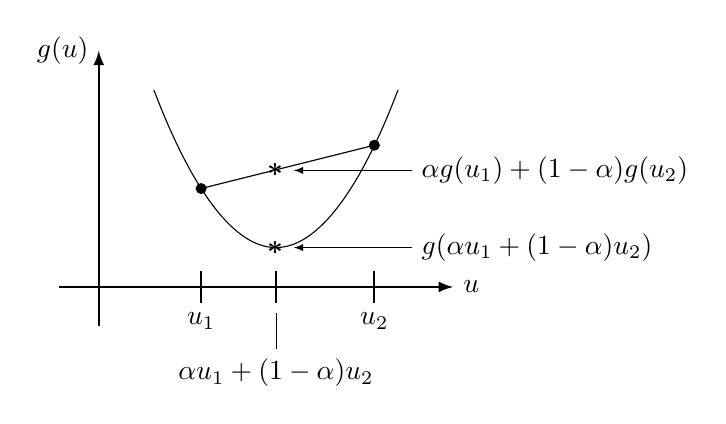
\begin{tikzpicture}
      \path [line,->] (-0.5,0) -- (4.5,0) node [anchor=west] {$u$};
      \path [line,->] (0,-0.5) -- (0,3) node [anchor=east] {$g(u)$};
      \draw (0.7,2.5) parabola bend (2.25,0.5) (3.8,2.5);
      \path [line] (1.3,-0.2) node [anchor=north] {$u_1$} -- (1.3,0.2);
      \path [line] (3.5,-0.2) node [anchor=north] {$u_2$} -- (3.5,0.2);
      \path [line] (2.25,-0.2) node [pin={[pin edge={black}] below:{$\alpha u_1 + (1-\alpha)u_2$}}] {} -- (2.25,0.2);
      \draw (1.3,1.25) -- (3.5,1.8);
      \fill (1.3,1.25) circle (0.07);
      \fill (3.5,1.8) circle (0.07);
      \node [pin={[pin edge={black,<-},pin distance=1.5cm] right:{$g(\alpha u_1 + (1-\alpha)u_2)$}}] at (2.25,0.5) {$\bm *$};
      \node [pin={[pin edge={black,<-},pin distance=1.5cm] right:{$\alpha g(u_1) + (1-\alpha)g(u_2)$}}] at (2.25,1.48) {$\bm *$};
    \end{tikzpicture}
  \end{center}
\end{defi}

\begin{thm}
  If $\pder{^2 g}{u^2} (u) \succeq 0$ $\forall u\in\mathbb R^m$, then $g$ is convex. ($\Longleftrightarrow$ for $g\in C^2$)
\end{thm}

\paragraph{Example} $\displaystyle \min_u u\trans Q u - b\trans u$ where $Q=Q\trans\succ 0$ (positive definite matrix)
\begin{align}
  \pder{g}{u} &= \pder{}{u} (u\trans Qu - b\trans u) \\
              &= u\trans Q\trans + u\trans Q - b\trans \\
              &= 2u\trans Q - b\trans \\[-3ex]
  \pder{^2 g}{u^2} &= 2Q
              & \pder{^2 g}{u^2} = \begin{bmatrix}
                \pder{^2 g}{u_1^2} & \cdots & \pder{^2 g}{u_1 \partial u_m} \\
                \vdots & \ddots & \vdots \\
                \pder{^2 g}{u_m \partial u_1} & \cdots & \pder{^2 g}{u_m^2}
              \end{bmatrix}
\end{align}
From $\pder{g}{u} = 2u\trans Q-b\trans = 0$,
\[ u = \frac12 Q^{-1} b \]
To see whether this is a minimizer, consider the Hessian. Since $Q \succ 0$, it follows that $\pder{^2 g}{u^2} (u^*) \succ 0$ and $u^*=\frac12 Q^{-1} b$ is a (local) minimizer. Additionally, since $\pder{^2 g}{u^2} \succ 0$, $g$ is convex and $u^*$ is a global minimizer. In fact, since we have strict convexity ($\succ 0$ rather than $\succeq 0$), it is the unique global minimizer.

In optimal control, \emph{local} is typically all we can ask for. In optimization, we can do better!

But wait, just because we know $\pder{g}{u}=0$, it doesn't follow that we can actually find $u^*$\dots

\section{Numerical Methods}
Idea: $u_{k+1}=u_k+\text{step}_k$. What should $\text{step}_k$ be? For small $\text{step}_k=\gamma_k v_k$,
\[ g(u_k \cdot \text{step}_k) = g(u_k) + \pder{g}{u}(u_k) \cdot \text{step}_k + o(\Vert \text{step}_k \Vert) = g(u_k) + \gamma_k \pder{g}{u}(u_k) v_k + o(\gamma_k) \]
A perfectly reasonable choice of step direction is
\[ v_k=-\pder{g\trans}{u}(u_k), \]
known as the \emph{steepest descend} direction. This produces
\[ g \Big( u_k - \gamma_k\pder{g}{u}(u_k) \Big) = g(u_k) - \gamma_k \left\Vert \pder{g}{u}(u_k) \right\Vert^2 + o(\gamma_k) \]

\begin{framed}
  \textbf{Steepest descent} \[ u_{k+1} = u_k - \gamma_k \pder{g\trans}{u} (u_k) \]
\end{framed}

\paragraph{Note:} \mbox{}
\begin{itemize}
\item What should $\gamma_k$ be?
\item This method ``pretends'' that $g(u)$ is linear. If we pretend $g(u)$ is quadratic, we get
  \[ u_{k+1} = u_k - \left( \pder{^2 g}{u^2} (u_k) \right)^{-1} \pder{g\trans}{u} (u_k), \]
  i.e.\ Newton's Method
\end{itemize}

\paragraph{This course:} steepest descent

\subparagraph{Step-size selection?} \mbox{}
\begin{itemize}
\item Choice 1: $\gamma_k=\gamma$ ``small'' $\forall k$; will get close to a minimizer if $u_0$ is close enough and $\gamma$ small enough

  Problems: \vspace{-1ex}
  \begin{itemize}
  \item You may not converge! (but you'll get close)
  \item You may go off to infinity (diverge)
  \end{itemize}

  \begin{center}
    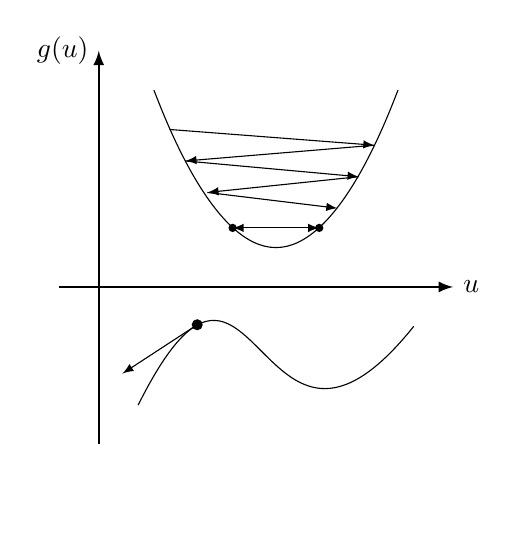
\begin{tikzpicture}
      \path [line,->] (-0.5,0) -- (4.5,0) node [anchor=west] {$u$};
      \path [line,->] (0,-2) -- (0,3) node [anchor=east] {$g(u)$};
      \draw (0.7,2.5) parabola bend (2.25,0.5) (3.8,2.5);
      \draw (0.5,-1.5) .. controls (2,1.5) and (2,-3) .. (4,-0.5);

      \draw [<->,>=latex] (1.7,0.75) node [circle,fill=black,minimum size=3pt,inner sep=0pt] {} -- (2.8,0.75) node [circle,fill=black,minimum size=3pt,inner sep=0pt] {};

      \draw [->,>=latex] (0.9,2) -- (3.5,1.8);
      \draw [->,>=latex] (3.5,1.8) -- (1.1,1.6);
      \draw [->,>=latex] (1.1,1.6) -- (3.3,1.4);
      \draw [->,>=latex] (3.3,1.4) -- (1.38,1.2);
      \draw [->,>=latex] (1.38,1.2) -- (3.03,1);

      \draw [->,>=latex] (1.25,-0.48) node [circle,fill=black,inner sep=0pt,minimum size=4pt] {} -- (0.3,-1.1);
    \end{tikzpicture}
  \end{center}
  
\item Choice 2: Reduce $\gamma_k$ as a function of $k$; will get close to a minimizer if $u_0$ is close enough

  Problem: slow

  \begin{thm}
    If $u_0$ is close enough to $u^*$ and $\gamma_k$ satisfies
    \begin{itemize}
    \item $\displaystyle \sum_{k=0}^\infty \gamma_k = \infty$
    \item $\displaystyle \sum_{k=0}^\infty \gamma_k^2 < \infty$
    \end{itemize}
    e.g.\ $\gamma_k=c/k$, then $u_k\to u^*$ as $k\to\infty$.
  \end{thm}
  
  % 2017/01/17
\item Choice 3: \textbf{Armijo step-size:} Take as big a step as possible, but no larger

  Pick $\alpha\in(0,1)$, $\beta\in(0,1)$. Let $i$ be the smallest non-negative integer such that
  \begin{gather}
    g\left( u_k - \beta^i \pder{g\trans}{u}(u_k) \right) - g(u_k) < -\alpha\beta^i \left\Vert \pder{g}{u}(u_k) \right\Vert^2 \\
    u_{k+1} = u_k - \beta^i \pder{g\trans}{u}(u_k)
  \end{gather}
  This will get to a minimizer blazingly fast if $u_0$ is close enough.
\end{itemize}

\section{Constrained Optimization}

Equality constraints:
\begin{align}
  \min_{u\in\mathcal R^m} {}\ & g(u) \\
  \text{s.t. } & h(u)=\bm 0
\end{align}
Consider $u\in\mathbb R^2$, $h:\mathbb R^2\to\mathbb R$
\begin{center}
  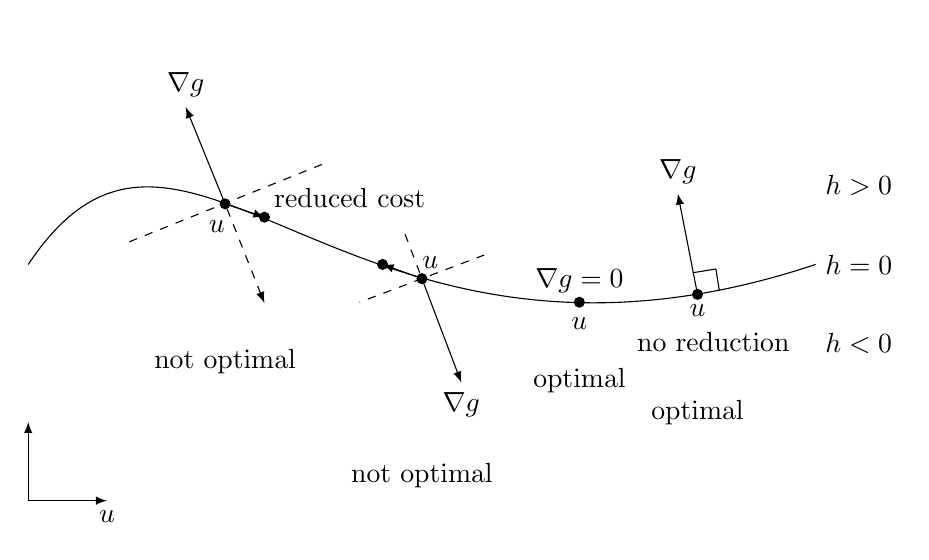
\begin{tikzpicture}[>=latex]
    \draw (0,0) .. controls (2,3) and (4,-2) .. (10,0) node [anchor=west] {$h=0$};
    \draw [>=latex,->] (0,-3) -- (0,-2);
    \draw [>=latex,->] (0,-3) -- (1,-3) node [anchor=north] {$u$};
    \node [anchor=west] at (10,1) {$h>0$};
    \node [anchor=west] at (10,-1) {$h<0$};

    \path
    coordinate (u) at (2.5,0.77)
    coordinate  (A) at (2,2)
    coordinate (B) at (3,-0.49)
    coordinate (C) at ($(u)!1!-90:(A)$)
    coordinate (D) at ($(A)!(C)!(B)$)
    coordinate (rc) at (3,0.6);
    \draw [->] (u) node [dot] {} -- (A) node [anchor=south] {$\nabla g$};
    \draw [<-,dashed] (B) -- (u) node [anchor=north,inner sep=6pt,xshift=-3pt] {$u$};
    \draw [dashed] (C) -- ($(C)!2!(D)$);
    \draw [->] (u) -- (rc) node [anchor=south west] {reduced cost};
    \node [circle,fill=black,inner sep=0pt,minimum size=4pt] at (rc) {};
    \node at ($(u)-(0,2)$) {not optimal};

    \draw [->]  (5,-0.18) node [dot] (u2) {} -- (5.5,-1.5) coordinate (A2);
    \node [anchor=north] at (A2) {$\nabla g$};
    \draw [dashed] (u2) node [anchor=south,xshift=3pt] {$u$} -- ($(A2)!1.5!(u2)$);
    \draw [dashed] ($(u2)!0.6!90:(A2)$) -- ($(u2)!0.6!-90:(A2)$);
    \draw [->] (u2) -- (4.5,-0) node [dot] {};
    \node at ($(u2)-(0,2.5)$) {not optimal};

    \node [dot] (u3) at (7,-0.48) {};
    \node [anchor=south] at (u3) {$\nabla g=0$};
    \node [anchor=north,yshift=-2pt] at (u3) {$u$};
    \node at ($(u3)-(0,1)$) {optimal};

    \draw [->] (8.5,-0.38) node [dot] (u4) {} -- (8.25,0.9) node [anchor=south] (A4) {$\nabla g$};
    \draw [shorten <=-0.5pt] ($(u4)!8pt!(A4)$) coordinate (B4) -- ($(B4)!1!90:(u4)$) coordinate (C4);
    \draw (C4) -- ($(C4)!1!90:(B4)$);
    \node [anchor=north] at (u4) {$u$};
    \node at ($(u4)-(-0.2,0.6)$) {no reduction};
    \node at ($(u4)-(0,1.5)$) {optimal};
  \end{tikzpicture}
\end{center}
So $u$ is (locally) optimal if $\nabla g \parallel$ (is parallel to) the normal vector to tangent plane to h.

\medskip
Fact: (HW\# 1)
\[ \nabla h \perp Th \quad \text{(tangent plane to h)} \]
\begin{center}
  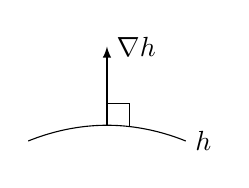
\begin{tikzpicture}
    \coordinate (u) at (1,0.2);
    \draw (0,0) parabola bend (u) (2,0) node [anchor=west] {$h$};
    \draw [->,>=latex] (u) -- ($(u)+(0,1)$) node [anchor=west] {$\nabla h$};
    \draw ($(u)+(0,8pt)$) coordinate (b) -- ($(b)!1!90:(u)$) coordinate (c);
    \draw [shorten >=-0.5pt] (c) -- ($(c)!1!90:(b)$);
  \end{tikzpicture}
\end{center}
We need $\nabla g \parallel \nabla h$ at $u^*$ for optimality, i.e.
\[ \pder{g}{u}(u^*) = \alpha \pder{h}{u}(u^*), \quad \text{for some } \alpha\in\R \]
or ($\lambda=-\alpha$),
\[ \pder{g}{u}(u^*) + \lambda \pder{h}{u}(u^*) = 0 \]
or
\[ \pder{}{u} \big( g(u^*) + \lambda h(u^*) \big) = 0, \quad \text{for some } \lambda\in\R \]
More generally,
\begin{align}
  \min_{u\in\mathcal R^m} {}\ & g(u) \\
  \text{s.t. } & h(u)=\bm 0, \quad h:\R^m\to\R^k
\end{align}
Note that $h(u)=[h_1(u),\dots,h_k(u)]\trans$.

We need $\pder{g}{u}(u^*)$ to be a linear combination of $\pder{h_i}{u}(u^*)$, $i=1,\dots,k$, for exactly the same reasons, i.e.
\[ \pder{g}{u}(u^*) = \sum_{i=1}^k \alpha_i \pder{h_i}{u}(u^*) \]
or ($\lambda=-[\alpha_1,\dots,\alpha_k]\trans$)
\[ \pder{g}{u}(u^*) + \lambda\trans \pder{h}{u}(u^*) = 0 \]
or
\[ \pder{}{u} \big( g(u^*) + \lambda\trans h(u^*) \big) = 0, \quad \text{for some } \lambda\in\R^k \]

\begin{thm}
  If $u^*$ is a minimizer to 
  \begin{align}
    \min_{u\in\mathcal R^m} {}\ & g(u) \\
    \text{s.t. } & h(u)=\bm 0, \quad h:\R^m\to\R^k
  \end{align}
  then $\exists\lambda\in\R^k$ s.t.
  \[ \begin{cases}
      \displaystyle \pder{L}{u}(u^*,\lambda) = 0 \\[2ex]
      \displaystyle \pder{L}{\lambda}(u^*,\lambda) = 0
    \end{cases} \]
  where the Lagrangian $L$ is given by
  \[ L(u,\lambda) = g(u) + \lambda\trans h(u) \]
\end{thm}

\paragraph{Note:}
\begin{itemize}
\item $\lambda$ are the Lagrange multipliers
\item $\pder{L}{\lambda}=0$ is fancy speak for $h(u^*)=0$
\end{itemize}

\paragraph{Example}
\begin{align}
  \min_{u\in\R^m} {}\ & \frac12 \Vert u\Vert^2 \\
  \text{s.t. } & Au=b
\end{align}
where $A$ is $k\times m$, $k\le m$. Assume $(AA\trans)^{-1}$ exists (constraints are linearly independent, none of the constraints are ``duplicates'', all the constraints are essential).
\begin{align}
  L &= \frac12 u\trans u + \lambda\trans (Au-b) \\
  \pder{L}{u} &= u\trans + \lambda\trans A = 0 \\
  u^* &= -A\trans \lambda \\
  \shortintertext{Using the equality constraint,}
  A u^* &= b \\
  -A A\trans \lambda &= b \\
  \lambda &= -(AA\trans)^{-1} b \\
  u^* &= A\trans (AA\trans)^{-1} b
\end{align}

\paragraph{Example}
\begin{align}
  \min {}\ & u_1u_2 + u_2u_3 + u_1u_3 \\
  \text{s.t. } & u_1 + u_2 + u_3 = 3
\end{align}
\[ L = u_1u_2 + u_2u_3 + u_1u_3 + \lambda (u_1 + u_2 + u_3 - 3) \]
\begin{align}
  \begin{cases}
    \pder{L}{u_1} = u_2 + u_3 + \lambda = 0 \\
    \pder{L}{u_2} = u_1 + u_3 + \lambda = 0 \\
    \pder{L}{u_3} = u_2 + u_1 + \lambda = 0 \\
    \pder{L}{\lambda} = u_1 + u_2 + u_3 = 3
  \end{cases}
  \Longrightarrow
  \begin{cases}
    u_1^* = 1 \\
    u_2^* = 1 \\
    u_3^* = 1 \\
    \lambda = -2
  \end{cases}
  \quad \text{optimal solution}
\end{align}
Note: This was actually the worst we can do---maximize! Even weirder: no local minimizer!

% 2017/01/19
\subsection{Equality Constraints}
\begin{align}
  \min_{u\in\mathcal R^m} {}\ & g(u) \\
  \text{s.t. } & h(u)=\bm 0, \quad h:\R^m\to\R^k
\end{align}
\begin{thm}
  If $u^*$ is a minimizer/maximizer then $\exists\lambda\in\R^k$ s.t.
  \begin{align}
    \pder{L}{u}(u^*,\lambda) &= 0 \\
    \pder{L}{\lambda}(u^*,\lambda) &= 0 \qquad (\Longleftrightarrow h(u^*)=0)
  \end{align}
  where $L(u,\lambda) = g(u) + \lambda\trans h(u)$.
\end{thm}

\paragraph{Example} [Entropy Maximization]

Given $S=\{x_1,\dots,x_n\}$ and a distribution over $S$ such that it takes the value $x_j$ with probability $p_j$. The entropy is
\[ E(p) = \sum_{j=1}^n (-p_j \ln p_j). \]
The mean is
\[ m = \sum_{j=1}^n p_jx_j. \]
Problem: Given $m$, find $p$ such that $E$ is maximized.
\begin{align}
  \min_{p} {}\ & -\sum_{j=1}^n p_j \ln p_j \\
  \text{s.t. } & \sum_{j=1}^n p_j x_j = m \\
               & \sum_{j=1}^n p_j = 1 \\
               & p_j \ge 0, \ j=1,\dots,n \quad \text{(ignore this\dots)}
\end{align}
\begin{align}
  L &= - \sum p_j \ln p_j + \lambda_1 \left[ \sum p_j x_j -m \right] + \lambda_2 \left[ \sum p_j - 1 \right] \\
  \pder{L}{p_j} &= -\ln p_j - 1 + \lambda_1 x_j + \lambda_2 = 0 \\
  p_j &= e^{\lambda_2 - 1 + \lambda_1 x_j}, \quad j=1,\dots,n \qquad (p_j\ge0 \text{ so we're ok with ignoring that})
\end{align}
\begin{align}
  \sum e^{\lambda_2 - 1 + \lambda_1 x_j} x_j &= m && n+2 \text{ equations and} \\
  \sum e^{\lambda_2 - 1 + \lambda_1 x_j} &= 1 && n+2 \text{ unknowns\dots}
\end{align}
No analytical solution, but numerically ``solvable''

\subsection{Inequality Constraints}
\begin{align}
  \min_{u\in\mathcal R^m} {}\ & g(u) \\
  \text{s.t. } & h(u)\le\bm 0, \quad h:\R^m\to\R^k
\end{align}
\begin{center}
  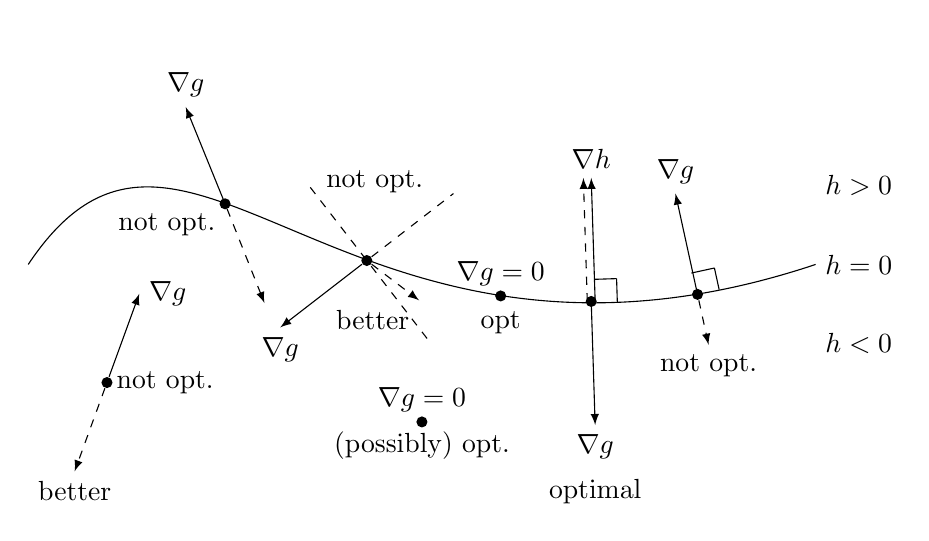
\begin{tikzpicture}[>=latex]
    \draw (0,0) .. controls (2,3) and (4,-2) .. (10,0) node [anchor=west] {$h=0$};
    \node [anchor=west] at (10,1) {$h>0$};
    \node [anchor=west] at (10,-1) {$h<0$};

    \path
    coordinate (u) at (2.5,0.77)
    coordinate  (A) at (2,2)
    coordinate (B) at (3,-0.49);
    \draw [->] (u) node [dot] {} -- (A) node [anchor=south] {$\nabla g$};
    \draw [<-,dashed] (B) -- (u) node [anchor=north east] {not opt.};

    \node [dot] (u3) at (6,-0.40) {};
    \node [anchor=south] at (u3) {$\nabla g=0$};
    \node [anchor=north,yshift=-2pt] at (u3) {opt};

    \coordinate (u2) at (7.2,-0.47);
    \coordinate (A2) at (7.15, 1.1);
    \draw [->] (u2) -- (A2) node [anchor=south] {$\nabla h$};
    \draw [->] ($(u2)+(-0.05,0)$) node [dot] {} -- ($(u2)!-1!(A2)+(-0.05,0)$) node [anchor=north] (D2) {$\nabla g$};
    \draw ($(u2)!8pt!(A2)$) coordinate (B2) -- ($(B2)!1!90:(u2)$) coordinate (C2);
    \draw [shorten >=-0.5pt] (C2) -- ($(C2)!1!90:(B2)$);
    \draw [->,dashed] ($(u2)+(-0.1,0)$) -- ($(A2)+(-0.1,0)$);
    \node [anchor=north,yshift=-8pt] at (D2) {optimal};

    \draw [->] (8.5,-0.38) node [dot] (u4) {} -- (8.22,0.9) coordinate (A4);
    \node [anchor=south] at (A4) {$\nabla g$};
    \draw [->,dashed] (u4) -- ($(u4)!-0.5!(A4)$) node [anchor=north] {not opt.};
    \draw [shorten <=-0.5pt] ($(u4)!8pt!(A4)$) coordinate (B4) -- ($(B4)!1!90:(u4)$) coordinate (C4);
    \draw (C4) -- ($(C4)!1!90:(B4)$);

    \node [dot] (u5) at (4.3,0.05) {};
    \draw [->] (u5) -- (3.2,-0.8) coordinate (a5);
    \node [anchor=north] at (a5) {$\nabla g$};
    \draw [dashed] (u5) -- ($(u5)!-1!(a5)$) coordinate (b5);
    \draw [dashed] ($(u5)!0.9!90:(a5)$) -- ($(u5)!0.9!90:(b5)$);
    \draw [->,dashed] (u5) -- ($(u5)!0.6!-75:(b5)$) node [anchor=north east] {better};
    \node at ($(u5)+(0.1,1)$) {not opt.};

    \node [dot] (u6) at (5,-2) {};
    \node [anchor=south] at (u6) {$\nabla g=0$};
    \node [anchor=north] at (u6) {(possibly) opt.};

    \node [dot] (u7) at (1,-1.5) {};
    \draw [->] (u7) -- +(70:1.2) coordinate (a7);
    \node [anchor=west] at (a7) {$\nabla g$};
    \draw [->,dashed] (u7) -- ($(u7)!-1!(a7)$) node [anchor=north] {better};
    \node [anchor=west] at (u7) {not opt.};
  \end{tikzpicture}
\end{center}

We need:
\begin{itemize}
\item if $h(u^*)<0$ then $\pder{g}{u}(u^*)=0$
\item if $h(u^*)=0$ then we need either
  \begin{gather}
    \pder{g}{u}(u^*) = 0 \\
    \shortintertext{or}
    \pder{g}{u}(u^*) = -\lambda\pder{h}{u}(u^*) \quad \text{for } \lambda>0
  \end{gather}
\end{itemize}
Or, even better,
\[ \pder{}{u} \left( g(u^*) + \lambda h(u^*) \right) = 0 \quad \text{for } \lambda\ge 0, \]
where $\lambda h(u^*)=0$. ($h<0\to\lambda=0$, $h=0\to\lambda\ge0$)

In general, if $u\in\R^m$ and $h:\R^m\to\R^k$, we have that $u^*$, if optimal, has to satisfy
\begin{gather}
  \pder{}{u} L(u^*,\lambda) = 0 \\
  h(u^*) \le \bm 0 \\
  \lambda\trans h(u^*) = 0 \\
  \lambda \ge \bm 0
\end{gather}
where the Lagrangian is $L(u,\lambda) = g(u) + \lambda\trans h(u)$. Note that if we're maximizing, the same holds except we need $\lambda\le 0$.

\paragraph{Example}
\begin{align}
  \min {}\ & 2u_1^2 + 2u_1u_2 + u_2^2 - 10u_1 - 10u_2 \\
  \text{s.t. } & \begin{cases}
    u_1^2 + u_2^2 \le 5 \\
    3u_1 + u_2 \le 6
  \end{cases}
\end{align}
\[ L = 2u_1^2 + 2u_1u_2 + u_2^2 - 10u_1 - 10u_2 + \lambda_1 (u_1^2 + u_2^2 - 5) + \lambda_2 (3u_1+u_2 - 6) \]
FONC:
\begin{enumerate}[label=\roman*)]
\item $\partial L/\partial u_1 = 4u_1 + 2u_2 - 10 + 2\lambda_1u_1 + 3\lambda_2$
\item $\partial L/\partial u_2 = 2u_1 + 2u_2 - 10 + 2\lambda_1u_2 + \lambda_2$
\item $u_1^2 + u_2^2 \le 5$
\item $3u_1 + u_2 \le 6$
\item $\lambda_1(u_1^2 + u_2^2 - 5) = 0$
\item $\lambda_2(3u_1 + u_2 - 6) = 0$
\item $\lambda_1 \ge 0$
\item $\lambda_2 \ge 0$
\end{enumerate}
To solve, assume different constraints are active/inactive:
\begin{enumerate}
\item Both constraints are inactive ($u_1^2 + u_2^2 < 5$, $3u_1 + u_2 < 6$) $\Longrightarrow \lambda_1=\lambda_2=0$
  \[ \begin{cases}
      4u_1 + 2u_2 - 10 = 0 \\
      2u_1 + 2u_2 - 10 = 0
    \end{cases}
    \Longrightarrow
    \begin{cases}
      u_1 = 0 \\
      u_2 = 5
    \end{cases} \]
  Note: iii) $0^2 + 5^2 \nleq 5$

  Not feasible

\item Assume constraint 1 is active and constraint 2 is inactive ($u_1^2 + u_2^2 = 5$, $\lambda_2=0$)
  \[ \begin{cases}
      4u_1 + 2u_2 - 10 + 2\lambda_1u_1 = 0 \\
      2u_1 + 2u_2 - 10 + 2\lambda_1u_2 = 0 \\
      u_1^2 + u_2^2 = 5
    \end{cases}
    \Longrightarrow
    \begin{cases}
      u_1 = 1 \\
      u_2 = 2 \\
      \lambda_1 = 1
    \end{cases} \]
  \begin{enumerate}[label=$\square$\hspace{1pt}\llap{\protect\raisebox{2pt}{$\checkmark$}}]
  \item $\lambda_1 \ge 0$
  \item $3\cdot 1 + 2 \le 6$
  \end{enumerate}
  This is a local minimizer

\item Assume constraint 2 is active and constraint 1 is inactive
\item Assume both constraints are active
\end{enumerate}

\paragraph{Kuhn-Tucker Conditions} (KKT conditions, Karush-Kuhn-Tucker)
\subparagraph{Problem:}
\begin{equation}
  \begin{aligned}
    \min_{u\in\R^m} {}\ & g(u) \\
    \text{s.t. } & \begin{cases}
      h_1(u) = 0, & h_1:\R^m\to\R^p \\
      h_2(u) \le 0, & h_2:\R^m\to\R^k
    \end{cases}
  \end{aligned}
  \label{eq:kkt}
\end{equation}

\begin{thm}
  Let $u^*$ be feasible ($h_1=0$, $h_2\le0$). If $u^*$ is a minimizer to \eqref{eq:kkt} than there exists vectors $\lambda\in\R^p$, $\mu\in\R^k$ with $\mu\ge\bm 0$ such that
  \[ \begin{cases}
      \displaystyle \pder{g}{u}(u^*) + \lambda\trans \pder{h_1}{u}(u^*) + \mu\trans \pder{h_2}{u}(u^*) = 0 \\[1ex]
      \mu\trans h_2(u^*) = 0
    \end{cases} \]
\end{thm}

Looking ahead: $\min \text{cost}(u(\cdot))$ s.t.\ $\dot x = f(x,u)$ (dynamics), where $u$ is a function. Note the equality constraint.

% 2017/01/24
\paragraph{Question:} How do we go from $u\in\R^m$ to $u\in\mathcal U$ (function space)?
\subparagraph{Note:} Function space is a set of functions of a given kind from a set $X$ to a set $Y$
\begin{enumerate}
\item linear function
\item square-integrable functions: $L_2[0,T]:$ $\int_0^T \Vert u(t)\Vert^2 \dif t < \infty$
\item $C^\infty (\R)$
\end{enumerate}
What would $\partial \text{``cost''}/\partial u$ mean?

\section{Directional Derivatives}
\paragraph{Recall:} To minimize $g(u)$, let $u^*$ be a candidate minimizer and pitch a perturbation on $u^*$ of $\varepsilon v$, where $\varepsilon$ is the scale and $v$ is the direction. Taking Taylor's expansion at the perturbation produces

\begin{center}
  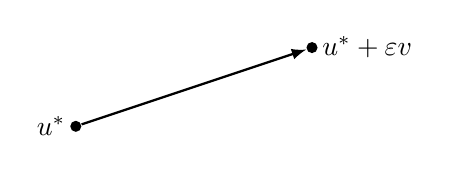
\begin{tikzpicture}
    \node [dot] (a) at (0,0) {};
    \node [dot] (b) at (3,1) {};
    \draw [>=latex,->,thick] (a) node [anchor=east] {$u^*$} -- (b) node [anchor=west] {$u^*+\varepsilon v$};
  \end{tikzpicture}
\end{center}

\begin{gather}
  g(u^* + \varepsilon v) = g(u^*) + \varepsilon \pder{g}{u}(u^*) v + o(\varepsilon) \\
  \text{FONC: } \pder{g}{u}(u^*) = 0 \hspace{3cm} 
\end{gather}

\subparagraph{Note:} $\pder{g}{u}(u^*) v$ tells us how much $g(u)$ increases/decreases in the direction of $v$.

\begin{defi}
  The directional (Gateaux) derivative is given by
  \[ \delta g(u;v) = \lim_{\varepsilon\to0} \frac{g(u+\varepsilon v)-g(u)}{\varepsilon} \]
\end{defi}

\paragraph{Example}
\[ g(u) = \frac12 u_1^2 - u_1 + 2u_2, \quad g:\R^2\to\R \]
Let's consider $e_1=[1\ 0]\trans$, $e_2=[0\ 1]\trans$. What is $\delta g(u;e_i)$, $i=1,2$?
\begin{align}
  \delta g(u;v) &= \lim_{\varepsilon\to0} \frac{g(u+\varepsilon v)-g(u)}{\varepsilon} \\
                &= \lim_{\varepsilon\to0} \frac{g(u)+\varepsilon\pder{g}{u}(u) v + o(\varepsilon) - g(u)}{\varepsilon} \\
                &= \pder{g}{u} (u) v
\end{align}
\begin{align}
  \pder{g}{u}(u) &= [u_1-1\ 2] \\
  \delta g(u;e_1) &= [u_1-1\ 2] e_1 = u_1-1 \\
  \delta g(u;e_2) &= [u_1-1\ 2] e_2 = 2 \\
\end{align}

But the beauty of directional derivatives is that they generalize beyond vectors, $u\in\R^m$, to function spaces ($\mathcal U$) or other ``objects'' like matrices.

\paragraph{Example} $M\in\R^{n\times n}$, $F(M)=M^2$

What is $\pder{F}{M}$? (ponder at home\dots)

We can easily compute $\delta F(M;N)$!
\begin{align}
  F(M+\varepsilon N) &= (M+\varepsilon N)(M+\varepsilon N) = M^2 + \varepsilon M N + \varepsilon N M + \varepsilon^2 N^2 \\
  \delta F(M;N) &= \lim_{\varepsilon\to0} \frac{F(M+\varepsilon N)-F(M)}{\varepsilon} \\
                     &= \lim_{\varepsilon\to0} \frac{\varepsilon M N + \varepsilon N M + \varepsilon^2 N^2}{\varepsilon} = MN + NM
\end{align}

\paragraph{Infinite Dimensional Optimization}
Let $u\in\mathcal U$ (function space) and let $J(u)$ be the cost:
\[ \min_{u\in\mathcal U} J(u) \]

\begin{thm}
  If $u^*\in\mathcal U$ is a (local) minimizer then
  \[ \delta J(u^*;v) = 0, \quad \forall v\in\mathcal U \]
\end{thm}

\paragraph{Example} Find minimizer $u^*$ to
\[ J(u) = \int_0^T L(u(t)) \dif t \]
\begin{align}
  J(u+\varepsilon v) - J(u) &= \int_0^T L(u(t)+\varepsilon v(t)) \dif t - \int_0^T L(u(t)) \dif t, \quad u,v\in\mathcal U \\
                            &= \int_0^T \left[ L(u(t)) + \varepsilon \pder{L}{u}(u(t)) v(t) + o(\varepsilon) - L(u(t)) \right] \dif t \\
  \delta J(u^*;v) &= \lim_{\varepsilon\to0} \frac{J(u+\varepsilon v)-J(u)}{\varepsilon} \\
                            &= \lim_{\varepsilon\to0} \frac{\int_0^T \varepsilon \pder{L}{u}(u(t)) v(t) \dif t + o(\varepsilon)}{\varepsilon} \\
                            &= \int_0^T \pder{L}{u}(u(t)) v(t) \dif t \\
\end{align}
$u^*$ optimizer:
\begin{gather}
  \delta J(u^*;v) = \int_0^T \pder{L}{u}(u(t)) v(t) \dif t = 0 \quad \forall v\in\mathcal U \\
  \Updownarrow \\
  \pder{L}{u} (u(t)) = 0 \quad \forall t\in[0,T]
\end{gather}
But, we want \emph{optimal control}! We want our cost to look like
\begin{gather}
  \int_0^T L(x(t),u(t)) \dif t \\
  \dot x = f(x,u)
\end{gather}

\section{Calculus of Variations}
What happens to $x(t)$ when $u(t)$ changes to $u(t)+\varepsilon v(t)$? Let the system be given by
\[ \begin{cases}
    \dot x = f(x,u) \\
    x(0) = x_0
  \end{cases} \]
After perturbation of $u$, the new system is
\[ \begin{cases}
    \dot{\hat x} = f(\hat x,u+\varepsilon v) \\
    x(0) = x_0
  \end{cases} \]

\pgfmathsetseed{11}
\begin{figure}
  \centering
  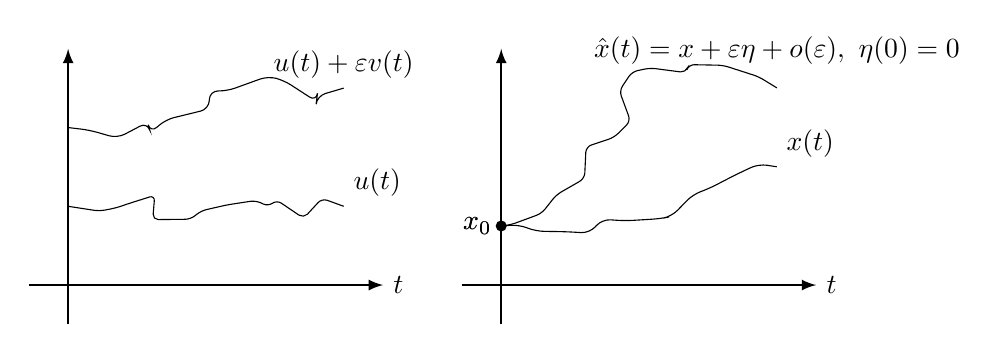
\begin{tikzpicture}
    \draw [thick,->] (-0.5,0) -- (4,0) node [anchor=west] {$t$};
    \draw [thick,->] (0,-0.5) -- (0,3) node [anchor=east] {};
    \draw [decorate, decoration={random steps, segment length=7pt, amplitude=5pt}, rounded corners=2pt] (0,1) to[in=180,out=0,distance=3.5cm] (3.5,1) node [anchor=south west] {$u(t)$};
    \draw [decorate, decoration={random steps, segment length=8pt, amplitude=5pt}, rounded corners=3pt] (0,2) to[in=180,out=0,distance=3cm] (3.5,2.5) node [anchor=south] {$u(t)+\varepsilon v(t)$};

    \draw [thick,->] (5,0) -- (9.5,0) node [anchor=west] {$t$};
    \draw [thick,->] (5.5,-0.5) -- (5.5,3) node [anchor=east] {};
    \draw [decorate, decoration={random steps, segment length=8pt, amplitude=4pt}, rounded corners=3pt] (5.5,0.75) node [anchor=east] {$x_0$} to[in=200,out=0,distance=3cm] (9,1.5) node [anchor=south west] {$x(t)$};
    \draw [decorate, decoration={random steps, segment length=8pt, amplitude=5pt}, rounded corners=2pt] (5.5,0.75) node [anchor=east] {$x_0$} to[in=170,out=30,distance=3cm] (9,2.5) node [anchor=south,yshift=5pt] {$\hat x(t)=x+\varepsilon\eta+o(\varepsilon),\ \eta(0)=0$};
    \node [dot] at (5.5,0.75) {};
  \end{tikzpicture}
  \caption{Variation in $u$ causes a variation in $x$.}
  \label{fig:var_u_x}
\end{figure}

\noindent
Consider
\[ \tilde x=x+\varepsilon \eta, \]
where
\begin{alignat}{2}
  \dot x&=f(x,u), & x(0) &= x_0 \\
  \dot \eta &= \pder{f}{x}(x,u) \eta + \pder{f}{u}(x,u) v, \qquad & \eta(0) &= 0
\end{alignat}

\begin{thm}
  If $f$ is continuously differentiable in $x$ and $u$ then
  \[ \hat x(t) = \tilde x(t) + o(\varepsilon) \]
  \begin{proof}
    \mbox{}
    \begin{enumerate}[label=\roman*)]
    \item Initial conditions:
      \begin{align}
        \hat x(0) &= x_0 \\
        \tilde x(0) &= x(0) + \varepsilon \eta(0) = x_0
      \end{align}
    \item Dynamics:
      \begin{align}
        \dot{\hat x} &= f(\hat x,u+\varepsilon v) \\
        \dot{\tilde x} &= \dot x + \varepsilon \dot \eta = f(x,u) + \varepsilon \pder{f}{x}(x,u)\eta + \varepsilon \pder{f}{u}(x,u) v \\
                     &= f(x+\varepsilon\eta,u+\varepsilon v) + o(\varepsilon) \\
                     &= f(\tilde x,u+\varepsilon v) + o(\varepsilon)
      \end{align}
      We can see that the dynamics of $\hat x(t)$ are equal to those of $\tilde x(t)$ plus higher order terms:
      \begin{align}
        \dot{\tilde x} &= f(\tilde x,u+\varepsilon v) + o(\varepsilon) \\
        \dot{\hat x} &= f(\hat x,u+\varepsilon v)
      \end{align}
      Therefore, if our perturbation is small enough, we can model $\hat x(t)$ as $\tilde x(t)$.
    \end{enumerate}
  \end{proof}
\end{thm}

\begin{framed}
  \hypertarget{taylor_2var}{}
  Note: Taylor expansion with two elements is
  \begin{align}
    h(w+\varepsilon v,z+\varepsilon y) &= h(w,z+\varepsilon y) + \pder{h}{w}(w,z+\varepsilon y)\varepsilon v + o(\varepsilon) \\
                                       &= \left\{ h(w,z) + \pder{h}{z}(w,z)\varepsilon y + o(\varepsilon) \right\} \\
                                       & \qquad + \left\{ \pder{h}{w}(w,z)\varepsilon v + \underbrace{\pder{^2 h}{z\partial w}\varepsilon v \odot \varepsilon y}_{o(\varepsilon)} + o(\varepsilon) \right\} \\
                                       &= h(w,z) + \pder{h}{z}\varepsilon y + \pder{h}{w}\varepsilon v + o(\varepsilon)
  \end{align}
\end{framed}

% 2017/01/26
\paragraph{Last class:} \mbox{}
\begin{enumerate}
\item $u\in\U$ (space of functions), $J:\U\to\R$ (cost).

  FONC: If $u^*$ is optimal, then
  \[ \delta J(u;\nu) = 0 \quad \forall \nu\in\U, \]
  where the directional derivative is given by
  \[ \delta J(u;\nu) = \lim_{\varepsilon\to0} \frac{J(u+\varepsilon \nu)-J(u)}{\varepsilon}. \]
\item If
  \[ \begin{cases}
      \dot x = f(x,u) \\
      x(0) = x_0
    \end{cases} \]
  then a variation in $u$:
  \[ u \longmapsto u+\varepsilon \nu \]
  results in a variation in $x$:
  \[ x \longmapsto x+\varepsilon\eta + o(\varepsilon) \]
  See \autoref{fig:var_u_x}. Note $\eta(0)=0$.
\end{enumerate}

\subsection{An (Almost) Optimal Control Problem}

Let $\dot x=f(x)$, $x(0)=x_0$. Note we get to pick the initial condition!
\subparagraph{Problem}
\begin{gather}
  \min_{x_0\in\R^m} J(x_0) = \int_0^T L(x(t)) \dif t \\
  \text{s.t. } \begin{cases}
    \dot x(t) = f(x(t)) & \text{the \emph{constraint}! (equality)} \\
    x(0)=x_0
  \end{cases}
\end{gather}
Note every constraint needs a Lagrange multiplier. We have infinitely many constraints:
\[ \dot x(t) = f(x(t)) \quad \forall t\in[0,T] \]
We need $\lambda(t)$ as a function of $t$. Also, the sum in the Lagrangian has to become an integral. The continuous-time Lagrangian thus becomes
\[ \tilde J(x_0,\lambda) = \int_0^T \Big[ L(x(t)) + \lambda\trans(t) (f(x(t))-\dot x(t)) \Big] \dif t \]
The task is to perturb $x_0$ as $x_0\longmapsto x_0+\varepsilon \nu$, $\nu\in\R^m$ and compute
\[ \delta \tilde J(x_0;\nu) = \lim_{\varepsilon\to0} \frac{\tilde J(x_0+\varepsilon \nu)-\tilde J(x_0)}{\varepsilon} \]
and make this equal to 0 $\forall \nu\in\R^m$. The variation in $x$ is

\pgfmathsetseed{11}
\begin{center}
  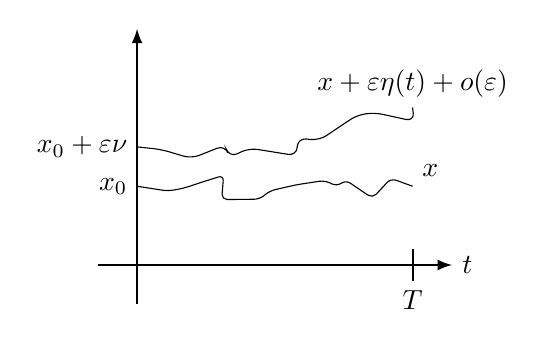
\begin{tikzpicture}
    \draw [->,thick] (-0.5,0) -- (4,0) node [anchor=west] {$t$};
    \draw [->,thick] (0,-0.5) -- (0,3);
    \draw [decorate, decoration={random steps, segment length=7pt, amplitude=5pt}, rounded corners=2pt] (0,1) node [anchor=east] {$x_0$} to[in=180,out=0,distance=3.5cm] (3.5,1) node [anchor=south west] {$x$};
    \draw [decorate, decoration={random steps, segment length=9pt, amplitude=5pt}, rounded corners=3pt] (0,1.5) node [anchor=east] {$x_0+\varepsilon \nu$} to[in=200,out=0,distance=3.5cm] (3.5,2) node [anchor=south] {$x+\varepsilon\eta(t)+o(\varepsilon)$};
    \draw [thick] (3.5,0.2) -- (3.5,-0.2) node [anchor=north] {$T$};
  \end{tikzpicture}
\end{center}

Note:

\hspace{\parindent}
\begin{tabular}{cl}
  $x_0$ & decision variable \\
  $\nu$ & variation in $x_0$ \\
  $x(t)$ & trajectory starting at $x_0$ \\
  $\eta(t)$ & change in trajectory resulting from $\nu$-variation in $x_0$ \\
  $\lambda(t)$ & time-varying Lagrange multiplier
\end{tabular}

\begin{align}
  \tilde J(x_0+\varepsilon \nu) &= \int_0^T \Big\{ L(x(t)) + \lambda\trans(t) [f(x(t)+\varepsilon\eta(t)) - \dot x(t) - \varepsilon\dot\eta(t)] \Big\} \dif t + o(\varepsilon) \\
                                &= \int_0^T \left[ L(x) + \varepsilon\pder{L}{x}(x)\eta + \lambda\trans \left( f(x) + \varepsilon\pder{f}{x}(x)\eta - \dot x - \varepsilon\dot\eta \right) \right] \dif t + o(\varepsilon) \\
  \tilde J(x_0+\varepsilon \nu) - \tilde J(x_0) &= \int_0^T \left[ \varepsilon\pder{L}{x}(x)\eta + \lambda\trans\left( \varepsilon\pder{f}{x}\eta - \varepsilon\dot\eta \right) \right] \dif t + o(\varepsilon) \\
  \delta \tilde J (x_0;\nu) &= \int_0^T \left[ \pder{L}{x}(x)\eta + \lambda\trans\left( \pder{f}{x}\eta - \dot\eta \right) \right] \dif t
\end{align}
A powerful idea: we want $\delta\tilde J(x_0;\nu)=0$ $\forall \nu$. Somehow get this in the form
\[ \int_0^T \Big(\text{stuff}(t)\Big) \eta(t) \dif t = 0 \]
We can pick $\text{stuff}(t)=0$ $\forall t\in[0,T]$.

In $\delta\tilde J(x_0;\nu)$ we have $\dot\eta$ (problem!). We can solve this using \emph{integration by parts}.
\[ \int_0^T \lambda\trans \dot\eta \dif t = \lambda\trans(T)\eta(T) - \lambda\trans(0)\eta(0) - \int_0^T \dot\lambda\trans\eta \dif t \]
Hence,
\[
  \delta\tilde J(x_0;\nu) = \int_0^T \underbrace{\big( \pder{L}{x} + \lambda\trans\pder{f}{x} + \dot\lambda\trans \big)}_{\text{pick}=0} \eta \dif t - \underbrace{\lambda\trans(T)}_{\text{pick}=0} \eta(T) + \lambda\trans(0) \underbrace{\eta(0)}_{\nu}
\]
We are free to pick $\lambda$ freely if it gives $\delta\tilde J=0$.
\[ \text{Pick: } \begin{cases}
    \dot\lambda(t) = -\pder{L\trans}{x}(x(t)) - \pder{f\trans}{x}(x(t)) \lambda(t) \\
    \lambda(T) = 0 & \text{backwards diff. eq}
  \end{cases} \]
Under this choice of $\lambda$ we get
\[ \delta\tilde J(x_0;\nu) = \lambda\trans(0) \nu \]
This is linear in $\nu$ so the FONC is $\lambda(0)=0$.

Moreover, we really have a ``normal'' optimization problem
\begin{gather}
  \min_{x_0\in\R^m} \tilde J(x_0) \\
  \delta \tilde J(x_0;\nu) = \pder{\tilde J}{x_0} (x_0) \nu
\end{gather}
which means that
\[ \pder{\tilde J}{x_0} = \lambda\trans(0) \]
If $x_0^*$ minimizes
\begin{gather}
  \int_0^T L(x(t)) \dif t \\
  \text{s.t. } \begin{cases}
    \dot x(t) = f(x(t)) \\
    x(0) = x_0^*
  \end{cases}
\end{gather}
then
\[ \lambda(0) = \bm 0 \]
where $\lambda(t)$ satisfies
\[ \begin{cases}
    \dot \lambda(t) = -\pder{L\trans}{x}(x(t)) - \pder{f\trans}{x}(x(t)) \lambda(t) \\
    \lambda(T) = 0
  \end{cases} \]

\paragraph{So what?} We actually have a two-point boundary value problem. 
\begin{align}
  \dot x &= f(x) & \dot\lambda &= -\pder{L\trans}{x} - \pder{f\trans}{x} \lambda \\
  x(0) &= x_0 & \lambda(T) &= 0
\end{align}

\begin{center}
  \begin{tikzpicture}
    \draw [thick,->] (0,0) -- (4,0) node [anchor=west] {$t$};
    \draw [thick,->] (0,0) -- (0,3);
    \draw (-0.2,1.5) node [anchor=east] {$x_0$} -- (0.2,1.5);
    \draw [->,>={Straight Barb[scale length=2]}] (0,1.5) parabola bend (0.6,2) (1.5,1.5);
    \draw (1.5,1.5) parabola bend (2,1.3) (3.5,2.5);

    \draw [thick,->] (6,0) -- (10,0) node [anchor=west] {$t$};
    \draw [thick,->] (6,0) -- (6,3);
    \draw (9.5,0.2) -- (9.5,-0.2) node [anchor=north] {$T$};
    \draw [-{Straight Barb[scale length=2]}] (9.5,0) .. controls (8.25,0) and (9,1.5) .. (8,1.5) node [anchor=south] {$\lambda$};
    \draw (8,1.5) .. controls (7,1.25) .. (6,1.5);
    \draw (6.2,1.5) -- (5.8,1.5) node [anchor=east] {$\lambda(0)$};
  \end{tikzpicture}
\end{center}
We want to find $x_0$ that gives $f(x)$ such that after solving backwards for $\lambda(t)$, we find that
\[ \lambda(0) = \pder{\tilde J\trans}{x_0} = 0. \]
This leads to the following:

\paragraph{An algorithm} \mbox{}

\begin{algorithm}
  \begin{algorithmic}
    \State Pick $x_{0,0}$
    \State $k=1$
    \Repeat
    \State Simulate $x(t)$ from $x_{0,k}$ over $[0,T]$
    \State Simulate $\lambda(t)$ from $\lambda(T)=0$ backwards using $x(t)$
    \State Update $x_{0,k}$ as
    $ x_{0,k+1} = x_{0,k} - \gamma\lambda(0) $ \Comment{$\lambda(0)$ is the gradient}
    \State $k\coloneqq k+1$
    \Until $\lambda(0)=0$
  \end{algorithmic}
\end{algorithm}

\paragraph{Example:} \texttt{optinit.m}

\[ \dot x = Ax, \quad L=x\trans Qx-q, \quad Q=Q\trans \succ 0 \]
\vspace{-2em}
\begin{align}
  \dot \lambda &= -2Qx - A\trans\lambda \\
  \lambda(0) &= 0
\end{align}

% 2017/01/31
\subsection{Optimal Timing Control}
When to switch between modes?
\begin{equation}
  \begin{aligned}
    \dot x &= \begin{cases}
      f_1(x) & \text{if } t\in[0,\tau) \\
      f_2(x) & \text{if } t\in[\tau,T]
    \end{cases} \\
    x(0) &= x_0
  \end{aligned} \label{eq:otc}
\end{equation}

\begin{center}
  \begin{tikzpicture}
    \draw [->,thick] (-0.2,0) -- (5.5,0) node [anchor=west] {$t$};
    \draw [->,thick] (0,-0.2) -- (0,3.2);
    \draw (4.8,0.2) -- (4.8,-0.2) node [anchor=north] {$T$};
    \draw (2.2,0.2) -- (2.2,-0.2) node [anchor=north] {$\tau$};
    \draw (0.2,1) -- (-0.2,1) node [anchor=east] {$x_0$};
    \draw (0,1) parabola (2.2,2.8);
    \draw (2.2,2.8) parabola [bend at end] (4.8,1.2) node [anchor=west] {$x$};
    \node at (1,1.8) {$f_1$};
    \node at (4,1.8) {$f_2$};
  \end{tikzpicture}
\end{center}

\begin{align}
  & \min_\tau \int_0^T L(x(t)) \dif t = J(\tau) \\
  & \text{s.t.~\eqref{eq:otc} holds}
\end{align}

\begin{enumerate}[label=Step \arabic*:]
\item Augment cost with constraint
  \[ \tilde J = \int_0^\tau \Big[ L(x) + \lambda\trans(f_1(x)-\dot x) \Big] \dif t + \int_\tau^T \Big[ L(x) + \lambda\trans(f_2(x)-\dot x) \Big] \dif t \]
\item Variation $\tau\longmapsto\tau+\varepsilon\theta$
  \begin{center}
    \begin{tikzpicture}
      \draw [->,thick] (-0.2,0) -- (5.5,0) node [anchor=west] {$t$};
      \draw [->,thick] (0,-0.2) -- (0,3.2);
      \draw (4.8,0.2) -- (4.8,-0.2) node [anchor=north] {$T$};
      \draw (2.2,0.2) -- (2.2,-0.2) node [anchor=north] {$\tau$};
      \draw (3,0.2) -- (3,-0.2) node [anchor=north,yshift=3pt] {$\tau+\varepsilon\theta$};
      \draw (0.2,1) -- (-0.2,1) node [anchor=east] {$x_0$};
      \draw (0,1) parabola (2.2,1.8);
      \draw (2.2,1.8) parabola [bend at end] (4.8,1.2) node [anchor=west] {$x$};
      \node at (1,1.8) {$f_1$};
      \node at (3.6,1.7) {$f_2$};

      \begin{scope}
        \clip (4.8,4) rectangle (2.2,1.8);
        \draw [dashed] (2.2,1.8) parabola bend (0,1) (3,2.5);
        \draw [dashed] (3,2.5) parabola [bend at end] (5.4,1.9);
      \end{scope}
      \node [anchor=west] at (4.8,1.9) {$x+\varepsilon\eta+o(\varepsilon)$};
      \node at (2.4,2.4) {$f_1$};
      \node at (3.9,2.5) {$f_2$};
    \end{tikzpicture}
  \end{center}
\item Compute $\delta\tilde J(\tau;\theta)$
\end{enumerate}
\begin{align}
  \tilde J(\tau+\varepsilon\theta) &= \int_0^{\tau+\varepsilon\theta} \Big\{ L(x+\varepsilon\eta) + \lambda\trans[f_1(x+\varepsilon\eta)-\dot x-\varepsilon\dot\eta] \Big\} \dif t \\
                                   & \qquad + \int_{\tau+\varepsilon\theta}^T \Big\{ L(x+\varepsilon\eta) + \lambda\trans[f_2(x+\varepsilon\eta)-\dot x-\varepsilon\dot\eta] \Big\} \dif t + o(\varepsilon) \\
  \intertext{Note that $\eta=\dot\eta=0$ on $[0,\tau)$.}
  \tilde J(\tau+\varepsilon\theta) &= \int_0^\tau \Big\{ L(x) + \lambda\trans[f_1(x)-\dot x] \Big\} \dif t \\
                                   & \qquad + \int_\tau^{\tau+\varepsilon\theta} \Big\{ \underbrace{L(x+\varepsilon\eta)}_{L(x)+\varepsilon\pder{L}{x}\eta} + \lambda\trans[\underbrace{f_1(x+\varepsilon\eta)}_{f_1(x)+\varepsilon\pder{f_1}{x}\eta} - \dot x-\varepsilon\dot\eta] \Big\} \dif t \\
                                   & \qquad + \int_{\tau+\varepsilon\theta}^T \Big\{ \underbrace{L(x+\varepsilon\eta)}_{L(x)+\varepsilon\pder{L}{x}\eta} + \lambda\trans[\underbrace{f_2(x+\varepsilon\eta)}_{f_2(x)+\varepsilon\pder{f_2}{x}\eta} - \dot x-\varepsilon\dot\eta] \Big\} \dif t + o(\varepsilon) \displaybreak \\
  \delta\tilde J(\tau;\theta) &= \lim_{\varepsilon\to0} \frac{\tilde J(\tau+\varepsilon\theta) - \tilde J(\tau)}{\varepsilon} \\
  \tilde J(\tau+\varepsilon\theta) - \tilde J(\tau) &= \int_0^\tau 0\cdot\dif t + \underbrace{ \int_\tau^{\tau+\varepsilon\theta} \left[ \varepsilon\pder{L}{x}\eta + \lambda\trans \Big(f_1(x)+\varepsilon\pder{f_1}{x}\eta - f_2(x) - \varepsilon\dot\eta \Big) \right] \dif t }_{\displaystyle I_1} \\
                                   & \qquad + \underbrace{ \int_{\tau+\varepsilon\theta}^T \left[ \varepsilon\pder{L}{x}\eta + \lambda\trans \Big( \varepsilon\pder{f_2}{x}\eta - \varepsilon\dot\eta \Big) \right] \dif t }_{\displaystyle I_2} + o(\varepsilon)
\end{align}

\begin{framed}
  \begin{thm}[Mean-value theorem]
    \[ \int_{t_1}^{t_2} h(t) \dif t = (t_2-t_1) h(\xi) \quad \text{for some}\ \xi\in[t_1,t_2] \]
  \end{thm}
\end{framed}

\noindent
The first integral is
\begin{align}
  I_1 &= \int_\tau^{\tau+\varepsilon\theta} \left\{ \varepsilon\pder{L}{x}\eta + \lambda\trans \left[f_1(x)+\varepsilon\pder{f_1}{x}\eta-\varepsilon\dot\eta-f_2(x)\right] \right\} \dif t \\
      &= \varepsilon\theta \Big\{ \lambda\trans(\xi) \big[ f_1(x(\xi)) - f_2(x(\xi)) \big] \Big\} + o(\varepsilon)
\end{align}
Note that as $\varepsilon\to0$, $\xi\to\tau$. Using integration by parts, the second integral is
\begin{align}
  \int_\tau^T \lambda\trans \dot\eta \dif t &= \lambda\trans(T) \eta(T) - \lambda\trans(\tau) \underbrace{\eta(\tau)}_{=0} - \int_\tau^T \dot\lambda\trans \eta \dif t \\
  I_2 &= \int_\tau^T \left[ \varepsilon\pder{L}{x}\eta + \lambda\trans \Big( \varepsilon\pder{f_2}{x}\eta - \varepsilon\dot\eta \Big) \right] \dif t - \underbrace{ \int_\tau^{\tau+\varepsilon\theta} \left[ \varepsilon\pder{L}{x}\eta + \lambda\trans \Big( \varepsilon\pder{f_2}{x}\eta - \varepsilon\dot\eta \Big) \right] \dif t }_{o(\varepsilon)} \\
                                            &= \varepsilon \int_\tau^T \left[ \pder{L}{x} + \lambda\trans \pder{f_2}{x} + \dot\lambda\trans \right] \eta \dif t - \varepsilon \lambda\trans(T)\eta(T) + o(\varepsilon)
\end{align}
Hence,
\begin{align}
  \delta\tilde J(\tau;\theta) &= \lim_{\varepsilon\to0} \frac{\tilde J(\tau+\varepsilon\theta) - \tilde J(\tau)}{\varepsilon} \\
                              &= \theta\lambda\trans(\tau) \Big[ f_1(x(\tau)) - f_2(x(\tau)) \Big] + \int_\tau^T \left[ \pder{L}{x} + \lambda\trans \pder{f_2}{x} + \dot\lambda\trans \right] \eta \dif t - \lambda\trans(T)\eta(T)
\end{align}

\begin{enumerate}[resume*]
\item Select the \emph{costate} $\lambda(t)$. The key idea is to get rid of any term that has $\eta$ in it, i.e.
  \begin{align}
    \dot\lambda &= -\pder{L\trans}{x} - \pder{f_2\trans}{x} \lambda \quad \text{on } [\tau,T] \\
    \lambda(T) &= 0
  \end{align}
\item With this choice of $\lambda(t)$, we have
  \[ \delta\tilde J(\tau;\theta) = \theta\lambda\trans(\tau) \Big[ f_1(x(\tau)) - f_2(x(\tau)) \Big] = \pder{\tilde J}{\tau} \theta. \]
  Therefore,
  \[ \pder{\tilde J}{\tau} = \lambda\trans(\tau) \Big[ f_1(x(\tau)) - f_2(x(\tau)) \Big] = 0 \quad \text{(for optimality)} \]
\end{enumerate}

\paragraph{Algorithm} \mbox{}
\begin{algorithm}
  \begin{algorithmic}
    \State Pick $\tau_0$
    \State $k=0$
    \Repeat
    \State Simulate $x$ forward in time from $x(0)=x_0$
    \State Simulate $\lambda$ backwards from $\lambda(T)=0$
    \State Update $\tau_k$ as
    $ \tau_{k+1} = \tau_k - \gamma\lambda\trans(\tau_k) \big[ f_1(x(\tau_k)) - f_2(x(\tau_k)) \big] $
    \State $k\coloneqq k+1$
    \Until $\Vert \lambda\trans(f_1-f_2) \Vert < \varepsilon$
  \end{algorithmic}
\end{algorithm}

Where are we going? Come up with general principles for $\min_{u\in\mathcal U} J(u)$:
\begin{itemize}
\item Costate equations
\item Optimality conditions
\item Algorithms
\item Applications
\end{itemize}

% 2017/02/02
\subsection{The Bolza Problem}
Up until now, we have optimized with respect to finite-dimensional parameters. Today, we will minimize with respect to $u\in\mathcal U$.

\begin{align}
  & \min_{u\in\mathcal U} J(u) = \int_0^T L(x(t),u(t),t) \dif t + \underbrace{\Psi(x(T))}_{\substack{\text{terminal cost}\\ \text{(parking cost)}}} \\
  & \begin{aligned}
    \text{s.t.}\quad \dot x(t) &= f(x(t),u(t),t) \\
    x(0) &= x_0
  \end{aligned}
\end{align}
Assume that $f$ and $L$ are $C^1$ in $x,u$ and piecewise continuous in $t$. Then, a small change in $u$ causes small changes in $f$ and $L$. The variation: $u\longmapsto u+\varepsilon v$, $\varepsilon\in\R$, $v\in\mathcal U$. See \autoref{fig:var_u_x}.
\begin{align}
  \tilde J(u) &= \int_0^T \left[ L(x,u,t) + \lambda\trans (f(x,u,t)-\dot x) \right] \dif t + \Psi(x(T)) \\
  \tilde J(u+\varepsilon v) &= \int_0^T \left[ L(x+\varepsilon\eta,u+\varepsilon v, t) + \lambda\trans(f(x+\varepsilon\eta,u+\varepsilon v, t) - \dot x - \varepsilon\dot\eta) \right] \dif t \\
              & \qquad + \Psi(x(T)+\varepsilon\eta(T)) + o(\varepsilon) \\
  \tilde J(u+\varepsilon v) - \tilde J(u) &= \int_0^T \bigg[ L(x+\varepsilon\eta,u+\varepsilon v,t) - L(x,u,t) \\
              & \qquad\qquad + \lambda\trans\Big( f(x+\varepsilon\eta,u+\varepsilon v,t) - f(x,u,t) - \dot x - \varepsilon\dot\eta + \dot x \Big) \bigg] \dif t \\
              & \qquad + \Psi(x(T)+\varepsilon\eta(T)) - \Psi(x(T)) + o(\varepsilon) \\
              &= \int_0^T \left[ \pder{L}{x}\varepsilon\eta + \pder{L}{u}\varepsilon v + \lambda\trans\bigg( \pder{f}{x}\varepsilon\eta + \pder{f}{u}\varepsilon v - \varepsilon\dot\eta \bigg) \right] \dif t \\
              & \qquad + \pder{\Psi}{x}(x(T))\varepsilon\eta(T) + o(\varepsilon) \\
  \shortintertext{(See \hyperlink{taylor_2var}{Taylor expansion with respect to two variables}.)}
  \delta\tilde J(u;v) &= \int_0^T \left(\pder{L}{u} + \lambda\trans\pder{f}{u}\right)v\dif t + \int_0^T \left[\left(\pder{L}{x} + \lambda\trans\pder{f}{x}\right)\eta - \lambda\trans\dot\eta\right] \dif t \\
              & \qquad + \pder{\Psi}{x}(x(T))\eta(T) \\
  \shortintertext{Integrating by parts,}
  \int_0^T \lambda\trans\dot\eta\dif t &= \lambda\trans(T)\eta(T) - \lambda\trans(0)\eta(0) - \int_0^T \dot\lambda\trans\eta \dif t \\
              &= \lambda\trans(T)\eta(T) - \int_0^T \dot\lambda\trans\eta \dif t \\
  \delta\tilde J(u;v) &= \int_0^T \left(\pder{L}{u}+\lambda\trans\pder{f}{u}\right) v\dif t + \int_0^T \left(\pder{L}{x}+\lambda\trans\pder{f}{x} + \dot\lambda\trans\right)\eta \dif t \\
              & \qquad + \left(\pder{\Psi}{x}(x(T))-\lambda\trans(T)\right)\eta(T) \\
  \intertext{For optimality, we need the directional derivative to be zero for every $v\in\mathcal U$, where $v$ represents the direction of the derivative. Therefore, the term $(\pder{L}{u}+\lambda\trans\pder{f}{u})$ in the first integral has to be identically zero. Thus, we need}
              & \begin{dcases}
                \pder{L}{u} + \lambda\trans\pder{f}{u} = 0, & \forall t\in[0,T] \\
                \pder{L}{x} + \lambda\trans\pder{f}{x} + \dot\lambda\trans = 0, & \forall t\in[0,T] \\
                \pder{\Psi}{x}(x(T)) - \lambda\trans(T) = 0
              \end{dcases}
\end{align}
\begin{framed}
  \begin{defi}
    Let the \emph{Hamiltonian} $H(x,u,t,\lambda)$ be given by
    \[ H(x,u,t,\lambda) = L(x,u,t) + \lambda\trans f(x,u,t) \]
  \end{defi}
\end{framed}
\begin{thm}
  For $u$ to solve the Bolza problem, it has to satisfy
  \[ \pder{H}{u}(x,u,t,\lambda) = 0, \]
  where the \emph{costate} satisfies
  \[ \begin{dcases}
      \dot\lambda = - \pder{H\trans}{x}(x,u,t,\lambda) \\
      \lambda(T) = \pder{\Psi\trans}{x}(x(T))
    \end{dcases} \]
\end{thm}

\paragraph{Example} \mbox{}
\begin{align}
  & \min_u \int_0^1 \frac12 u^2(t) \dif t + \frac12 x^2(1) \\
  & \text{s.t. } \begin{cases}
    \dot x = u, & x,u\in\R \\
    x(0) = 1
  \end{cases}
\end{align}
\begin{align}
  H &= \frac12 u^2 + \lambda u \\
  \pder{H}{u} &= u + \lambda = 0 \Longrightarrow u=-\lambda \\
  \dot\lambda &= -\pder{H}{x} = 0 \Longrightarrow \lambda(t) = c \\
  \lambda(T) &= c = \pder{\Psi}{x}(x(1)) = x(1) \\
  \dot x &= u = -c \Longrightarrow x(t) = -ct + x(0) = -ct + 1 \\
  x(1) &= -c + 1 \\
  \lambda(1) &= c = x(1) = -c + 1 \Longrightarrow c = \frac12 \\
  \Aboxed{u^* &= -\frac12}
\end{align}
\begin{center}
  \begin{tikzpicture}
    \draw [thick,->] (-0.5,0) -- (4,0) node [anchor=west] {$t$};
    \draw [thick,->] (-0.5,5) -- (4,5) node [anchor=west] {$t$};
    \draw [thick,->] (0,3.5) -- (0,6) node [anchor=south] {$u$};
    \draw [thick,->] (0,-1) -- (0,2.5) node [anchor=south] {$x$};

    \draw (-0.2,4) node [anchor=east] {$-\dfrac12$} -- (3.5,4);
    \draw (3.5,4.8) -- (3.5,5.2) node [anchor=south] {$1$};

    \draw (-0.2,2) node [anchor=east] {$1$} -- (0.2,2);
    \draw (-0.2,1) node [anchor=east] {$\dfrac12$} -- (0.2,1);
    \draw (3.5,-0.2) node [anchor=north] {$1$} -- (3.5,0.2);
    \draw (0,2) -- (3.5,1);
  \end{tikzpicture}
\end{center}

We really used five different equations to solve this!
\begin{enumerate}[label=\roman*)]
\item $\displaystyle \pder{H}{u} = 0$
\item $\displaystyle \dot\lambda = - \pder{H\trans}{x}$
\item $\displaystyle \lambda(T) = \pder{\Psi\trans}{x}(x(T))$
\item $\dot x = f(x,u,t)$
\item $x(0) = x_0$
\end{enumerate}
There is a sixth condition that is pretty useful if $L$ and $f$ do not depend on $t$ ($L(x,u)$, $f(x,u)$). This is called a \emph{conservative system}. Then, along optimal trajectories (equations i-v are satisfied), the total time derivative of the Hamiltonian is
\[
  \frac{\dif}{\dif t} H = \underbrace{\pder{H}{t}}_{\mathclap{\substack{0\\ H(x,u,\lambda)}}} + \underbrace{\pder{H}{x}}_{-\dot\lambda\trans} \dot x + \underbrace{\pder{H}{u}}_{\mathclap{\substack{0\\ \text{ $u$ is optimal}}}} \dot u + \underbrace{\pder{H}{\lambda}}_{\mathclap{f\trans=\dot x\trans}} \dot\lambda
  = -\dot\lambda\trans \dot x + \dot x\trans \dot\lambda = 0
\]
Therefore, for conservative systems,
\begin{enumerate}[resume*]
\item $H$ is constant along optimal trajectories. (Hamilton's Principle in analytical mechanics)
\end{enumerate}
Back to the example,
\[ H = \frac12 u^2 + \lambda u = \frac12 c^2 - c^2 = -\frac12 c^2 = -\frac18 \]

% 2017/02/07
The Hamiltonian
\[ H(x,u,t,\lambda) = L(x,u,t) + \lambda\trans f(x,u,t) \]
lets us write the Lagrangian as
\[ \tilde J(u) = \int_0^T \big[ L + \lambda\trans(f-\dot x) \big] \dif t + \Psi = \int_0^T \big(H - \lambda\trans \dot x \big) \dif t + \Psi \]
The optimality conditions are
\begin{gather}
  \pder{H}{u} = 0,
  \label{eq:Hoptcond}
\end{gather}
where
\begin{gather}
  \begin{dcases}
    \dot\lambda = -\pder{H\trans}{x} \\
    \lambda(T) = \pder{\Psi}{x}(x(T))
  \end{dcases}
  \label{eq:Hoptcond2}
\end{gather}

\paragraph{Example} Hamilton's Principle

Let $q$ be the generalized coordinates (positions and angles). Then, $\dot q = u$ are generalized velocities, which we assume we can control. Let $T(q,u)=u\trans M(q) u$, $M\succ0$, be the kinetic energy and $V(q)$ be the potential energy.

For conservative systems, the following quantity is minimized:
\[ \int_0^T \underbrace{\big[ T(q,u) - V(q) \big]}_{\mathclap{\substack{\displaystyle L(q,u)={}\\ \text{\footnotesize Lagrange's ``action function''}}}} \dif t \]
The Hamiltonian is
\[ H(q,u,\lambda) = L(q,u) + \lambda\trans f(q,u) = L(q,u) + \lambda\trans u \]
In mechanics, $\lambda$ is called a generalized momentum, satisfying
\begin{align}
  \dot\lambda &= -\pder{H\trans}{q} = -\pder{L\trans}{q} + 0 \\
  0 &= \pder{H}{u} = \pder{L}{u} + \lambda\trans \Longrightarrow \lambda = -\pder{L\trans}{u} \\
  \dot\lambda &= -\frac{\dif}{\dif t} \pder{L\trans}{u} = -\pder{L\trans}{q}
\end{align}
This produces the Euler-Lagrange Equation:
\begin{framed}
  \[
    \frac{\dif}{\dif t} \pder{L}{\dot q} - \pder{L}{q} = 0
  \]
\end{framed}

Recall, along optimal trajectories
\[
  \frac{\dif H}{\dif t} = \underbrace{\pder{H}{t}}_{\mathclap{\substack{=0 \text{ if $L$ and $f$ do not}\\ \text{depend explicitly on $t$}}}} + \overbrace{\pder{H}{x}\dot x}^{-\dot\lambda\trans\dot x} + \underbrace{\pder{H}{u}}_{=0}\dot u \underbrace{\pder{H}{\lambda}}_{f\trans=\dot x\trans}\dot\lambda = -\dot\lambda\trans\dot x + \dot x\trans\dot\lambda = 0
\]
Therefore, along optimal trajectories, the Hamiltonian is constant!

We had
\begin{align}
  H &= L + \lambda\trans u \\
  \pder{H}{u} &= \lambda\trans + \pder{L}{u} = 0
\end{align}
Along optimal trajectories,
\[ H = L - \pder{L}{u} u \]
Recall, $L(q,u)=T(q,u)-V(q)$.
\begin{align}
  \pder{L}{u} &= \pder{T}{u} - 0 \\
  T(q,u) &= u\trans M(q) u \\
  \pder{T}{u} &= 2u\trans M
\end{align}
So,
\[ H = \underbracket[1pt]{T}_{\mathclap{u\trans Mu}} - V - 2u\trans M u = -(V + u\trans M u) = -(V+T) \]
Therefore, the total energy (kinetic plus potential energy) remains constant for conservative systems.

\paragraph{Example} minimum drag nose shape (Newton 1686)
\hypertarget{newton_nose_shape}{}

\begin{center}
  \begin{tikzpicture}
    \draw [thick,->] (-1,0) -- (6,0) node [anchor=west] {$x$ (formerly known as $t$)};
    \draw [thick,->] (0,-3) -- (0,3);
    \draw (0,2) .. controls (2,2) and (2,1) .. (4,1)
    -- (4,-1) .. controls  (2,-1) and (2,-2) .. (0,-2);

    \draw [dotted] (3,1.1) arc (20:-20:3.22);
    \draw [dotted] (1.75,1.63) arc (20:-20:4.75);
    \draw [dotted] (0.5,1.98) arc (20:-20:5.8);

    \draw [thick] (0.2,2) -- (-0.2,2) node [anchor=east] {$a$};
    \draw [->] (1,0) -- (1,1.92);
    \node [anchor=west] at (1,0.9) {$r(x)$};
    \draw [thick] (4,-0.2) -- (4,0.2) node [anchor=west,yshift=2pt] {$\ell$};
    \draw (1.15,1.6) -- (1.8,1.6) -- (0.5,2.4);
    \draw (1.3,1.6) arc (180:140:0.4) node [anchor=south] {$\theta$};
  \end{tikzpicture}
\end{center}
The drag is
\[ D = -2\pi q \int_{x=0}^\ell C_p(\theta) r \dif r, \]
where $q$ is a pressure constant and $C_p(\theta)=2\sin^2\theta$ is Newton's pressure formula.

Geometry tells us
\[ \frac{\dif r}{\dif x} = -\tan\theta = -u \]
Choose the control as $\tan\theta$. Manipulating the drag,
\[ \frac{D}{4\pi q} = \int_0^\ell \frac{ru^3}{1+u^2} \dif x + \frac{1}{2} r(\ell)^2 \]
The optimal control problem is
\begin{align}
  & \min_u \int_0^\ell \frac{ru^3}{1+u^2} \dif x + \frac{1}{2} r(\ell)^2 \\
  & \text{s.t. } \frac{\dif r}{\dif x}=-u
\end{align}
This is in the standard form with the following changes of variables:
\begin{align}
  \ell & \longleftarrow T \\
  x & \longleftarrow t \\
  r & \longleftarrow x
\end{align}
Refer to \eqref{eq:Hoptcond} and \eqref{eq:Hoptcond2} for the following steps.
\begin{align}
  H &= \frac{ru^3}{1+u^2} - \lambda u \\
  \pder{H}{u} &= \frac{3ru^2(1+u^2)-ru^3\cdot 2u}{(1+u^2)^2} - \lambda \\
    &= \frac{ru^4 + 3ru^2}{(1+u^2)^2} - \lambda = 0 \\
  \lambda &= \frac{ru^2 (u^2 + 3)}{(1+u^2)^2} \label{eq:nosedrag_lambda} \\
  \frac{\dif\lambda}{\dif x} &= -\pder{H}{r} = -\frac{u^3}{1+u^2} \\
  \lambda(\ell) &= r(\ell)
\end{align}
Right now, we know
\[ \begin{dcases}
    \frac{\dif r}{\dif x} = -u \\
    r(0) = a \\
    \frac{\dif\lambda}{\dif x} = -\frac{u^3}{1+u^2} \\
    \lambda(\ell) = r(\ell)
  \end{dcases} \]
We need to remove $u$ and get a function of $r$ and $\lambda$ instead. However, it is difficult to solve \eqref{eq:nosedrag_lambda}. Maybe $H=\text{const.}$ gives us something nicer?
\begin{align}
  H &= \frac{ru^3}{1+u^2} - \lambda u \\
    &= \frac{ru^3}{1+u^2} - \frac{ru^2 (u^2 + 3)}{(1+u^2)^2} u \\
    &= - \frac{2ru^3}{(1+u^2)^2} = c
\end{align}
Assume we can find $u=G(r,c)$, either numerically or some other way. So, now we have
\[ \begin{dcases}
    \frac{\dif r}{\dif x} = -G(r,c) \\
    r(0) = a \\
    \frac{\dif\lambda}{\dif x} = -\frac{G^3(r,c)}{1+G^2(r,c)} \\
    \lambda(\ell) = r(\ell)
  \end{dcases} \]
We do not know $c$, but we can guess $c$ and simulate $r$ forward in ``time'' ($x$) from $r(0)=a$. Then, we simulate $\lambda$ backwards from $r(\ell)$.

\begin{center}
  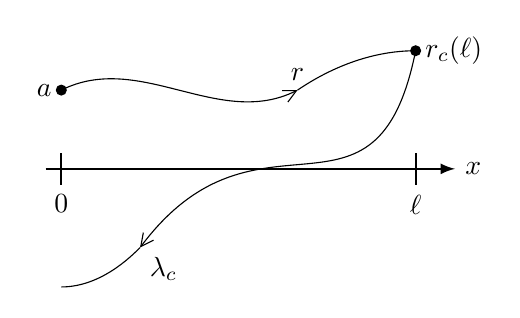
\begin{tikzpicture}
    \draw [thick,->] (-0.2,0) -- (5,0) node [anchor=west] {$x$};
    \draw [thick] (0,0.2) -- (0,-0.2) node [anchor=north] {$0$};
    \draw [thick] (4.5,0.2) -- (4.5,-0.2) node [anchor=north] {$\ell$};
    
    \node [dot] at (0,1) {};
    \node [dot] at (4.5,1.5) {};
    \draw [->,>={Straight Barb[scale length=2]}] (0,1) node [anchor=east] {$a$} .. controls (1,1.5) and (2,0.5) .. (3,1) node [anchor=south] {$r$};
    \draw (3,1) parabola [bend at end] (4.5,1.5) node [anchor=west] {$r_c(\ell)$};

    \draw [->,>={Straight Barb[scale length=2]}] (4.5,1.5) .. controls (4,-1) and (2.5,1) .. (1,-1) node [anchor=north west] {$\lambda_c$};
    \draw (1,-1) parabola [bend at end] (0,-1.5);
  \end{tikzpicture}
\end{center}
Problem: we can do this for any $c$. Which $c$ is it? \emph{Last 15 minutes was a dead end!}

Back to $u=F(r,\lambda)$. Assume we have $F$ (numerically).
\begin{align}
  \frac{\dif r}{\dif x} &= -F(r,\lambda) \\
  r(0) &= a \\
  \frac{\dif\lambda}{\dif x} &= -\frac{F^3(r,\lambda)}{1+F^2(r,\lambda)} \\
  \lambda(\ell) &= r(\ell)
\end{align}
The mistake before was that the simulation forward from $a$ depends on $\lambda$. 
\begin{center}
  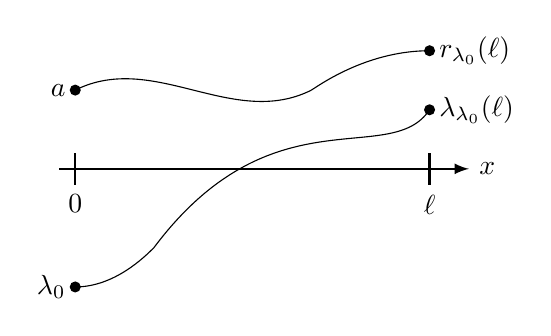
\begin{tikzpicture}
    \draw [thick,->] (-0.2,0) -- (5,0) node [anchor=west] {$x$};
    \draw [thick] (0,0.2) -- (0,-0.2) node [anchor=north] {$0$};
    \draw [thick] (4.5,0.2) -- (4.5,-0.2) node [anchor=north] {$\ell$};
    
    \node [dot] at (0,1) {};
    \node [dot] at (4.5,1.5) {};
    \draw [>={Straight Barb[scale length=2]}] (0,1) node [anchor=east] {$a$} .. controls (1,1.5) and (2,0.5) .. (3,1);
    \draw (3,1) parabola [bend at end] (4.5,1.5) node [anchor=west] {$r_{\lambda_0}(\ell)$};

    \node [dot] at (0,-1.5) {};
    \node [dot] at (4.5,0.75) {};
    \draw [>={Straight Barb[scale length=2]}] (4.5,0.75) node [anchor=west] {$\lambda_{\lambda_0}(\ell)$} .. controls (4,0) and (2.5,1) .. (1,-1);
    \draw (1,-1) parabola [bend at end] (0,-1.5) node [anchor=east] {$\lambda_0$};
  \end{tikzpicture}
\end{center}
Therefore, we should guess $\lambda_0$ and simulate both $r$ and $\lambda$ to get $r_{\lambda_0}(\ell)$ and $\lambda_{\lambda_0}(\ell)$. We need
\[ r_{\lambda_0}(\ell) = \lambda_{\lambda_0} \]
for optimality. To do this, we need numerics.

% 2017/02/09
\paragraph{Terminal Constraints} \mbox{}
\hypertarget{fixed_term_cons}{}

Let $x=[x_1,\dots,x_n]\trans\in\R^n$ and solve
\begin{align}
  & \min_{u\in\mathcal U} \int_0^T L(x,u,t)\dif t + \Psi(x(T)) \\
  & \text{s.t. } \begin{aligned}[t]
    \dot x &= f(x,u,t) \\
    x(0) &= x_0 \\
    x_i(T) &= x_{iT} \quad \text{given for } i\in\mathcal T \subset \{1,\dots,n\}
  \end{aligned}
\end{align}
First, we augment the cost:
\begin{align}
  \tilde J(u) &= \int_0^T \big[ L + \lambda\trans (f-\dot x) \big] \dif t + \Psi \\
              &= \int_0^T (H-\lambda\trans\dot x) \dif t + \Psi \\
  \tilde J (u+\varepsilon v) - \tilde J(u) &= \int_0^T \left( \varepsilon\pder{H}{u} v + \varepsilon\pder{H}{x}\eta - \varepsilon\lambda\trans\dot\eta \right) \dif t + \varepsilon\pder{\Psi}{x}(x(T))\eta(T) + o(\varepsilon) \\
  \delta\tilde J(u;v) &= \int_0^T \left( \pder{H}{x} + \dot\lambda\trans \right)\eta\dif t + \int_0^T \pder{H}{u}v\dif t \\
              & \qquad + \lambda\trans(0)\eta(0) - \lambda\trans(T)\eta(T) + \pder{\Psi}{x}(x(T))\eta(T)
\end{align}
As always,
\begin{align}
  \dot\lambda &= -\pder{H\trans}{x} \\
  \pder{H}{u} &= 0 \quad \text{(FONC)}
\end{align}
Additionally,
\begin{align}
  \eta(0) &= 0 \\
  \eta_i(T) &= 0 \quad \text{for } i\in\mathcal T
\end{align}
Note that if $x(T)=x_T$ is given, then $x(T)=x(T)+\varepsilon\eta(T)+o(\varepsilon)$, so $\eta(T)=0$. Here, we have $x_i(T)=x_{iT}$ fixed for $i\in\mathcal T$ so $\eta_i(T)=0$ for $i\in\mathcal T$.

For optimality, we want
\begin{gather}
  \left[ -\lambda\trans(T) + \pder{\Psi}{x}(x(T)) \right] \eta(T) = 0 \quad \text{for all \emph{admissible} variations} \\
  \begin{bmatrix}
    \displaystyle \pder{\Psi}{x_1}-\lambda_1, & \cdots, & \displaystyle \pder{\Psi}{x_n}-\lambda_n
  \end{bmatrix}
  \begin{bmatrix}
    \eta_1(T) \\
    \vdots \\
    \eta_n(T)
  \end{bmatrix} = 0
\end{gather}
Hence, we need
\begin{alignat}{2}
  \lambda_j(T) &= \pder{\Psi}{x_j}(x(T)) \quad & \text{if } j\not\in\mathcal T \\
  \lambda_i(T) &= \text{free} & \text{if } i\in\mathcal T
\end{alignat}
So we have
\[ \begin{dcases}
    \dot x = f \\
    \dot\lambda = -\pder{H\trans}{x},
  \end{dcases} \]
an ODE with $2n$ variables. We need $2n$ boundary conditions for this ODE to be well-posed.
\begin{center}
  \begin{tabular}{lclc}
    \toprule
    \multicolumn{2}{c}{At $t=0$} & \multicolumn{2}{c}{At $t=T$} \\
    \cmidrule(r){1-2} \cmidrule(l){3-4}
    $x(0)=x_0$ & $[n]$ & $x_i(T)=x_{iT}$, $i\in\mathcal T$ & $[q]$ \\
                                 && $\phantom{x_i(T)=x_{iT}}$ $|\mathcal T|=q$ \\
                                 && $x_j(T)$ free, $j\not\in\mathcal T$ & $[0]$ \\
    $\lambda(0)$ free & $[0]$ & $\lambda_i(T)$ free, $i\in\mathcal T$ & $[0]$ \\
                                 && $\lambda_j(T)=\displaystyle\pder{\Psi}{x_j}(x(T))$, $j\not\in\mathcal T$ & $[n-q]$ \\
    \bottomrule
  \end{tabular}
\end{center}
So we have $n+q+(n-q)=2n$ boundary conditions.

We could even fix some but not all of $x(0)$, i.e.
\begin{alignat}{2}
  x_i(0) &= x_{i0} & \text{if } i\in\mathcal I \\
  x_j(0) &= \text{free} \quad & \text{if } j\not\in\mathcal I
\end{alignat}
Recall,
\[
  \delta\tilde J(u;v) = \int_0^T\! \left(\pder{H}{x} + \dot\lambda\trans \right)\eta\dif t + \int_0^T\! \pder{H}{u} v \dif t + \lambda\trans(0)\eta(0) + \left[\lambda\trans(T)-\pder{\Psi}{x}(x(T))\right] \eta(T)
\]
For $x_i(0)=x_{i0}$ fixed, we have $\eta_i(0)=0$ and $\lambda_i(0)$ free. For $x_j(0)$ free, we have $\eta_j(0)$ free and $\lambda_j(0)=0$.

To ponder, what if $J=\int\! L\dif t + \Psi(x(T)) + \Theta(x(0))$?

To summarize, the minimizer to
\begin{align}
  & \min_{u\in\mathcal U} \int_0^T L(x,u,t)\dif t + \Psi(x(T)) \\
  & \text{s.t. } \begin{aligned}[t]
    \dot x &= f(x,u,t) \\
    x_i(0) &= x_{i0}, \quad i\in\mathcal I \\
    x_j(T) &= x_{jT} \quad j\in\mathcal T
  \end{aligned}
\end{align}
has to satisfy
\begin{align}
  & \pder{H}{u} = 0 \\
  & \dot\lambda = -\pder{H\trans}{x} \\
  & \lambda_i(0) = 0, \quad i\not\in\mathcal I \\
  & \lambda_j(T) = \pder{\Psi}{x_j}(x(T)), \quad j\not\in\mathcal T
\end{align}

\paragraph{Example}
\begin{align}
  & \frac{\dif}{\dif t} \begin{bmatrix}
    x_1 \\ x_2 \\ x_3 \\ x_4
  \end{bmatrix} = f(x_1,x_2,x_3,x_4) \\
  & x_1(0)=1,\, x_3(0)=7,\, x_4(0)=0,\, x_1(1)=2 \\
  & \mathcal I = \{1,3,4\},\, \mathcal T = \{1\} \\
  & \min \int_0^1 L(x,u)\dif t + \big(x_2^2(1) - x_3^2(1) + 7x_1(1) + 14 \big)
\end{align}
Note there are 4 boundary conditions on $x$ so there must be 4 boundary conditions on $\lambda$:
\begin{alignat}{4}
  & \lambda_1(0) \text{ free/unspecified} & \qquad & \lambda_1(1) \text{ free} \\
  & \lambda_2(0) = 0 && \lambda_2(1) = 2x_2(1) \\
  & \lambda_3(0) \text{ free} && \lambda_3(1) = -2x_3(1) \\
  & \lambda_4(0) \text{ free} && \lambda_4(1) = 0
\end{alignat}

\paragraph{Example} \mbox{}

A force $f$ acts on a particle at position $(x,y)$ ($\text{mass}=1$).

\begin{center}
  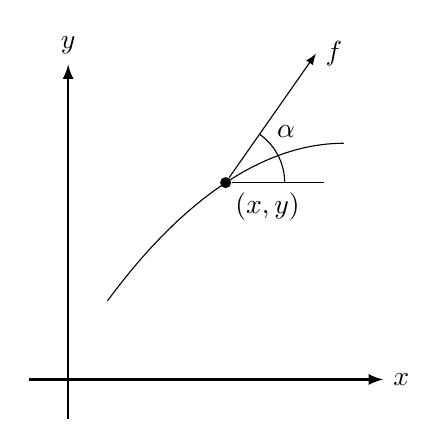
\begin{tikzpicture}
    \draw [thick,->] (-0.5,0) -- (4,0) node [anchor=west] {$x$};
    \draw [thick,->] (0,-0.5) -- (0,4) node [anchor=south] {$y$};
    \draw (0.5,1) parabola [bend at end] (3.5,3);
    \node [dot] (x) at (2,2.5) {};
    \node [anchor=north west] at (x) {$(x,y)$};
    \draw [->] (x) -- ++(55:2) node [anchor=west] {$f$};
    \draw ($(x)+(55:0.75)$) arc (55:0:0.75);
    \node at ($(x)+(40:1)$) {$\alpha$};
    \draw (x) -- ++(1.25,0);
  \end{tikzpicture}
\end{center}
\begin{align}
  \dot x &= v_x \\
  \dot y &= v_y \\
  \dot v_x &= |f|\cos\alpha \\
  \dot v_y &= |f|\sin\alpha \\
  \alpha &= \text{control variable}
\end{align}
Assume we only care about where the particle ends up (to be specified later), i.e.\ $L=0$.
\[
  H = \begin{bmatrix}
    \lambda_x & \lambda_y & \lambda_{v_x} & \lambda_{v_y}
  \end{bmatrix}
  \begin{bmatrix}
    v_x \\ v_y \\ |f|\cos\alpha \\ |f|\sin\alpha
  \end{bmatrix}
\]
\begin{alignat}{3}
  \dot\lambda_x &= -\pder{H}{x} = 0 && \Longrightarrow & \lambda_x(t) &= c_1 \\
  \dot\lambda_y &= -\pder{H}{y} = 0 && \Longrightarrow & \lambda_y(t) &= c_2 \\
  \dot\lambda_{v_x} &= -\pder{H}{v_x} = -\lambda_x && \Longrightarrow & \lambda_{v_x}(t) &= -c_1 t + c_3 \\
  \dot\lambda_{v_y} &= -\pder{H}{v_y} = -\lambda_y \quad && \Longrightarrow & \quad \lambda_{v_y}(t) &= -c_2 t + c_4
\end{alignat}
Moreover,
\begin{align}
  \pder{H}{\alpha} &= -\lambda_{v_x} |f| \sin\alpha + \lambda_{v_y} |f| \cos\alpha = 0 \\
  \tan\alpha &= \frac{\lambda_{v_y}}{\lambda_{v_x}} = \frac{-c_2t+c_4}{-c_1t+c_3}
\end{align}
We want to drive the particle from $[0,0,0,0]\trans$ to a path parallel to the x-axis with $y(T)=h$.

\begin{center}
  \begin{tikzpicture}
    \draw [thick,->] (-0.5,0) -- (5.5,0) node [anchor=west] {$x$};
    \draw [thick,->] (0,-0.5) -- (0,3) node [anchor=south] {$y$};
    \draw [thick] (0.2,2) -- (-0.2,2) node [anchor=east] {$h$};
    \draw (0,0) parabola [bend at end] (3.5,2) -- ++(0.5,0) coordinate (x);
    \node [dot] at (x) {};
    \node [anchor=south] at (x) {$t=T$};
  \end{tikzpicture}
\end{center}
Choose $\Psi=-v_x$,
\begin{alignat}{2}
  y(T) &= h & v_y(T) &= 0 \\
  x(T) & \text{ free} \quad & v_x(T) &\phantom{x} \text{free, but costs} \\
  \lambda_i(0) & \text{ free} \\
  \lambda_y(T) & \text{ free} & \lambda_{v_y}(T) & \text{ free} \\
  \lambda_x(T) &= 0 & \lambda_{v_x}(T) &= -1
\end{alignat}
\begin{align}
  c_1 &= \lambda_x(t) = 0 \\
  \Longrightarrow \lambda_{v_x} &= -c_1t + c_3 = c_3 = -1 \\
  \Longrightarrow \tan\alpha &= -\frac{-c_2t+c_4}{-1} = c_2t + c_4
\end{align}
How do we find $c_2$ and $c_4$? Plug into $\dot x$ and $\dot\lambda$ and try to satisfy the remaining boundary conditions. (This is hard=numerics.)

% 2017/02/14
\section{Splines}
\emph{From ship building.}
Splines are used a lot in path-planning, e.g. cubic splines.
\begin{center}
  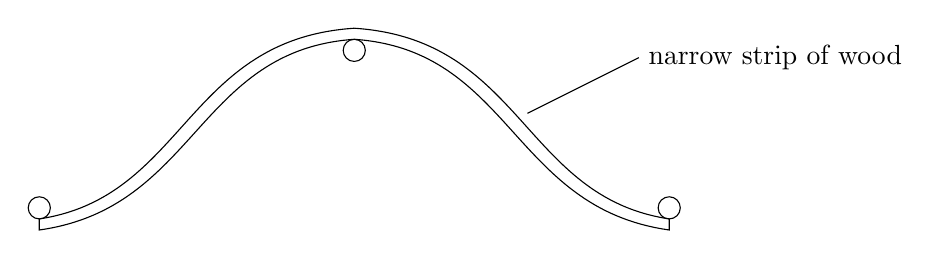
\begin{tikzpicture}[x=2cm,y=1cm]
    \draw (0,0) circle (4pt);
    \draw (2,2) circle (4pt);
    \draw (4,0) circle (4pt);
    \draw ([yshift=-4pt]0,0) .. controls ([xshift=-4pt,yshift=4pt]1,0) and ([xshift=-4pt,yshift=4pt]1,2) .. ([yshift=8pt]2,2);
    \draw ([yshift=-4pt]0,0) -- ([yshift=-8pt]0,0) .. controls (1,0) and (1,2) .. ([yshift=4pt]2,2);
    \draw ([yshift=-4pt]4,0) -- ([yshift=-8pt]4,0) .. controls (3,0) and (3,2) .. ([yshift=4pt]2,2);
    \draw ([yshift=-4pt]4,0) .. controls ([xshift=4pt,yshift=4pt]3,0) and ([xshift=4pt,yshift=4pt]3,2) .. ([yshift=8pt]2,2);
    \draw (3.1,1.2) -- ++(45:1) node [anchor=west] {narrow strip of wood};
  \end{tikzpicture}
\end{center}
But, they are solutions to optimal control problems.

Let $p(t)$ be a curve we'd like to shape.
\pgfmathsetseed{11}
\begin{center}
  \begin{tikzpicture}
    \def\x{0.4}
    \def\dy{0.3}
    \draw [->,thick] (-0.5,0) -- (5,0) node [anchor=west] {$t$};
    \draw [->,thick] (0,-0.5) -- (0,3);
    \draw (0,1) sin (\x,1+\dy) cos (2*\x,1) sin (3*\x,1-\dy) cos (4*\x,1)
    sin (5*\x,1+\dy) cos (6*\x,1) sin (7*\x,1-\dy*2/3) cos (9*\x,1+\dy*2)
    sin (10*\x,1+\dy*3) cos (10.5*\x,1+\dy*2.7) node [anchor=west] {$p(t)$};
  \end{tikzpicture}
\end{center}
We want to minimize the ``energy'' put into the curve, a.k.a\ acceleration.
Let $x_1=p$ and $x_2=\dot p$, so
\[ \begin{cases}
    \dot x_1 = x_2 \\
    \dot x_2 = u
  \end{cases} \]

\subsection{Minimum-Energy}

\begin{align}
  & \min_{u\in\mathcal U} \frac{1}{2} \int_0^T u^2(t)\dif t \quad \text{+ Boundary conditions on $x$} \\
  H &= L+\lambda\trans f = \frac12 u^2 + \lambda_1 x_2 + \lambda_2 u \\
  \pder{H}{u} &= u + \lambda_2 = 0 \Longrightarrow u = -\lambda_2 \\
  \dot\lambda_1 &= -\pder{H}{x_1} = 0 \Longrightarrow \lambda_1 = c_1 \\
  \dot\lambda_2 &= -\pder{H}{x_2} = -\lambda_1 \Longrightarrow \lambda_2 = -c_1t+c_2 \\
  u &= -\lambda_2 = c_1t-c_2 \\
  \dot x_2 &= u = c_1t-c_2 \Longrightarrow x_2 = c_1 \frac{t^2}{2} - c_2t + c_3 \\
  \dot x_1 &= x_2 = c_1\frac{t^2}{2} -c_2t + c_3 \\
  & \Longrightarrow x_1 = \frac{c_1}{6}t^3 - \frac{c_2}{2}t^2 + c_3 t + c_4
\end{align}
$p(t)$ is a cubic polynomial!

\medskip \noindent
What about boundary conditions?

Let $T=1$, $p(0)$ given, $p(1)$ given, $\dot p(0)=0$, $\dot p(1)=0$, e.g.\ $p(0)=0$, $p(1)=1$. Since the boundary conditions for $x$ are all specified, those for the costate are free.
\[
  \left.
    \begin{aligned}
      x_1(0) &= 0 \\
      x_2(0) &= 0 \\
      x_1(1) &= 1 \\
      x_2(1) &= 0
    \end{aligned} \right\}
  \Longrightarrow
  \left\{
    \begin{aligned}
      \lambda_1(0) \\
      \lambda_2(0) \\
      \lambda_1(1) \\
      \lambda_2(1)
    \end{aligned} \right.
  \quad \text{free/unspecified}
\]
\begin{alignat}{2}
  x_2(0) &= c_3 = 0 & x_1(1) &= \frac{2c_2}{6} - \frac{c_2}{2} = 1 \\
  x_1(0) &= c_4 = 0 & c_2 &= -6 \\
  x_2(1) &= \frac{c_1}{2} - c_2 + \smash{ \underbrace{c_3}_{0} } = 0 & c_1 &= -12 \\
  c_1 &= 2c_2
\end{alignat}
\begin{align}
  \Longrightarrow \; & p(t) = -2t^3 + 3t^2 \\
                     & u(t) = -12t + 6
\end{align}

Or, what if $\dot p(0)$, $\dot p(1)$ are not specified?
\[
  \left.
    \begin{aligned}
      x_1(0) &= 0 \\
      x_2(0) & \text{ unspec.} \\
      x_1(1) &= 1 \\
      x_2(1) & \text{ unspec.}
    \end{aligned} \right\}
  \Longrightarrow
  \left\{
    \begin{aligned}
      & \lambda_1(0) \text{ unspec.} \\
      & \lambda_2(0) = 0 \\
      & \lambda_1(1) \text{ unspec.} \\
      & \lambda_2(1) = 0
    \end{aligned} \right.
\]
\begin{align}
  \left.
  \begin{aligned}
    \lambda_2(0) &= c_2 = 0 \\
    \lambda_2(1) &= -c_1 + c_2 = 0
  \end{aligned}
                   \right\} & \Longrightarrow
                              u = c_1t- c_2 = 0 \\
  \left.
  \begin{aligned}
    x_1(0) = c_4 = 0 \\
    x_1(1) = c_3 = 1
  \end{aligned}
  \right\} & \Longrightarrow
             p(t) = t
\end{align}

\noindent
What did we do?
\begin{enumerate}[label=Case \arabic*:,itemindent=1cm]
\item \mbox{}
  \begin{gather}
    \begin{bmatrix}
      0 & 0 & 0 & 1 \\
      1/6 & -1/2 & 1 & 1 \\
      0 & 0 & 1 & 0 \\
      1/2 & -1 & 1 & 0
    \end{bmatrix}
    \begin{bmatrix}
      c_1 \\ c_2 \\ c_3 \\ c_4
    \end{bmatrix}
    =
    \begin{bmatrix}
      0 \\ 1 \\ 0 \\ 0
    \end{bmatrix}
    =
    \begin{bmatrix}
      x_1(0) \\ x_1(1) \\ x_2(0) \\ x_2(1)
    \end{bmatrix}
  \end{gather}
\item \mbox{}
  \begin{gather}
    \begin{bmatrix}
      0 & 0 & 0 & 1 \\
      1/6 & -1/2 & 1 & 1 \\
      0 & 1 & 0 & 0 \\
      -1 & 1 & 0 & 0
    \end{bmatrix}
    \begin{bmatrix}
      c_1 \\ c_2 \\ c_3 \\ c_4
    \end{bmatrix}
    =
    \begin{bmatrix}
      0 \\ 1 \\ 0 \\ 0
    \end{bmatrix}
    =
    \begin{bmatrix}
      x_1(0) \\ x_1(1) \\ \lambda_2(0) \\ \lambda_2(1)
    \end{bmatrix}
  \end{gather}
\end{enumerate}

\subsection{Generalized Splines}
We had $\dot x=Ax+Bu$ with
\[ A = \begin{bmatrix}
    0 & 1 \\ 0 & 0
  \end{bmatrix}. \]
This $A$ is nilpotent ($A^k=0$ for some $k\in\mathbb Z^+$). This means $e^{At}$ is a polynomial in $t$. (This $e^{At}$ is cubic.)

In general, $e^{At}$ is a mix of polynomials, exponentials, and trignometric terms. The eigenvalues of $A$ determine the form of $x(t)$.
\begin{alignat}{3}
  \dot x &= Ax && \Longrightarrow & \; x(t) &= e^{At} x(0) \\
  \dot x &= Ax + Bu && \Longrightarrow & x(t) &= e^{At} x(0) + \int_0^t e^{A(t-\tau)} Bu(\tau) \dif\tau
\end{alignat}
The general problem to solve is
\begin{align}
  & \min_{u\in\mathcal U} \int_0^T \frac{1}{2} \Vert u\Vert^2 \dif t \\
  & \text{s.t. } \dot x = Ax + Bu \\
  & \quad \text{+ Boundary conditions}
\end{align}
\begin{align}
  H &= \frac{1}{2} \Vert u\Vert^2 + \lambda\trans (Ax+Bu) \\
  \pder{H}{u} &= u\trans + \lambda\trans B = 0 \\
    & \Rightarrow u = -B\trans\lambda \\
  \dot\lambda &= -\pder{H\trans}{x} = -A\trans\lambda
\end{align}
We have the Hamiltonian Dynamics:
\begin{gather}
  \begin{bmatrix}
    \dot x \\ \dot\lambda
  \end{bmatrix} =
  \underbrace{
      \begin{bmatrix}
        A & -BB\trans \\
        0 & -A\trans
      \end{bmatrix}
  }_{M}
  \begin{bmatrix}
    x \\ \lambda
  \end{bmatrix}
\end{gather}
Where we used $\dot x=Ax+Bu=Ax-BB\trans\lambda$. Then,
\begin{gather}
  \begin{bmatrix}
    x(t) \\ \lambda(t)
  \end{bmatrix} =
  e^{Mt}
  \begin{bmatrix}
    x(0) \\ \lambda(0)
  \end{bmatrix}
\end{gather}
Suppose we want to drive from $x(0)=x_0$ to $x(T)=x_T$.
\begin{gather}
  \begin{bmatrix}
    x_T \\ \lambda(T)
  \end{bmatrix} =
  e^{MT}
  \begin{bmatrix}
    x_0 \\ \lambda(0)
  \end{bmatrix} =
  \begin{bmatrix}
    N_{xx} & N_{x\lambda} \\
    N_{\lambda x} & N_{\lambda\lambda}
  \end{bmatrix}
  \begin{bmatrix}
    x_0 \\ \lambda(0)
  \end{bmatrix} \\
  x_T = N_{xx} x_0 + N_{x\lambda} \lambda(0) \\
  \intertext{$N_{x\lambda}$ is invertible if $(A,B)$ is completely controllable. Assume it is.}
  \lambda(0) = N_{x\lambda}^{-1} (x_T - N_{xx} x_0) \\
  \Longrightarrow
  \begin{bmatrix}
    x(t) \\ \lambda(t)
  \end{bmatrix} =
  e^{Mt}
  \begin{bmatrix}
    x_0 \\
    N_{x\lambda}^{-1} (x_T - N_{xx} x_0)
  \end{bmatrix} \\
  \Longrightarrow u(t) = -B\trans \lambda(t)
\end{gather}
This is the optimal trajectory, but there is no feedback. We will consider closed-loop systems after the midterm.

As a preview, we need to find $\lambda$ as a function of $x$. For example, $u=-R^{-1} B\trans Px$ minimizes $u\trans Ru$, so $\lambda=Px$ where $P$ is the solution to the Riccati equation.

% 2017/02/16
\section{Numerical Methods}
Optimal control boils down to solving two sets of differential equations:
\begin{gather}
  \begin{aligned}
    \dot x &= f(x,u) & \quad & \pder{H}{u}(x,u,\lambda) = 0 \\
    \dot\lambda &= -\pder{H\trans}{x}(x,u,\lambda) && u = F(x,\lambda) \\
  \end{aligned} \\
  \Longrightarrow \begin{dcases}
    \dot x = f(x,F(x,\lambda)) \\
    \dot \lambda = -\pder{H\trans}{x}(x,F(x,\lambda),\lambda)
  \end{dcases}
\end{gather}
The equations are functions of $x$ and $\lambda$. They are completely determined by the boundary conditions on $x(0)$, $x(T)$, $\lambda(0)$, $\lambda(T)$. This is known as the \emph{Boundary Value Problem}. This is solved using \emph{test shooting}:
\begin{enumerate}
\item Guess initial conditions
\item Simulate forward in time
\item Update the guess (cleverly\dots)
\end{enumerate}

\paragraph{Exmaple:} Bolza problem
\begin{align}
  & \min_{u\in\mathcal U} \int_0^T L(x,u)\dif t + \Psi(x(T)) \\
  & \text{s.t. } \begin{cases}
    \dot x=f(x,u) \\
    x(0) = x_0
  \end{cases} \\
  & H(x,u,\lambda) = L(x,u) + \lambda\trans f(x,u) \\
  & u^* (x,\lambda) \text{ satisfies } \pder{H}{u} = 0
\end{align}
The optimal control satisfies
\begin{gather}
  \begin{dcases}
    x = f(x,u^*(x,\lambda)) \\
    x(0) = x_0 \\
    \lambda = -\pder{H\trans}{x} (x,u^*(x,\lambda),\lambda) \\
    \lambda(T) = \pder{\Psi}{x}(x(T))
  \end{dcases}
\end{gather}

\paragraph{Algorithm}
Guess $\lambda_0$ and solve for $x(t)$, $\lambda(t)$.
\begin{center}
  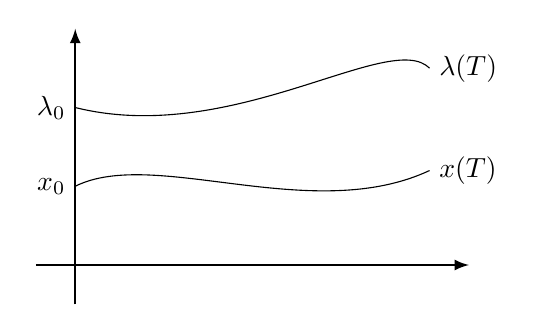
\begin{tikzpicture}
    \draw [thick,->] (-0.5,0) -- (5,0);
    \draw [thick,->] (0,-0.5) -- (0,3);
    \draw (0,1) node [anchor=east] {$x_0$} .. controls (1,1.5) and (3,0.5) .. (4.5,1.2) node [anchor=west] {$x(T)$};
    \draw (0,2) node [anchor=east] {$\lambda_0$} .. controls (2,1.5) and (4,3) .. (4.5,2.5) node [anchor=west] {$\lambda(T)$};
  \end{tikzpicture}
\end{center}
Let's define a cost:
\[ \left\Vert \lambda(T) - \pder{\Psi\trans}{x}(x(T)) \right\Vert^2 = g(\lambda_0) \]
Update $\lambda_0$ through
\[ \lambda_0 \coloneqq \lambda_0 - \underset{\mathclap{\substack{\big\uparrow\\ \text{\normalsize any choice of step size works}}}}{\gamma} \pder{g\trans}{\lambda_0}(\lambda_0) \]
Repeat

\medskip

\noindent
Problem: What is $\partial g/\partial\lambda_0$? We estimate $\partial g/\partial\lambda_0$ numerically. This is where ``test shooting'' comes into play.

Let $e_i$ be the $i$th unit vector, $i=1,\dots,n$:
\begin{gather}
  e_1 = \begin{bmatrix}
    1 \\ 0 \\ \vdots \\ 0
  \end{bmatrix}\!,\ 
  e_2 = \begin{bmatrix}
    0 \\ 1 \\ \vdots \\ 0
  \end{bmatrix}\!,\ 
  \dots,\ 
  e_n = \begin{bmatrix}
    0 \\ 0 \\ \vdots \\ 1
  \end{bmatrix} \\
  \pder{g}{\lambda_0} = \left( \pder{g}{\lambda_{0,1}},\pder{g}{\lambda_{0,2}},\dots,\pder{g}{\lambda_{o,n}} \right)
\end{gather}
The $i$th component of $\partial g/\partial\lambda_0$ is given by the directional derivative
\[
  \pder{g}{\lambda_{0,i}} = \pder{g}{\lambda_0} \cdot e_i = \delta g(\lambda_0;e_i) = \lim_{\varepsilon\to0} \frac{g(\lambda_0+\varepsilon e_i) - g(\lambda_0)}{\varepsilon}
\]
So, if $x\in\R^n$ (and thus so is $\lambda_0$), we have to do this $n$ times (with a small $\varepsilon$) and get the full derivative $\partial g/\partial\lambda_0$.

\paragraph{Algorithm} \mbox{}
\begin{algorithm}
  \begin{algorithmic}
    \State Given $\lambda_0$, $g(\lambda_0)$
    \For {$i=1$ to $n$}
    \State Compute $g(\lambda_0+\varepsilon e_i)$
    \State $dg_i = \dfrac{1}{\varepsilon} [g(\lambda_0+\varepsilon e_i) - g(\lambda_0)]$
    \EndFor
    \smallskip
    \State $\displaystyle\pder{g}{\lambda_0} = [dg_1,\dots,dg_n]$
  \end{algorithmic}
\end{algorithm}

\paragraph{Example} LQ
\begin{align}
  & \min_u \frac12 \int_0^1 (x\trans Qx + u\trans Ru) \dif t + \frac12 x\trans(1)Sx(1) \\
  & \text{s.t. } \begin{dcases}
    \dot x = Ax + Bu \\
    x(0) = x_0
  \end{dcases} \\
  & \phantom{\text{s.t. }} Q,R,S \succ 0
\end{align}
\begin{align}
  H &= \frac12 x\trans Qx + \frac12 u\trans Ru + \lambda\trans(Ax+Bu) \\
  \pder{H}{u} &= u\trans R + \lambda\trans B = 0 \\
  u^* &= -R^{-1}B\trans \lambda \\
  \dot\lambda &= -\pder{H\trans}{x} = -Qx - A\trans\lambda \\
  \lambda(1) &= \pder{\Psi\trans}{x}(x(1)) = Sx(1)
\end{align}
So putting it all together,
\begin{alignat}{2}
  \dot x &= Ax - BR^{-1}B\trans\lambda \qquad & x(0) &= x_0 \\
  \dot\lambda &= -Qx - A\trans\lambda & \lambda(1) &= Sx(1)
\end{alignat}

\paragraph{Example} Newton's nose shape problem (\hyperlink{newton_nose_shape}{revisited, see previous})

\begin{align}
  & \min_u \int_0^\ell \frac{ru^3}{1+u^2}\dif x + \frac12 r(\ell)^2 \\
  & \text{s.t. } \frac{\dif r}{\dif x} = -u \qquad r(0) = a
\end{align}
\begin{align}
  H &= \frac{ru^3}{1+u^2} + \lambda(-u) \\
  \pder{H}{u} &= \frac{ru^2(3+u^2)}{(1+u^2)^2} - \lambda = 0 \\
  \shortintertext{We solve the above numerically to get $u^*(r,\lambda)$.}
  \pder{\lambda}{x} &= -\pder{H}{r} = -\frac{u^3}{1+u^2} \\
  \lambda(\ell) &= r(\ell)
\end{align}
So, we have
\begin{alignat}{3}
  \frac{\dif r}{\dif x} &= -u & r(0) &= a & u &= F(x,\lambda) \\
  \frac{\dif\lambda}{\dif x} &= -\frac{u^3}{1+u^2} \qquad & \lambda(\ell) &= r(\ell) \qquad
\end{alignat}

\paragraph{Example} Fixed terminal constraints (\hyperlink{fixed_term_cons}{revisited, see previous})

\begin{align}
  & \min_\alpha -v_x(T) \qquad \alpha=\text{control} \\
  & \text{s.t. } \begin{aligned}[t]
    \dot x &= v_x & x(0) &= 0 \\
    \dot y &= v_y & y(0) &= 0 \\
    \dot v_x &= |f|\cos\alpha & v_x(0) &= 0 \\
    \dot v_y &= |f|\sin\alpha & v_y(0) &= 0 \\
    y(T) &= h \\
    v_y(T) &= 0
  \end{aligned}
\end{align}
\begin{align}
  H &= -v_x(T) + \begin{bmatrix}
    \lambda_x & \lambda_y & \lambda_{v_x} & \lambda_{v_y}
  \end{bmatrix}
                                            \begin{bmatrix}
                                              v_x \\ v_y \\ |f|\cos\alpha \\ |f|\sin\alpha
                                            \end{bmatrix} \\
  \frac{\dif H}{\dif\alpha} &= 0 \Rightarrow \tan\alpha = \frac{\lambda_{v_y}}{\lambda_{v_x}} \\
  \dot\lambda_x &= 0 \\
  \dot\lambda_y &= 0 \\
  \dot\lambda_{v_x} &= -\lambda_x \\
  \dot\lambda_{v_y} &= -\lambda_y \\
  \bm\lambda(0) & \text{ unspecified} \\
  \lambda_x(T) &= \pder{\Psi\trans}{x}(x(T)) = 0 \\
  \lambda_y(T) & \text{ unspecified} \\
  \lambda_{v_x}(T) &= \pder{\Psi\trans}{v_x}(v_x(T)) = -1 \\
  \lambda_{v_y}(T) & \text{ unspecified}
\end{align}
Again, we guess $\lambda_0$ and solve forward in time. But, we have terminal constraints on $y$ and $v_y$ as well.
\begin{gather}
  g(\lambda_0) = \frac12 \Big[ (y(T)-h)^2 + (v_y(T))^2 + (\lambda_x(T))^2 + (\lambda_{v_x}+1)^2 \Big]
\end{gather}

% 2017/02/28

\section{Terminal Manifolds}

We can solve
\begin{align}
  & \min_{u\in\mathcal U} \int_0^T L(x,u,t)\dif t + \Psi(x(T)) \\
  & \text{s.t. } \dot x = f(x,u,t)
\end{align}
with all sorts of boundary conditions on $x$:
\begin{itemize}
\item $x(0)=x_0$, $x(T)$ free (typical)
\item $x_i(0)=x_{i0}$, $i\in\mathcal I$ and $x_j(T)=x_{jT}$, $j\in\mathcal T$
\end{itemize}
But what if we want $x(T)$ to belong to a set?

\begin{center}
  \begin{tikzpicture}
    \draw (0,0) coordinate (a) .. controls (1.5,0.5) and (2,-0.5) .. (4,-1) coordinate (b);
    \node [dot] at (a) {};
    \node [dot] at (b) {};
    \node [below left] at (a) {$x_0$};
    \node [right] at (b) {$x(T)$};
    \draw (b) arc (-160:200:0.75cm and 1.25cm);
    \node [right] at ($(b)+(1.5,0.5)$) {$\phi=0$};
  \end{tikzpicture}
\end{center}

\paragraph{Problem}
\begin{align}
  & \min_{u\in\mathcal U} \int_0^T L(x,u,t)\dif t + \Psi(x(T)) \\
  & \text{s.t. } \begin{aligned}[t]
    & \dot x = f(x,u,t), && x\in\R^n \\
    & x(0) = x_0 \\
    & \phi(x(T)) = 0, && \phi:\R^n\to\R^q,\ q\le n
  \end{aligned}
\end{align}
The augmented cost is
\[
  \tilde J = \int_0^T [ H(x,u,t,\lambda) - \lambda\trans \dot x]\dif t + \Psi(x(T)) + \underset{\mathclap{\substack{\uparrow\\ \text{q-dimensional}\\ \text{Lagrange multiplier}}}}{\nu}\trans \phi(x(T))
\]
Let $\Phi(x(T),\nu)=\Psi(x(T)) + \nu\trans\phi(x(T))$. Then,
\[
  \tilde J = \int_0^T \left( \pder{H}{x} + \dot\lambda\trans \right) \eta \dif t + \Phi(x(T),\nu)
\]
We know how to solve this! With $u\mapsto u+\varepsilon v$, $x\mapsto x+\varepsilon\eta + o(\varepsilon)$,
\begin{align}
  \delta \tilde J &= \int_0^T \left(\pder{H}{x} + \dot\lambda\trans\right)\eta\dif t + \int_0^T \pder{H}{u}v \dif t + \pder{\Phi}{x}(x(T),\nu)\eta(T) \\
                  & \qquad - \lambda\trans(T)\eta(T) + \lambda\trans(0)\underbracket{\eta(0)}_{=0} \\
                  & \begin{dcases}
                    \pder{H}{u} = 0 \\
                    \dot\lambda = -\pder{H\trans}{x} \\
                    \lambda(T) = \pder{\Phi\trans}{x}( x(T), \overset{\mathclap{\substack{q \text{ new variables}\\ \downarrow}}}{\nu} ) \\
                    \phi(x(T)) = 0 \ \leftarrow q \text{ new equations}
                  \end{dcases} \\
                  & \Longrightarrow u^*
\end{align}

\paragraph{Spling to line}

\begin{align}
  & \min_u \frac12 \int_0^1 u^2(t) \dif t \\
  & \text{s.t. } \adjustbox{valign=t}{$\begin{dcases}
        \dot x_1 = x_2 \\
        \dot x_2 = u \\
        x_1(0) = 0,\ x_2(0) = 0 \\
        c_1 x_1(1) + c_2 x_2(1) = d
      \end{dcases}$}
\end{align}

\begin{center}
  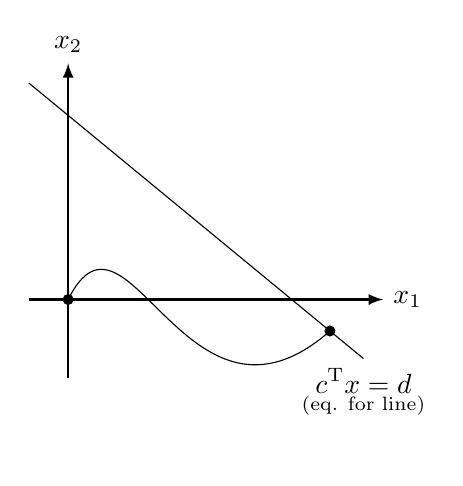
\begin{tikzpicture}
    \draw [thick,->] (-0.5,0) -- (4,0) node [right] {$x_1$};
    \draw [thick,->] (0,-1) -- (0,3) node [above] {$x_2$};
    \draw (-0.5,2.75) coordinate (a) -- (3.75,-0.75) coordinate (b) node [below] {$\substack{\displaystyle c\trans x=d\\ \text{(eq. for line)}}$};
    \draw (0,0) coordinate (o) .. controls (0.75,1.5) and (1.5,-2) .. ($(b)!0.1!(a)$) coordinate (c);
    \node [dot] at (o) {};
    \node [dot] at (c) {};
  \end{tikzpicture}
\end{center}

\begin{align}
  H &= \frac12 u^2 + \lambda_1 x_2 + \lambda_2 u \\
  \pder{H}{u} &= u + \lambda_2 \Longrightarrow u = -\lambda_2 \\
  \dot\lambda_1 &= -\pder{H}{x_1} = 0 \Longrightarrow \lambda_1 = k_1 \\
  \dot\lambda_2 &= -\pder{H}{x_2} = -\lambda_1 \Longrightarrow \lambda_2 = -k_1 t + k_2 \\
  \phi(x(1)) &= c_1 x_1(1) + c_2 x_2(1) - d \\
  \Psi &= 0 \Longrightarrow \Phi = \nu (c_1x_1(1) + c_2x_2(1) - d) \\
  \lambda_1(1) &= \pder{\Phi}{x_1} = \nu c_1 \\
  \lambda_2(1) &= \pder{\Phi}{x_2} = \nu c_2 \\
  \shortintertext{So,}
  \lambda_1(1) &= \nu c_1 = k_1 \\
  \lambda_2(1) &= \nu c_2 = -k_1 + k_2 \\
  k_2 &= \nu (c_1 + c_2) \\
  \dot x_2 &= u = -\lambda_2 = k_1 t - k_2 \\
  x_2 &= \frac{k_1}{2} t^2 - k_2 t + 0 \\
  \dot x_1 &= x_2 \\
  x_1 &= \frac{k_1}{6} t^3 - \frac{k_2}{2} t^2 + 0 \\
  \shortintertext{Substituting $k_1$ and $k_2$ into $c_1x_1(1)+c_2x_2(1)=d$,}
    & \nu \left( -\frac{c_1^2}{3} - c_1 c_2 - c_2^2 \right) = d \\
  \nu &= - \frac{d}{c_1^2/3 + c_1c_2 + c_2^2} \\
  \shortintertext{And finally}
  \Aboxed{u &= k_1 t - k_2 = \frac{d}{c_1^2/3 + c_1c_2 + c_2^2} (c_1 + c_2 - c_1 t)}
\end{align}
As a final observation if $\Psi=0$ then
\[
  \lambda(T) = \nu\trans \pder{\phi}{x}(x(T)),
\]
which means $\lambda(T)$ is orthogonal to the tangent plane to $\phi(x(T))$.

\begin{center}
  \begin{tikzpicture}
    \draw (0,0) parabola [bend at end] (1,0.5);
    \draw (1,0.5) parabola (3,-2);
    \draw (3,-2) parabola [bend at end] (3.5,-2.5);
    \draw (3.5,-2.5) -- ++(3,0) node [right] {$\phi=0$};
    \draw [->] (5,-2.5) coordinate (a) -- ++(0,-1.25) coordinate (b);
    \node [below] at (b) {$\lambda(T)$};
    \draw ($(a)!8pt!(b)$) coordinate (c) -- ($(c)!1!-90:(a)$) coordinate (d);
    \draw (d) -- ($(d)!1!-90:(c)$);
    \draw [->] (2.25,-0.48) coordinate (e) -- ++ (33:1.25) coordinate (f);
    \node [right] at (f) {$\lambda(T)$};
    \draw ($(e)!8pt!(f)$) coordinate (g) -- ($(g)!1!90:(e)$) coordinate (h);
    \draw (h) -- ($(h)!1!90:(g)$);
  \end{tikzpicture}
\end{center}

\paragraph{Example} Maximum orbit transform (e.g.\ Hidden Figures)

\bigskip

\begin{tabular}{cc}
  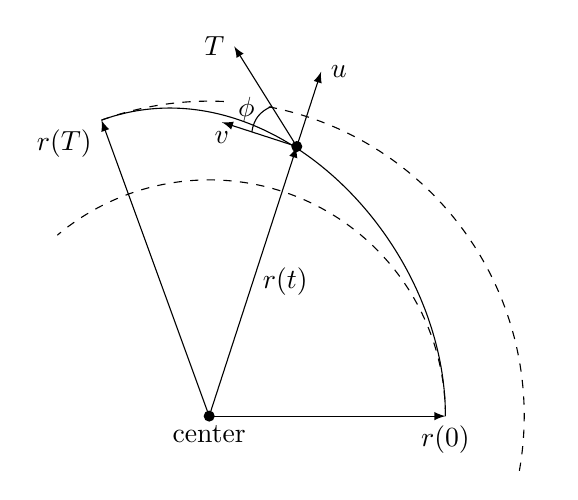
\begin{tikzpicture}[baseline=(c)]
    \node [dot] at (0,0) {};
    \node [below] at (0,0) {center};
    \draw [->] (0,0) -- ++(3,0) coordinate (a);
    \node [below] at (a) {$r(0)$};
    \draw [->] (0,0) -- ++(110:4) coordinate (b);
    \node [below left] at (b) {$r(T)$};
    \draw (a) to [out=90,in=20] (b);
    \draw [dashed] (a) arc (0:130:3);
    % \draw [dashed] (b) arc (110:-10:4);
    \path (b) arc (110:-10:4) coordinate (rT);
    \draw [dashed] (b) arc (110:86:4);
    \draw [dashed] (rT) arc (-10:80:4);

    \draw [->] (0,0) -- ++(72:3.6) coordinate (c) node [pos=0.5,right] {$r(t)$};
    \node [dot] at (c) {};
    \draw [->] (c) -- ($(c)!-1cm!(0,0)$) coordinate (u);
    \node [right] at (u) {$u$};
    \draw [->] (c) -- ($(c)!1!90:(u)$) coordinate (v) node [below] {$v$};
    \draw [->] (c) -- ($(c)!1.5!50:(u)$) coordinate (T) node [left] {$T$};
    \path ($(c)!0.6cm!(v)$) coordinate (vv) ($(c)!0.6cm!(T)$) coordinate (TT);
    \draw (vv) to [bend left] (TT);
    \node [above,xshift=-2pt] at (vv) {$\phi$};
  \end{tikzpicture}
  &
    \begin{tabular}[t]{>{$}r<{$} @{${}={}$} p{6cm}}
      r & radial distance from spacecraft to center \\
      u & radial velocity \\
      v & tangential velocity \\
      m & mass of spacecraft \\
      \dot m & $-$fuel consumption rate \\
      \phi & thrust angle (control input) \\
      T & thrust
    \end{tabular}
\end{tabular}

\begin{align}
  & \max_\phi r(T) \Longleftrightarrow \min_\phi -r(T) \\
  & \text{s.t. } \adjustbox{valign=t}{$\begin{dcases}
        \dot r = u \\
        \dot u = \frac{v^2}{r} - \frac{g}{r^2} + \frac{T\sin\phi}{m_0 - |\dot m|t} \\
        \dot v = -\frac{uv}{r} + \frac{T\cos\phi}{m_0 - |\dot m|t} \\
        r(0) = r_0 \\
        u(0) = 0 \\
        v(0) = \sqrt{\frac{g}{r_0}} \\
        u(T) = 0 = \phi_1 \\
        v(T) = \sqrt{\frac{g}{r(T)}} = \phi_2
      \end{dcases}$}
\end{align}

\begin{align}
  H &= \lambda_r u + \lambda_u \left( \frac{v^2}{r} - \frac{g}{r^2} + \frac{T\sin\phi}{m_0-|\dot m|t} \right) + \lambda_v \left(-\frac{uv}{r} + \frac{T\cos\phi}{m_0-|\dot m|t} \right) \\
  \Phi &= \underbrace{\nu_1 u(T) + \nu_2 \left(v(T) - \sqrt{\frac{g}{r(T)}}\right)}_{\nu\trans\phi} \underbrace{- r(T)}_{\Psi} \\
  \pder{H}{\phi} &= \frac{\lambda_u T\cos\phi - \lambda_v T\sin\phi}{m_0 - |\dot m|t} = 0 \\
    & \Rightarrow \tan\phi = \frac{\lambda_u}{\lambda_v} \\
  \dot\lambda_r &= -\pder{H}{r} = -\lambda_u \left(-\frac{v^2}{r^2} + \frac{2g}{r^3}\right) - \lambda_v\cdot\frac{uv}{r^2} \\
  \dot\lambda_u &= -\pder{H}{u} = -\lambda_r + \lambda_v\cdot \frac{v}{r} \\
  \dot\lambda_v &= -\pder{H}{v} = -\lambda_u\cdot \frac{2v}{r} + \lambda_v\cdot \frac{u}{r} \\
    & \begin{dcases}
      \lambda_r(T) = \pder{\Phi}{r} = -1 + \frac{\nu_2\sqrt{g}}{2(r(T))^{3/2}} \\
      \lambda_u(T) = \pder{\Phi}{u} = \nu_1 \\
      \lambda_v(T) = \pder{\Phi}{v} = \nu_2 \\
      u(T) = 0 \\
      v(T) = \sqrt{\frac{g}{r(T)}}
    \end{dcases}
\end{align}
This needs numerics to solve.

\subsection{Terminal manifold with inequality constraints}
\begin{align}
  & \min_u \int_0^T L\dif t + \Psi \\
  & \dot x = f(x,u) \\
  & \phi(x(T)) \le 0
\end{align}

\begin{center}
  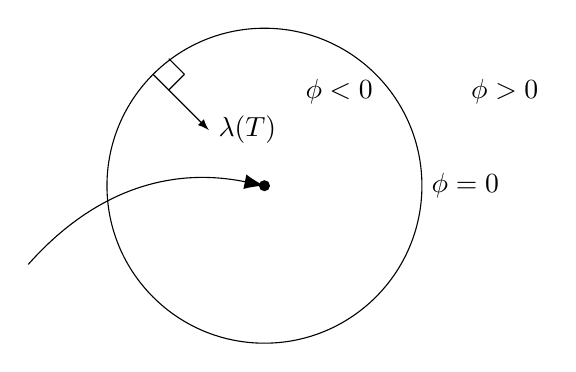
\begin{tikzpicture}
    \node [dot] at (0,0) {};
    \draw [-{Latex[scale=1.5]}] (-3,-1) to [bend left] (0,0);

    \draw (0,0) circle (2);
    \node [right] at (2,0) {$\phi=0$};
    \node [right] at (2.5,1.2) {$\phi>0$};
    \node [left] at (1.5,1.2) {$\phi<0$};

    \path (2,0) arc (0:135:2) coordinate (a);
    \draw [->] (a) -- ++(-45:1) coordinate (b);
    \node [right] at (b) {$\lambda(T)$};
    \draw ($(a)!8pt!(b)$) coordinate (c) -- ($(c)!1!-90:(a)$) coordinate (d);
    \draw (d) -- ($(d)!1!-90:(c)$);
  \end{tikzpicture}
\end{center}

Repeat process: $\tilde J = \int(H-\lambda\trans\dot x)\dif t + \Psi + \nu\trans\phi$. The optimality conditions are
\[
  \begin{dcases}
    \pder{H}{u} = 0 \\
    \dot\lambda = -\pder{H\trans}{x} \\
    \lambda(T) = \pder{\Psi\trans}{x}(x(T)) + \nu\trans\pder{\phi\trans}{x}(x(T)) \\
    \nu \ge 0 \\
    \phi(x(T)) \le 0 \\
    \nu\trans \phi(x(T)) = 0 \quad (\text{KKT})
  \end{dcases}
\]

\subsection{Initial manifold}
\begin{align}
  & \min_{x_0,u} \int L + \Psi(x(T)) + \Theta(x(0)) \\
  & \text{s.t. } \begin{aligned}[t]
    & \dot x = f(x,u) \\
    & \phi(x(T)) = 0 \\
    & \xi(x(0)) = 0
  \end{aligned}
\end{align}

\begin{align}
  \tilde J &= \int (H-\lambda\trans\dot x)\dif t + \Psi(x(T)) + \Theta(x(0)) + \nu\trans_\phi \phi(x(T)) + \nu\trans_\xi \xi(x(0)) \\
  \delta \tilde J &= \int \left[ \left( \pder{H}{x} + \dot\lambda\trans \right) \eta + \pder{H}{u}v\right] \dif t + \left[ \pder{\Psi}{x}(x(T)) + \nu\trans_\phi \pder{\phi}{x}(x(T)) - \lambda\trans(T) \right] \eta(T) \\
           & \qquad + \left[ \pder{\Theta}{x}(x(0)) + \nu\trans_\xi \pder{\xi}{x}(x(0)) + \lambda\trans(0) \right] \eta(0)
\end{align}
The optimality conditions are
\[
  \begin{dcases}
    \pder{H}{u} = 0 \\
    \dot\lambda = -\pder{H\trans}{x} \\
    \lambda(T) = -\pder{\Psi\trans}{x}(x(T)) - \nu\trans_\phi \pder{\phi\trans}{x}(x(T)) \\
    \lambda(0) = -\pder{\Theta\trans}{x}(x(0)) - \nu\trans_\xi \pder{\xi\trans}{x}(x(0))
  \end{dcases}
\]

\end{document}

\chapter{Calculus of Variations}

\section{Directional Derivatives}
\paragraph{Recall:} To minimize $g(u)$, let $u^*$ be a candidate minimizer and pitch a perturbation on $u^*$ of $\varepsilon v$, where $\varepsilon$ is the scale and $v$ is the direction. Taking Taylor's expansion at the perturbation produces

\begin{center}
  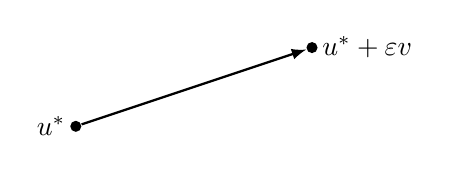
\begin{tikzpicture}
    \node [dot] (a) at (0,0) {};
    \node [dot] (b) at (3,1) {};
    \draw [>=latex,->,thick] (a) node [anchor=east] {$u^*$} -- (b) node [anchor=west] {$u^*+\varepsilon v$};
  \end{tikzpicture}
\end{center}

\begin{gather}
  g(u^* + \varepsilon v) = g(u^*) + \varepsilon \pder{g}{u}(u^*) v + o(\varepsilon) \\
  \text{FONC: } \pder{g}{u}(u^*) = 0 \hspace{3cm} 
\end{gather}

\subparagraph{Note:} $\pder{g}{u}(u^*) v$ tells us how much $g(u)$ increases/decreases in the direction of $v$.

\begin{defi}
  The directional (Gateaux) derivative is given by
  \[ \delta g(u;v) = \lim_{\varepsilon\to0} \frac{g(u+\varepsilon v)-g(u)}{\varepsilon} \]
\end{defi}

\paragraph{Example}
\[ g(u) = \frac12 u_1^2 - u_1 + 2u_2, \quad g:\R^2\to\R \]
Let's consider $e_1=[1\ 0]\trans$, $e_2=[0\ 1]\trans$. What is $\delta g(u;e_i)$, $i=1,2$?
\begin{align}
  \delta g(u;v) &= \lim_{\varepsilon\to0} \frac{g(u+\varepsilon v)-g(u)}{\varepsilon} \\
                &= \lim_{\varepsilon\to0} \frac{g(u)+\varepsilon\pder{g}{u}(u) v + o(\varepsilon) - g(u)}{\varepsilon} \\
                &= \pder{g}{u} (u) v
\end{align}
\begin{align}
  \pder{g}{u}(u) &= [u_1-1\ 2] \\
  \delta g(u;e_1) &= [u_1-1\ 2] e_1 = u_1-1 \\
  \delta g(u;e_2) &= [u_1-1\ 2] e_2 = 2 \\
\end{align}

But the beauty of directional derivatives is that they generalize beyond vectors, $u\in\R^m$, to function spaces ($\mathcal U$) or other ``objects'' like matrices.

\paragraph{Example} $M\in\R^{n\times n}$, $F(M)=M^2$

What is $\pder{F}{M}$? (ponder at home\dots)

We can easily compute $\delta F(M;N)$!
\begin{align}
  F(M+\varepsilon N) &= (M+\varepsilon N)(M+\varepsilon N) = M^2 + \varepsilon M N + \varepsilon N M + \varepsilon^2 N^2 \\
  \delta F(M;N) &= \lim_{\varepsilon\to0} \frac{F(M+\varepsilon N)-F(M)}{\varepsilon} \\
                     &= \lim_{\varepsilon\to0} \frac{\varepsilon M N + \varepsilon N M + \varepsilon^2 N^2}{\varepsilon} = MN + NM
\end{align}

\paragraph{Infinite Dimensional Optimization}
Let $u\in\mathcal U$ (function space) and let $J(u)$ be the cost:
\[ \min_{u\in\mathcal U} J(u) \]

\begin{thm}
  If $u^*\in\mathcal U$ is a (local) minimizer then
  \[ \delta J(u^*;v) = 0, \quad \forall v\in\mathcal U \]
\end{thm}

\paragraph{Example} Find minimizer $u^*$ to
\[ J(u) = \int_0^T L(u(t)) \dif t \]
\begin{align}
  J(u+\varepsilon v) - J(u) &= \int_0^T L(u(t)+\varepsilon v(t)) \dif t - \int_0^T L(u(t)) \dif t, \quad u,v\in\mathcal U \\
                            &= \int_0^T \left[ L(u(t)) + \varepsilon \pder{L}{u}(u(t)) v(t) + o(\varepsilon) - L(u(t)) \right] \dif t \\
  \delta J(u^*;v) &= \lim_{\varepsilon\to0} \frac{J(u+\varepsilon v)-J(u)}{\varepsilon} \\
                            &= \lim_{\varepsilon\to0} \frac{\int_0^T \varepsilon \pder{L}{u}(u(t)) v(t) \dif t + o(\varepsilon)}{\varepsilon} \\
                            &= \int_0^T \pder{L}{u}(u(t)) v(t) \dif t \\
\end{align}
$u^*$ optimizer:
\begin{gather}
  \delta J(u^*;v) = \int_0^T \pder{L}{u}(u(t)) v(t) \dif t = 0 \quad \forall v\in\mathcal U \\
  \Updownarrow \\
  \pder{L}{u} (u(t)) = 0 \quad \forall t\in[0,T]
\end{gather}
But, we want \emph{optimal control}! We want our cost to look like
\begin{gather}
  \int_0^T L(x(t),u(t)) \dif t \\
  \dot x = f(x,u)
\end{gather}

\section{Calculus of Variations}
What happens to $x(t)$ when $u(t)$ changes to $u(t)+\varepsilon v(t)$? Let the system be given by
\[ \begin{cases}
    \dot x = f(x,u) \\
    x(0) = x_0
  \end{cases} \]
After perturbation of $u$, the new system is
\[ \begin{cases}
    \dot{\hat x} = f(\hat x,u+\varepsilon v) \\
    x(0) = x_0
  \end{cases} \]

\pgfmathsetseed{11}
\begin{figure}
  \centering
  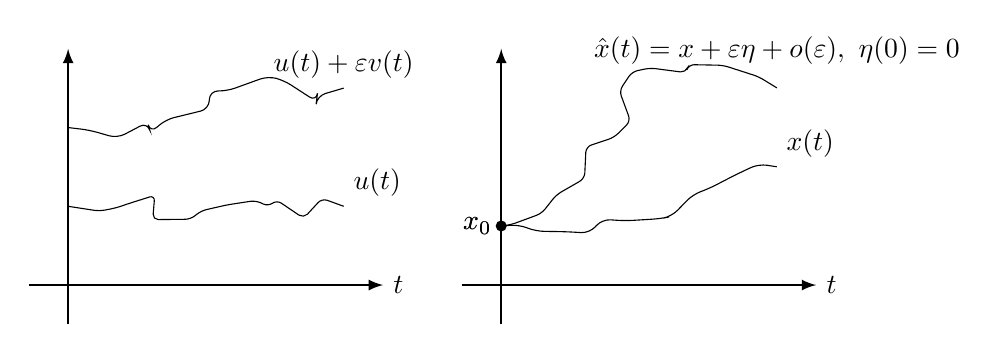
\begin{tikzpicture}
    \draw [thick,->] (-0.5,0) -- (4,0) node [anchor=west] {$t$};
    \draw [thick,->] (0,-0.5) -- (0,3) node [anchor=east] {};
    \draw [decorate, decoration={random steps, segment length=7pt, amplitude=5pt}, rounded corners=2pt] (0,1) to[in=180,out=0,distance=3.5cm] (3.5,1) node [anchor=south west] {$u(t)$};
    \draw [decorate, decoration={random steps, segment length=8pt, amplitude=5pt}, rounded corners=3pt] (0,2) to[in=180,out=0,distance=3cm] (3.5,2.5) node [anchor=south] {$u(t)+\varepsilon v(t)$};

    \draw [thick,->] (5,0) -- (9.5,0) node [anchor=west] {$t$};
    \draw [thick,->] (5.5,-0.5) -- (5.5,3) node [anchor=east] {};
    \draw [decorate, decoration={random steps, segment length=8pt, amplitude=4pt}, rounded corners=3pt] (5.5,0.75) node [anchor=east] {$x_0$} to[in=200,out=0,distance=3cm] (9,1.5) node [anchor=south west] {$x(t)$};
    \draw [decorate, decoration={random steps, segment length=8pt, amplitude=5pt}, rounded corners=2pt] (5.5,0.75) node [anchor=east] {$x_0$} to[in=170,out=30,distance=3cm] (9,2.5) node [anchor=south,yshift=5pt] {$\hat x(t)=x+\varepsilon\eta+o(\varepsilon),\ \eta(0)=0$};
    \node [dot] at (5.5,0.75) {};
  \end{tikzpicture}
  \caption{Variation in $u$ causes a variation in $x$.}
  \label{fig:var_u_x}
\end{figure}

\noindent
Consider
\[ \tilde x=x+\varepsilon \eta, \]
where
\begin{alignat}{2}
  \dot x&=f(x,u), & x(0) &= x_0 \\
  \dot \eta &= \pder{f}{x}(x,u) \eta + \pder{f}{u}(x,u) v, \qquad & \eta(0) &= 0
\end{alignat}

\begin{thm}
  If $f$ is continuously differentiable in $x$ and $u$ then
  \[ \hat x(t) = \tilde x(t) + o(\varepsilon) \]
  \begin{proof}
    \mbox{}
    \begin{enumerate}[label=\roman*)]
    \item Initial conditions:
      \begin{align}
        \hat x(0) &= x_0 \\
        \tilde x(0) &= x(0) + \varepsilon \eta(0) = x_0
      \end{align}
    \item Dynamics:
      \begin{align}
        \dot{\hat x} &= f(\hat x,u+\varepsilon v) \\
        \dot{\tilde x} &= \dot x + \varepsilon \dot \eta = f(x,u) + \varepsilon \pder{f}{x}(x,u)\eta + \varepsilon \pder{f}{u}(x,u) v \\
                     &= f(x+\varepsilon\eta,u+\varepsilon v) + o(\varepsilon) \\
                     &= f(\tilde x,u+\varepsilon v) + o(\varepsilon)
      \end{align}
      We can see that the dynamics of $\hat x(t)$ are equal to those of $\tilde x(t)$ plus higher order terms:
      \begin{align}
        \dot{\tilde x} &= f(\tilde x,u+\varepsilon v) + o(\varepsilon) \\
        \dot{\hat x} &= f(\hat x,u+\varepsilon v)
      \end{align}
      Therefore, if our perturbation is small enough, we can model $\hat x(t)$ as $\tilde x(t)$.
    \end{enumerate}
  \end{proof}
\end{thm}

\begin{framed}
  \hypertarget{taylor_2var}{}
  Note: Taylor expansion with two elements is
  \begin{align}
    h(w+\varepsilon v,z+\varepsilon y) &= h(w,z+\varepsilon y) + \pder{h}{w}(w,z+\varepsilon y)\varepsilon v + o(\varepsilon) \\
                                       &= \left\{ h(w,z) + \pder{h}{z}(w,z)\varepsilon y + o(\varepsilon) \right\} \\
                                       & \qquad + \left\{ \pder{h}{w}(w,z)\varepsilon v + \underbrace{\pder{^2 h}{z\partial w}\varepsilon v \odot \varepsilon y}_{o(\varepsilon)} + o(\varepsilon) \right\} \\
                                       &= h(w,z) + \pder{h}{z}\varepsilon y + \pder{h}{w}\varepsilon v + o(\varepsilon)
  \end{align}
\end{framed}

% 2017/01/26
\paragraph{Last class:} \mbox{}
\begin{enumerate}
\item $u\in\U$ (space of functions), $J:\U\to\R$ (cost).

  FONC: If $u^*$ is optimal, then
  \[ \delta J(u;\nu) = 0 \quad \forall \nu\in\U, \]
  where the directional derivative is given by
  \[ \delta J(u;\nu) = \lim_{\varepsilon\to0} \frac{J(u+\varepsilon \nu)-J(u)}{\varepsilon}. \]
\item If
  \[ \begin{cases}
      \dot x = f(x,u) \\
      x(0) = x_0
    \end{cases} \]
  then a variation in $u$:
  \[ u \longmapsto u+\varepsilon \nu \]
  results in a variation in $x$:
  \[ x \longmapsto x+\varepsilon\eta + o(\varepsilon) \]
  See \autoref{fig:var_u_x}. Note $\eta(0)=0$.
\end{enumerate}

\subsection{An (Almost) Optimal Control Problem}

Let $\dot x=f(x)$, $x(0)=x_0$. Note we get to pick the initial condition!
\subparagraph{Problem}
\begin{gather}
  \min_{x_0\in\R^m} J(x_0) = \int_0^T L(x(t)) \dif t \\
  \text{s.t. } \begin{cases}
    \dot x(t) = f(x(t)) & \text{the \emph{constraint}! (equality)} \\
    x(0)=x_0
  \end{cases}
\end{gather}
Note every constraint needs a Lagrange multiplier. We have infinitely many constraints:
\[ \dot x(t) = f(x(t)) \quad \forall t\in[0,T] \]
We need $\lambda(t)$ as a function of $t$. Also, the sum in the Lagrangian has to become an integral. The continuous-time Lagrangian thus becomes
\[ \tilde J(x_0,\lambda) = \int_0^T \Big[ L(x(t)) + \lambda\trans(t) (f(x(t))-\dot x(t)) \Big] \dif t \]
The task is to perturb $x_0$ as $x_0\longmapsto x_0+\varepsilon \nu$, $\nu\in\R^m$ and compute
\[ \delta \tilde J(x_0;\nu) = \lim_{\varepsilon\to0} \frac{\tilde J(x_0+\varepsilon \nu)-\tilde J(x_0)}{\varepsilon} \]
and make this equal to 0 $\forall \nu\in\R^m$. The variation in $x$ is

\pgfmathsetseed{11}
\begin{center}
  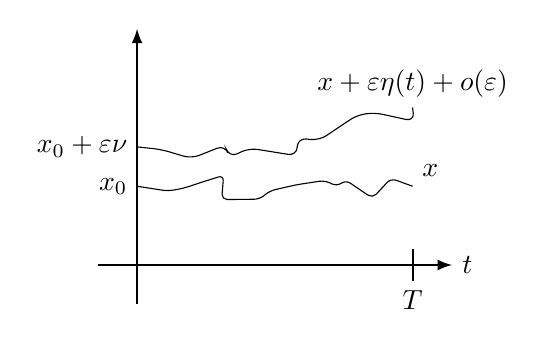
\begin{tikzpicture}
    \draw [->,thick] (-0.5,0) -- (4,0) node [anchor=west] {$t$};
    \draw [->,thick] (0,-0.5) -- (0,3);
    \draw [decorate, decoration={random steps, segment length=7pt, amplitude=5pt}, rounded corners=2pt] (0,1) node [anchor=east] {$x_0$} to[in=180,out=0,distance=3.5cm] (3.5,1) node [anchor=south west] {$x$};
    \draw [decorate, decoration={random steps, segment length=9pt, amplitude=5pt}, rounded corners=3pt] (0,1.5) node [anchor=east] {$x_0+\varepsilon \nu$} to[in=200,out=0,distance=3.5cm] (3.5,2) node [anchor=south] {$x+\varepsilon\eta(t)+o(\varepsilon)$};
    \draw [thick] (3.5,0.2) -- (3.5,-0.2) node [anchor=north] {$T$};
  \end{tikzpicture}
\end{center}

Note:

\hspace{\parindent}
\begin{tabular}{cl}
  $x_0$ & decision variable \\
  $\nu$ & variation in $x_0$ \\
  $x(t)$ & trajectory starting at $x_0$ \\
  $\eta(t)$ & change in trajectory resulting from $\nu$-variation in $x_0$ \\
  $\lambda(t)$ & time-varying Lagrange multiplier
\end{tabular}

\begin{align}
  \tilde J(x_0+\varepsilon \nu) &= \int_0^T \Big\{ L(x(t)) + \lambda\trans(t) [f(x(t)+\varepsilon\eta(t)) - \dot x(t) - \varepsilon\dot\eta(t)] \Big\} \dif t + o(\varepsilon) \\
                                &= \int_0^T \left[ L(x) + \varepsilon\pder{L}{x}(x)\eta + \lambda\trans \left( f(x) + \varepsilon\pder{f}{x}(x)\eta - \dot x - \varepsilon\dot\eta \right) \right] \dif t + o(\varepsilon) \\
  \tilde J(x_0+\varepsilon \nu) - \tilde J(x_0) &= \int_0^T \left[ \varepsilon\pder{L}{x}(x)\eta + \lambda\trans\left( \varepsilon\pder{f}{x}\eta - \varepsilon\dot\eta \right) \right] \dif t + o(\varepsilon) \\
  \delta \tilde J (x_0;\nu) &= \int_0^T \left[ \pder{L}{x}(x)\eta + \lambda\trans\left( \pder{f}{x}\eta - \dot\eta \right) \right] \dif t
\end{align}
A powerful idea: we want $\delta\tilde J(x_0;\nu)=0$ $\forall \nu$. Somehow get this in the form
\[ \int_0^T \Big(\text{stuff}(t)\Big) \eta(t) \dif t = 0 \]
We can pick $\text{stuff}(t)=0$ $\forall t\in[0,T]$.

In $\delta\tilde J(x_0;\nu)$ we have $\dot\eta$ (problem!). We can solve this using \emph{integration by parts}.
\[ \int_0^T \lambda\trans \dot\eta \dif t = \lambda\trans(T)\eta(T) - \lambda\trans(0)\eta(0) - \int_0^T \dot\lambda\trans\eta \dif t \]
Hence,
\[
  \delta\tilde J(x_0;\nu) = \int_0^T \underbrace{\big( \pder{L}{x} + \lambda\trans\pder{f}{x} + \dot\lambda\trans \big)}_{\text{pick}=0} \eta \dif t - \underbrace{\lambda\trans(T)}_{\text{pick}=0} \eta(T) + \lambda\trans(0) \underbrace{\eta(0)}_{\nu}
\]
We are free to pick $\lambda$ freely if it gives $\delta\tilde J=0$.
\[ \text{Pick: } \begin{cases}
    \dot\lambda(t) = -\pder{L\trans}{x}(x(t)) - \pder{f\trans}{x}(x(t)) \lambda(t) \\
    \lambda(T) = 0 & \text{backwards diff. eq}
  \end{cases} \]
Under this choice of $\lambda$ we get
\[ \delta\tilde J(x_0;\nu) = \lambda\trans(0) \nu \]
This is linear in $\nu$ so the FONC is $\lambda(0)=0$.

Moreover, we really have a ``normal'' optimization problem
\begin{gather}
  \min_{x_0\in\R^m} \tilde J(x_0) \\
  \delta \tilde J(x_0;\nu) = \pder{\tilde J}{x_0} (x_0) \nu
\end{gather}
which means that
\[ \pder{\tilde J}{x_0} = \lambda\trans(0) \]
If $x_0^*$ minimizes
\begin{gather}
  \int_0^T L(x(t)) \dif t \\
  \text{s.t. } \begin{cases}
    \dot x(t) = f(x(t)) \\
    x(0) = x_0^*
  \end{cases}
\end{gather}
then
\[ \lambda(0) = \bm 0 \]
where $\lambda(t)$ satisfies
\[ \begin{cases}
    \dot \lambda(t) = -\pder{L\trans}{x}(x(t)) - \pder{f\trans}{x}(x(t)) \lambda(t) \\
    \lambda(T) = 0
  \end{cases} \]

\paragraph{So what?} We actually have a two-point boundary value problem. 
\begin{align}
  \dot x &= f(x) & \dot\lambda &= -\pder{L\trans}{x} - \pder{f\trans}{x} \lambda \\
  x(0) &= x_0 & \lambda(T) &= 0
\end{align}

\begin{center}
  \begin{tikzpicture}
    \draw [thick,->] (0,0) -- (4,0) node [anchor=west] {$t$};
    \draw [thick,->] (0,0) -- (0,3);
    \draw (-0.2,1.5) node [anchor=east] {$x_0$} -- (0.2,1.5);
    \draw [->,>={Straight Barb[scale length=2]}] (0,1.5) parabola bend (0.6,2) (1.5,1.5);
    \draw (1.5,1.5) parabola bend (2,1.3) (3.5,2.5);

    \draw [thick,->] (6,0) -- (10,0) node [anchor=west] {$t$};
    \draw [thick,->] (6,0) -- (6,3);
    \draw (9.5,0.2) -- (9.5,-0.2) node [anchor=north] {$T$};
    \draw [-{Straight Barb[scale length=2]}] (9.5,0) .. controls (8.25,0) and (9,1.5) .. (8,1.5) node [anchor=south] {$\lambda$};
    \draw (8,1.5) .. controls (7,1.25) .. (6,1.5);
    \draw (6.2,1.5) -- (5.8,1.5) node [anchor=east] {$\lambda(0)$};
  \end{tikzpicture}
\end{center}
We want to find $x_0$ that gives $f(x)$ such that after solving backwards for $\lambda(t)$, we find that
\[ \lambda(0) = \pder{\tilde J\trans}{x_0} = 0. \]
This leads to the following:

\paragraph{An algorithm} \mbox{}

\begin{algorithm}
  \begin{algorithmic}
    \State Pick $x_{0,0}$
    \State $k=1$
    \Repeat
    \State Simulate $x(t)$ from $x_{0,k}$ over $[0,T]$
    \State Simulate $\lambda(t)$ from $\lambda(T)=0$ backwards using $x(t)$
    \State Update $x_{0,k}$ as
    $ x_{0,k+1} = x_{0,k} - \gamma\lambda(0) $ \Comment{$\lambda(0)$ is the gradient}
    \State $k\coloneqq k+1$
    \Until $\lambda(0)=0$
  \end{algorithmic}
\end{algorithm}

\paragraph{Example:} \texttt{optinit.m}

\[ \dot x = Ax, \quad L=x\trans Qx-q, \quad Q=Q\trans \succ 0 \]
\vspace{-2em}
\begin{align}
  \dot \lambda &= -2Qx - A\trans\lambda \\
  \lambda(0) &= 0
\end{align}

% 2017/01/31
\subsection{Optimal Timing Control}
When to switch between modes?
\begin{equation}
  \begin{aligned}
    \dot x &= \begin{cases}
      f_1(x) & \text{if } t\in[0,\tau) \\
      f_2(x) & \text{if } t\in[\tau,T]
    \end{cases} \\
    x(0) &= x_0
  \end{aligned} \label{eq:otc}
\end{equation}

\begin{center}
  \begin{tikzpicture}
    \draw [->,thick] (-0.2,0) -- (5.5,0) node [anchor=west] {$t$};
    \draw [->,thick] (0,-0.2) -- (0,3.2);
    \draw (4.8,0.2) -- (4.8,-0.2) node [anchor=north] {$T$};
    \draw (2.2,0.2) -- (2.2,-0.2) node [anchor=north] {$\tau$};
    \draw (0.2,1) -- (-0.2,1) node [anchor=east] {$x_0$};
    \draw (0,1) parabola (2.2,2.8);
    \draw (2.2,2.8) parabola [bend at end] (4.8,1.2) node [anchor=west] {$x$};
    \node at (1,1.8) {$f_1$};
    \node at (4,1.8) {$f_2$};
  \end{tikzpicture}
\end{center}

\begin{align}
  & \min_\tau \int_0^T L(x(t)) \dif t = J(\tau) \\
  & \text{s.t.~\eqref{eq:otc} holds}
\end{align}

\begin{enumerate}[label=Step \arabic*:]
\item Augment cost with constraint
  \[ \tilde J = \int_0^\tau \Big[ L(x) + \lambda\trans(f_1(x)-\dot x) \Big] \dif t + \int_\tau^T \Big[ L(x) + \lambda\trans(f_2(x)-\dot x) \Big] \dif t \]
\item Variation $\tau\longmapsto\tau+\varepsilon\theta$
  \begin{center}
    \begin{tikzpicture}
      \draw [->,thick] (-0.2,0) -- (5.5,0) node [anchor=west] {$t$};
      \draw [->,thick] (0,-0.2) -- (0,3.2);
      \draw (4.8,0.2) -- (4.8,-0.2) node [anchor=north] {$T$};
      \draw (2.2,0.2) -- (2.2,-0.2) node [anchor=north] {$\tau$};
      \draw (3,0.2) -- (3,-0.2) node [anchor=north,yshift=3pt] {$\tau+\varepsilon\theta$};
      \draw (0.2,1) -- (-0.2,1) node [anchor=east] {$x_0$};
      \draw (0,1) parabola (2.2,1.8);
      \draw (2.2,1.8) parabola [bend at end] (4.8,1.2) node [anchor=west] {$x$};
      \node at (1,1.8) {$f_1$};
      \node at (3.6,1.7) {$f_2$};

      \begin{scope}
        \clip (4.8,4) rectangle (2.2,1.8);
        \draw [dashed] (2.2,1.8) parabola bend (0,1) (3,2.5);
        \draw [dashed] (3,2.5) parabola [bend at end] (5.4,1.9);
      \end{scope}
      \node [anchor=west] at (4.8,1.9) {$x+\varepsilon\eta+o(\varepsilon)$};
      \node at (2.4,2.4) {$f_1$};
      \node at (3.9,2.5) {$f_2$};
    \end{tikzpicture}
  \end{center}
\item Compute $\delta\tilde J(\tau;\theta)$
\end{enumerate}
\begin{align}
  \tilde J(\tau+\varepsilon\theta) &= \int_0^{\tau+\varepsilon\theta} \Big\{ L(x+\varepsilon\eta) + \lambda\trans[f_1(x+\varepsilon\eta)-\dot x-\varepsilon\dot\eta] \Big\} \dif t \\
                                   & \qquad + \int_{\tau+\varepsilon\theta}^T \Big\{ L(x+\varepsilon\eta) + \lambda\trans[f_2(x+\varepsilon\eta)-\dot x-\varepsilon\dot\eta] \Big\} \dif t + o(\varepsilon) \\
  \intertext{Note that $\eta=\dot\eta=0$ on $[0,\tau)$.}
  \tilde J(\tau+\varepsilon\theta) &= \int_0^\tau \Big\{ L(x) + \lambda\trans[f_1(x)-\dot x] \Big\} \dif t \\
                                   & \qquad + \int_\tau^{\tau+\varepsilon\theta} \Big\{ \underbrace{L(x+\varepsilon\eta)}_{L(x)+\varepsilon\pder{L}{x}\eta} + \lambda\trans[\underbrace{f_1(x+\varepsilon\eta)}_{f_1(x)+\varepsilon\pder{f_1}{x}\eta} - \dot x-\varepsilon\dot\eta] \Big\} \dif t \\
                                   & \qquad + \int_{\tau+\varepsilon\theta}^T \Big\{ \underbrace{L(x+\varepsilon\eta)}_{L(x)+\varepsilon\pder{L}{x}\eta} + \lambda\trans[\underbrace{f_2(x+\varepsilon\eta)}_{f_2(x)+\varepsilon\pder{f_2}{x}\eta} - \dot x-\varepsilon\dot\eta] \Big\} \dif t + o(\varepsilon) \displaybreak \\
  \delta\tilde J(\tau;\theta) &= \lim_{\varepsilon\to0} \frac{\tilde J(\tau+\varepsilon\theta) - \tilde J(\tau)}{\varepsilon} \\
  \tilde J(\tau+\varepsilon\theta) - \tilde J(\tau) &= \int_0^\tau 0\cdot\dif t + \underbrace{ \int_\tau^{\tau+\varepsilon\theta} \left[ \varepsilon\pder{L}{x}\eta + \lambda\trans \Big(f_1(x)+\varepsilon\pder{f_1}{x}\eta - f_2(x) - \varepsilon\dot\eta \Big) \right] \dif t }_{\displaystyle I_1} \\
                                   & \qquad + \underbrace{ \int_{\tau+\varepsilon\theta}^T \left[ \varepsilon\pder{L}{x}\eta + \lambda\trans \Big( \varepsilon\pder{f_2}{x}\eta - \varepsilon\dot\eta \Big) \right] \dif t }_{\displaystyle I_2} + o(\varepsilon)
\end{align}

\begin{framed}
  \begin{thm}[Mean-value theorem]
    \[ \int_{t_1}^{t_2} h(t) \dif t = (t_2-t_1) h(\xi) \quad \text{for some}\ \xi\in[t_1,t_2] \]
  \end{thm}
\end{framed}

\noindent
The first integral is
\begin{align}
  I_1 &= \int_\tau^{\tau+\varepsilon\theta} \left\{ \varepsilon\pder{L}{x}\eta + \lambda\trans \left[f_1(x)+\varepsilon\pder{f_1}{x}\eta-\varepsilon\dot\eta-f_2(x)\right] \right\} \dif t \\
      &= \varepsilon\theta \Big\{ \lambda\trans(\xi) \big[ f_1(x(\xi)) - f_2(x(\xi)) \big] \Big\} + o(\varepsilon)
\end{align}
Note that as $\varepsilon\to0$, $\xi\to\tau$. Using integration by parts, the second integral is
\begin{align}
  \int_\tau^T \lambda\trans \dot\eta \dif t &= \lambda\trans(T) \eta(T) - \lambda\trans(\tau) \underbrace{\eta(\tau)}_{=0} - \int_\tau^T \dot\lambda\trans \eta \dif t \\
  I_2 &= \int_\tau^T \left[ \varepsilon\pder{L}{x}\eta + \lambda\trans \Big( \varepsilon\pder{f_2}{x}\eta - \varepsilon\dot\eta \Big) \right] \dif t - \underbrace{ \int_\tau^{\tau+\varepsilon\theta} \left[ \varepsilon\pder{L}{x}\eta + \lambda\trans \Big( \varepsilon\pder{f_2}{x}\eta - \varepsilon\dot\eta \Big) \right] \dif t }_{o(\varepsilon)} \\
                                            &= \varepsilon \int_\tau^T \left[ \pder{L}{x} + \lambda\trans \pder{f_2}{x} + \dot\lambda\trans \right] \eta \dif t - \varepsilon \lambda\trans(T)\eta(T) + o(\varepsilon)
\end{align}
Hence,
\begin{align}
  \delta\tilde J(\tau;\theta) &= \lim_{\varepsilon\to0} \frac{\tilde J(\tau+\varepsilon\theta) - \tilde J(\tau)}{\varepsilon} \\
                              &= \theta\lambda\trans(\tau) \Big[ f_1(x(\tau)) - f_2(x(\tau)) \Big] + \int_\tau^T \left[ \pder{L}{x} + \lambda\trans \pder{f_2}{x} + \dot\lambda\trans \right] \eta \dif t - \lambda\trans(T)\eta(T)
\end{align}

\begin{enumerate}[resume*]
\item Select the \emph{costate} $\lambda(t)$. The key idea is to get rid of any term that has $\eta$ in it, i.e.
  \begin{align}
    \dot\lambda &= -\pder{L\trans}{x} - \pder{f_2\trans}{x} \lambda \quad \text{on } [\tau,T] \\
    \lambda(T) &= 0
  \end{align}
\item With this choice of $\lambda(t)$, we have
  \[ \delta\tilde J(\tau;\theta) = \theta\lambda\trans(\tau) \Big[ f_1(x(\tau)) - f_2(x(\tau)) \Big] = \pder{\tilde J}{\tau} \theta. \]
  Therefore,
  \[ \pder{\tilde J}{\tau} = \lambda\trans(\tau) \Big[ f_1(x(\tau)) - f_2(x(\tau)) \Big] = 0 \quad \text{(for optimality)} \]
\end{enumerate}

\paragraph{Algorithm} \mbox{}
\begin{algorithm}
  \begin{algorithmic}
    \State Pick $\tau_0$
    \State $k=0$
    \Repeat
    \State Simulate $x$ forward in time from $x(0)=x_0$
    \State Simulate $\lambda$ backwards from $\lambda(T)=0$
    \State Update $\tau_k$ as
    $ \tau_{k+1} = \tau_k - \gamma\lambda\trans(\tau_k) \big[ f_1(x(\tau_k)) - f_2(x(\tau_k)) \big] $
    \State $k\coloneqq k+1$
    \Until $\Vert \lambda\trans(f_1-f_2) \Vert < \varepsilon$
  \end{algorithmic}
\end{algorithm}

Where are we going? Come up with general principles for $\min_{u\in\mathcal U} J(u)$:
\begin{itemize}
\item Costate equations
\item Optimality conditions
\item Algorithms
\item Applications
\end{itemize}

%%% Local Variables:
%%% mode: latex
%%% TeX-master: "../notes"
%%% End:

\chapter{The Maximum Principle}

% 2017/02/02
\section{The Bolza Problem}
Up until now, we have optimized with respect to finite-dimensional parameters. Today, we will minimize with respect to $u\in\mathcal U$.

\begin{align}
  & \min_{u\in\mathcal U} J(u) = \int_0^T L(x(t),u(t),t) \dif t + \underbrace{\Psi(x(T))}_{\substack{\text{terminal cost}\\ \text{(parking cost)}}} \\
  & \begin{aligned}
    \text{s.t.}\quad \dot x(t) &= f(x(t),u(t),t) \\
    x(0) &= x_0
  \end{aligned}
\end{align}
Assume that $f$ and $L$ are $C^1$ in $x,u$ and piecewise continuous in $t$. Then, a small change in $u$ causes small changes in $f$ and $L$. The variation: $u\longmapsto u+\varepsilon v$, $\varepsilon\in\R$, $v\in\mathcal U$. See \autoref{fig:var_u_x}.
\begin{align}
  \tilde J(u) &= \int_0^T \left[ L(x,u,t) + \lambda\trans (f(x,u,t)-\dot x) \right] \dif t + \Psi(x(T)) \\
  \tilde J(u+\varepsilon v) &= \int_0^T \left[ L(x+\varepsilon\eta,u+\varepsilon v, t) + \lambda\trans(f(x+\varepsilon\eta,u+\varepsilon v, t) - \dot x - \varepsilon\dot\eta) \right] \dif t \\
              & \qquad + \Psi(x(T)+\varepsilon\eta(T)) + o(\varepsilon) \\
  \tilde J(u+\varepsilon v) - \tilde J(u) &= \int_0^T \bigg[ L(x+\varepsilon\eta,u+\varepsilon v,t) - L(x,u,t) \\
              & \qquad\qquad + \lambda\trans\Big( f(x+\varepsilon\eta,u+\varepsilon v,t) - f(x,u,t) - \dot x - \varepsilon\dot\eta + \dot x \Big) \bigg] \dif t \\
              & \qquad + \Psi(x(T)+\varepsilon\eta(T)) - \Psi(x(T)) + o(\varepsilon) \\
              &= \int_0^T \left[ \pder{L}{x}\varepsilon\eta + \pder{L}{u}\varepsilon v + \lambda\trans\bigg( \pder{f}{x}\varepsilon\eta + \pder{f}{u}\varepsilon v - \varepsilon\dot\eta \bigg) \right] \dif t \\
              & \qquad + \pder{\Psi}{x}(x(T))\varepsilon\eta(T) + o(\varepsilon) \\
  \shortintertext{(See \hyperlink{taylor_2var}{Taylor expansion with respect to two variables}.)}
  \delta\tilde J(u;v) &= \int_0^T \left(\pder{L}{u} + \lambda\trans\pder{f}{u}\right)v\dif t + \int_0^T \left[\left(\pder{L}{x} + \lambda\trans\pder{f}{x}\right)\eta - \lambda\trans\dot\eta\right] \dif t \\
              & \qquad + \pder{\Psi}{x}(x(T))\eta(T) \\
  \shortintertext{Integrating by parts,}
  \int_0^T \lambda\trans\dot\eta\dif t &= \lambda\trans(T)\eta(T) - \lambda\trans(0)\eta(0) - \int_0^T \dot\lambda\trans\eta \dif t \\
              &= \lambda\trans(T)\eta(T) - \int_0^T \dot\lambda\trans\eta \dif t \\
  \delta\tilde J(u;v) &= \int_0^T \left(\pder{L}{u}+\lambda\trans\pder{f}{u}\right) v\dif t + \int_0^T \left(\pder{L}{x}+\lambda\trans\pder{f}{x} + \dot\lambda\trans\right)\eta \dif t \\
              & \qquad + \left(\pder{\Psi}{x}(x(T))-\lambda\trans(T)\right)\eta(T) \\
  \intertext{For optimality, we need the directional derivative to be zero for every $v\in\mathcal U$, where $v$ represents the direction of the derivative. Therefore, the term $(\pder{L}{u}+\lambda\trans\pder{f}{u})$ in the first integral has to be identically zero. Thus, we need}
              & \begin{dcases}
                \pder{L}{u} + \lambda\trans\pder{f}{u} = 0, & \forall t\in[0,T] \\
                \pder{L}{x} + \lambda\trans\pder{f}{x} + \dot\lambda\trans = 0, & \forall t\in[0,T] \\
                \pder{\Psi}{x}(x(T)) - \lambda\trans(T) = 0
              \end{dcases}
\end{align}
\begin{framed}
  \begin{defi}
    Let the \emph{Hamiltonian} $H(x,u,t,\lambda)$ be given by
    \[ H(x,u,t,\lambda) = L(x,u,t) + \lambda\trans f(x,u,t) \]
  \end{defi}
\end{framed}
\begin{thm}
  For $u$ to solve the Bolza problem, it has to satisfy
  \[ \pder{H}{u}(x,u,t,\lambda) = 0, \]
  where the \emph{costate} satisfies
  \[ \begin{dcases}
      \dot\lambda = - \pder{H\trans}{x}(x,u,t,\lambda) \\
      \lambda(T) = \pder{\Psi\trans}{x}(x(T))
    \end{dcases} \]
\end{thm}

\paragraph{Example} \mbox{}
\begin{align}
  & \min_u \int_0^1 \frac12 u^2(t) \dif t + \frac12 x^2(1) \\
  & \text{s.t. } \begin{cases}
    \dot x = u, & x,u\in\R \\
    x(0) = 1
  \end{cases}
\end{align}
\begin{align}
  H &= \frac12 u^2 + \lambda u \\
  \pder{H}{u} &= u + \lambda = 0 \Longrightarrow u=-\lambda \\
  \dot\lambda &= -\pder{H}{x} = 0 \Longrightarrow \lambda(t) = c \\
  \lambda(T) &= c = \pder{\Psi}{x}(x(1)) = x(1) \\
  \dot x &= u = -c \Longrightarrow x(t) = -ct + x(0) = -ct + 1 \\
  x(1) &= -c + 1 \\
  \lambda(1) &= c = x(1) = -c + 1 \Longrightarrow c = \frac12 \\
  \Aboxed{u^* &= -\frac12}
\end{align}
\begin{center}
  \begin{tikzpicture}
    \draw [thick,->] (-0.5,0) -- (4,0) node [anchor=west] {$t$};
    \draw [thick,->] (-0.5,5) -- (4,5) node [anchor=west] {$t$};
    \draw [thick,->] (0,3.5) -- (0,6) node [anchor=south] {$u$};
    \draw [thick,->] (0,-1) -- (0,2.5) node [anchor=south] {$x$};

    \draw (-0.2,4) node [anchor=east] {$-\dfrac12$} -- (3.5,4);
    \draw (3.5,4.8) -- (3.5,5.2) node [anchor=south] {$1$};

    \draw (-0.2,2) node [anchor=east] {$1$} -- (0.2,2);
    \draw (-0.2,1) node [anchor=east] {$\dfrac12$} -- (0.2,1);
    \draw (3.5,-0.2) node [anchor=north] {$1$} -- (3.5,0.2);
    \draw (0,2) -- (3.5,1);
  \end{tikzpicture}
\end{center}

We really used five different equations to solve this!
\begin{enumerate}[label=\roman*)]
\item $\displaystyle \pder{H}{u} = 0$
\item $\displaystyle \dot\lambda = - \pder{H\trans}{x}$
\item $\displaystyle \lambda(T) = \pder{\Psi\trans}{x}(x(T))$
\item $\dot x = f(x,u,t)$
\item $x(0) = x_0$
\end{enumerate}
There is a sixth condition that is pretty useful if $L$ and $f$ do not depend on $t$ ($L(x,u)$, $f(x,u)$). This is called a \emph{conservative system}. Then, along optimal trajectories (equations i-v are satisfied), the total time derivative of the Hamiltonian is
\[
  \frac{\dif}{\dif t} H = \underbrace{\pder{H}{t}}_{\mathclap{\substack{0\\ H(x,u,\lambda)}}} + \underbrace{\pder{H}{x}}_{-\dot\lambda\trans} \dot x + \underbrace{\pder{H}{u}}_{\mathclap{\substack{0\\ \text{ $u$ is optimal}}}} \dot u + \underbrace{\pder{H}{\lambda}}_{\mathclap{f\trans=\dot x\trans}} \dot\lambda
  = -\dot\lambda\trans \dot x + \dot x\trans \dot\lambda = 0
\]
Therefore, for conservative systems,
\begin{enumerate}[resume*]
\item $H$ is constant along optimal trajectories. (Hamilton's Principle in analytical mechanics)
\end{enumerate}
Back to the example,
\[ H = \frac12 u^2 + \lambda u = \frac12 c^2 - c^2 = -\frac12 c^2 = -\frac18 \]

% 2017/02/07
The Hamiltonian
\[ H(x,u,t,\lambda) = L(x,u,t) + \lambda\trans f(x,u,t) \]
lets us write the Lagrangian as
\[ \tilde J(u) = \int_0^T \big[ L + \lambda\trans(f-\dot x) \big] \dif t + \Psi = \int_0^T \big(H - \lambda\trans \dot x \big) \dif t + \Psi \]
The optimality conditions are
\begin{gather}
  \pder{H}{u} = 0,
  \label{eq:Hoptcond}
\end{gather}
where
\begin{gather}
  \begin{dcases}
    \dot\lambda = -\pder{H\trans}{x} \\
    \lambda(T) = \pder{\Psi}{x}(x(T))
  \end{dcases}
  \label{eq:Hoptcond2}
\end{gather}

\paragraph{Example} Hamilton's Principle

Let $q$ be the generalized coordinates (positions and angles). Then, $\dot q = u$ are generalized velocities, which we assume we can control. Let $T(q,u)=u\trans M(q) u$, $M\succ0$, be the kinetic energy and $V(q)$ be the potential energy.

For conservative systems, the following quantity is minimized:
\[ \int_0^T \underbrace{\big[ T(q,u) - V(q) \big]}_{\mathclap{\substack{\displaystyle L(q,u)={}\\ \text{\footnotesize Lagrange's ``action function''}}}} \dif t \]
The Hamiltonian is
\[ H(q,u,\lambda) = L(q,u) + \lambda\trans f(q,u) = L(q,u) + \lambda\trans u \]
In mechanics, $\lambda$ is called a generalized momentum, satisfying
\begin{align}
  \dot\lambda &= -\pder{H\trans}{q} = -\pder{L\trans}{q} + 0 \\
  0 &= \pder{H}{u} = \pder{L}{u} + \lambda\trans \Longrightarrow \lambda = -\pder{L\trans}{u} \\
  \dot\lambda &= -\frac{\dif}{\dif t} \pder{L\trans}{u} = -\pder{L\trans}{q}
\end{align}
This produces the Euler-Lagrange Equation:
\begin{framed}
  \[
    \frac{\dif}{\dif t} \pder{L}{\dot q} - \pder{L}{q} = 0
  \]
\end{framed}

Recall, along optimal trajectories
\[
  \frac{\dif H}{\dif t} = \underbrace{\pder{H}{t}}_{\mathclap{\substack{=0 \text{ if $L$ and $f$ do not}\\ \text{depend explicitly on $t$}}}} + \overbrace{\pder{H}{x}\dot x}^{-\dot\lambda\trans\dot x} + \underbrace{\pder{H}{u}}_{=0}\dot u \underbrace{\pder{H}{\lambda}}_{f\trans=\dot x\trans}\dot\lambda = -\dot\lambda\trans\dot x + \dot x\trans\dot\lambda = 0
\]
Therefore, along optimal trajectories, the Hamiltonian is constant!

We had
\begin{align}
  H &= L + \lambda\trans u \\
  \pder{H}{u} &= \lambda\trans + \pder{L}{u} = 0
\end{align}
Along optimal trajectories,
\[ H = L - \pder{L}{u} u \]
Recall, $L(q,u)=T(q,u)-V(q)$.
\begin{align}
  \pder{L}{u} &= \pder{T}{u} - 0 \\
  T(q,u) &= u\trans M(q) u \\
  \pder{T}{u} &= 2u\trans M
\end{align}
So,
\[ H = \underbracket[1pt]{T}_{\mathclap{u\trans Mu}} - V - 2u\trans M u = -(V + u\trans M u) = -(V+T) \]
Therefore, the total energy (kinetic plus potential energy) remains constant for conservative systems.

\paragraph{Example} minimum drag nose shape (Newton 1686)
\hypertarget{newton_nose_shape}{}

\begin{center}
  \begin{tikzpicture}
    \draw [thick,->] (-1,0) -- (6,0) node [anchor=west] {$x$ (formerly known as $t$)};
    \draw [thick,->] (0,-3) -- (0,3);
    \draw (0,2) .. controls (2,2) and (2,1) .. (4,1)
    -- (4,-1) .. controls  (2,-1) and (2,-2) .. (0,-2);

    \draw [dotted] (3,1.1) arc (20:-20:3.22);
    \draw [dotted] (1.75,1.63) arc (20:-20:4.75);
    \draw [dotted] (0.5,1.98) arc (20:-20:5.8);

    \draw [thick] (0.2,2) -- (-0.2,2) node [anchor=east] {$a$};
    \draw [->] (1,0) -- (1,1.92);
    \node [anchor=west] at (1,0.9) {$r(x)$};
    \draw [thick] (4,-0.2) -- (4,0.2) node [anchor=west,yshift=2pt] {$\ell$};
    \draw (1.15,1.6) -- (1.8,1.6) -- (0.5,2.4);
    \draw (1.3,1.6) arc (180:140:0.4) node [anchor=south] {$\theta$};
  \end{tikzpicture}
\end{center}
The drag is
\[ D = -2\pi q \int_{x=0}^\ell C_p(\theta) r \dif r, \]
where $q$ is a pressure constant and $C_p(\theta)=2\sin^2\theta$ is Newton's pressure formula.

Geometry tells us
\[ \frac{\dif r}{\dif x} = -\tan\theta = -u \]
Choose the control as $\tan\theta$. Manipulating the drag,
\[ \frac{D}{4\pi q} = \int_0^\ell \frac{ru^3}{1+u^2} \dif x + \frac{1}{2} r(\ell)^2 \]
The optimal control problem is
\begin{align}
  & \min_u \int_0^\ell \frac{ru^3}{1+u^2} \dif x + \frac{1}{2} r(\ell)^2 \\
  & \text{s.t. } \frac{\dif r}{\dif x}=-u
\end{align}
This is in the standard form with the following changes of variables:
\begin{align}
  \ell & \longleftarrow T \\
  x & \longleftarrow t \\
  r & \longleftarrow x
\end{align}
Refer to \eqref{eq:Hoptcond} and \eqref{eq:Hoptcond2} for the following steps.
\begin{align}
  H &= \frac{ru^3}{1+u^2} - \lambda u \\
  \pder{H}{u} &= \frac{3ru^2(1+u^2)-ru^3\cdot 2u}{(1+u^2)^2} - \lambda \\
    &= \frac{ru^4 + 3ru^2}{(1+u^2)^2} - \lambda = 0 \\
  \lambda &= \frac{ru^2 (u^2 + 3)}{(1+u^2)^2} \label{eq:nosedrag_lambda} \\
  \frac{\dif\lambda}{\dif x} &= -\pder{H}{r} = -\frac{u^3}{1+u^2} \\
  \lambda(\ell) &= r(\ell)
\end{align}
Right now, we know
\[ \begin{dcases}
    \frac{\dif r}{\dif x} = -u \\
    r(0) = a \\
    \frac{\dif\lambda}{\dif x} = -\frac{u^3}{1+u^2} \\
    \lambda(\ell) = r(\ell)
  \end{dcases} \]
We need to remove $u$ and get a function of $r$ and $\lambda$ instead. However, it is difficult to solve \eqref{eq:nosedrag_lambda}. Maybe $H=\text{const.}$ gives us something nicer?
\begin{align}
  H &= \frac{ru^3}{1+u^2} - \lambda u \\
    &= \frac{ru^3}{1+u^2} - \frac{ru^2 (u^2 + 3)}{(1+u^2)^2} u \\
    &= - \frac{2ru^3}{(1+u^2)^2} = c
\end{align}
Assume we can find $u=G(r,c)$, either numerically or some other way. So, now we have
\[ \begin{dcases}
    \frac{\dif r}{\dif x} = -G(r,c) \\
    r(0) = a \\
    \frac{\dif\lambda}{\dif x} = -\frac{G^3(r,c)}{1+G^2(r,c)} \\
    \lambda(\ell) = r(\ell)
  \end{dcases} \]
We do not know $c$, but we can guess $c$ and simulate $r$ forward in ``time'' ($x$) from $r(0)=a$. Then, we simulate $\lambda$ backwards from $r(\ell)$.

\begin{center}
  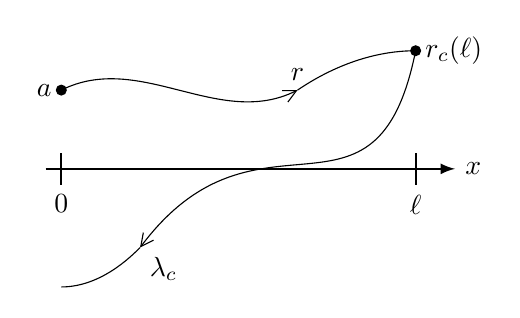
\begin{tikzpicture}
    \draw [thick,->] (-0.2,0) -- (5,0) node [anchor=west] {$x$};
    \draw [thick] (0,0.2) -- (0,-0.2) node [anchor=north] {$0$};
    \draw [thick] (4.5,0.2) -- (4.5,-0.2) node [anchor=north] {$\ell$};
    
    \node [dot] at (0,1) {};
    \node [dot] at (4.5,1.5) {};
    \draw [->,>={Straight Barb[scale length=2]}] (0,1) node [anchor=east] {$a$} .. controls (1,1.5) and (2,0.5) .. (3,1) node [anchor=south] {$r$};
    \draw (3,1) parabola [bend at end] (4.5,1.5) node [anchor=west] {$r_c(\ell)$};

    \draw [->,>={Straight Barb[scale length=2]}] (4.5,1.5) .. controls (4,-1) and (2.5,1) .. (1,-1) node [anchor=north west] {$\lambda_c$};
    \draw (1,-1) parabola [bend at end] (0,-1.5);
  \end{tikzpicture}
\end{center}
Problem: we can do this for any $c$. Which $c$ is it? \emph{Last 15 minutes was a dead end!}

Back to $u=F(r,\lambda)$. Assume we have $F$ (numerically).
\begin{align}
  \frac{\dif r}{\dif x} &= -F(r,\lambda) \\
  r(0) &= a \\
  \frac{\dif\lambda}{\dif x} &= -\frac{F^3(r,\lambda)}{1+F^2(r,\lambda)} \\
  \lambda(\ell) &= r(\ell)
\end{align}
The mistake before was that the simulation forward from $a$ depends on $\lambda$. 
\begin{center}
  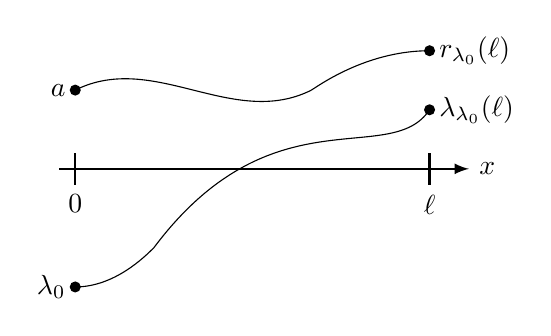
\begin{tikzpicture}
    \draw [thick,->] (-0.2,0) -- (5,0) node [anchor=west] {$x$};
    \draw [thick] (0,0.2) -- (0,-0.2) node [anchor=north] {$0$};
    \draw [thick] (4.5,0.2) -- (4.5,-0.2) node [anchor=north] {$\ell$};
    
    \node [dot] at (0,1) {};
    \node [dot] at (4.5,1.5) {};
    \draw [>={Straight Barb[scale length=2]}] (0,1) node [anchor=east] {$a$} .. controls (1,1.5) and (2,0.5) .. (3,1);
    \draw (3,1) parabola [bend at end] (4.5,1.5) node [anchor=west] {$r_{\lambda_0}(\ell)$};

    \node [dot] at (0,-1.5) {};
    \node [dot] at (4.5,0.75) {};
    \draw [>={Straight Barb[scale length=2]}] (4.5,0.75) node [anchor=west] {$\lambda_{\lambda_0}(\ell)$} .. controls (4,0) and (2.5,1) .. (1,-1);
    \draw (1,-1) parabola [bend at end] (0,-1.5) node [anchor=east] {$\lambda_0$};
  \end{tikzpicture}
\end{center}
Therefore, we should guess $\lambda_0$ and simulate both $r$ and $\lambda$ to get $r_{\lambda_0}(\ell)$ and $\lambda_{\lambda_0}(\ell)$. We need
\[ r_{\lambda_0}(\ell) = \lambda_{\lambda_0} \]
for optimality. To do this, we need numerics.

% 2017/02/09
\paragraph{Terminal Constraints} \mbox{}
\hypertarget{fixed_term_cons}{}

Let $x=[x_1,\dots,x_n]\trans\in\R^n$ and solve
\begin{align}
  & \min_{u\in\mathcal U} \int_0^T L(x,u,t)\dif t + \Psi(x(T)) \\
  & \text{s.t. } \begin{aligned}[t]
    \dot x &= f(x,u,t) \\
    x(0) &= x_0 \\
    x_i(T) &= x_{iT} \quad \text{given for } i\in\mathcal T \subset \{1,\dots,n\}
  \end{aligned}
\end{align}
First, we augment the cost:
\begin{align}
  \tilde J(u) &= \int_0^T \big[ L + \lambda\trans (f-\dot x) \big] \dif t + \Psi \\
              &= \int_0^T (H-\lambda\trans\dot x) \dif t + \Psi \\
  \tilde J (u+\varepsilon v) - \tilde J(u) &= \int_0^T \left( \varepsilon\pder{H}{u} v + \varepsilon\pder{H}{x}\eta - \varepsilon\lambda\trans\dot\eta \right) \dif t + \varepsilon\pder{\Psi}{x}(x(T))\eta(T) + o(\varepsilon) \\
  \delta\tilde J(u;v) &= \int_0^T \left( \pder{H}{x} + \dot\lambda\trans \right)\eta\dif t + \int_0^T \pder{H}{u}v\dif t \\
              & \qquad + \lambda\trans(0)\eta(0) - \lambda\trans(T)\eta(T) + \pder{\Psi}{x}(x(T))\eta(T)
\end{align}
As always,
\begin{align}
  \dot\lambda &= -\pder{H\trans}{x} \\
  \pder{H}{u} &= 0 \quad \text{(FONC)}
\end{align}
Additionally,
\begin{align}
  \eta(0) &= 0 \\
  \eta_i(T) &= 0 \quad \text{for } i\in\mathcal T
\end{align}
Note that if $x(T)=x_T$ is given, then $x(T)=x(T)+\varepsilon\eta(T)+o(\varepsilon)$, so $\eta(T)=0$. Here, we have $x_i(T)=x_{iT}$ fixed for $i\in\mathcal T$ so $\eta_i(T)=0$ for $i\in\mathcal T$.

For optimality, we want
\begin{gather}
  \left[ -\lambda\trans(T) + \pder{\Psi}{x}(x(T)) \right] \eta(T) = 0 \quad \text{for all \emph{admissible} variations} \\
  \begin{bmatrix}
    \displaystyle \pder{\Psi}{x_1}-\lambda_1, & \cdots, & \displaystyle \pder{\Psi}{x_n}-\lambda_n
  \end{bmatrix}
  \begin{bmatrix}
    \eta_1(T) \\
    \vdots \\
    \eta_n(T)
  \end{bmatrix} = 0
\end{gather}
Hence, we need
\begin{alignat}{2}
  \lambda_j(T) &= \pder{\Psi}{x_j}(x(T)) \quad & \text{if } j\not\in\mathcal T \\
  \lambda_i(T) &= \text{free} & \text{if } i\in\mathcal T
\end{alignat}
So we have
\[ \begin{dcases}
    \dot x = f \\
    \dot\lambda = -\pder{H\trans}{x},
  \end{dcases} \]
an ODE with $2n$ variables. We need $2n$ boundary conditions for this ODE to be well-posed.
\begin{center}
  \begin{tabular}{lclc}
    \toprule
    \multicolumn{2}{c}{At $t=0$} & \multicolumn{2}{c}{At $t=T$} \\
    \cmidrule(r){1-2} \cmidrule(l){3-4}
    $x(0)=x_0$ & $[n]$ & $x_i(T)=x_{iT}$, $i\in\mathcal T$ & $[q]$ \\
                                 && $\phantom{x_i(T)=x_{iT}}$ $|\mathcal T|=q$ \\
                                 && $x_j(T)$ free, $j\not\in\mathcal T$ & $[0]$ \\
    $\lambda(0)$ free & $[0]$ & $\lambda_i(T)$ free, $i\in\mathcal T$ & $[0]$ \\
                                 && $\lambda_j(T)=\displaystyle\pder{\Psi}{x_j}(x(T))$, $j\not\in\mathcal T$ & $[n-q]$ \\
    \bottomrule
  \end{tabular}
\end{center}
So we have $n+q+(n-q)=2n$ boundary conditions.

We could even fix some but not all of $x(0)$, i.e.
\begin{alignat}{2}
  x_i(0) &= x_{i0} & \text{if } i\in\mathcal I \\
  x_j(0) &= \text{free} \quad & \text{if } j\not\in\mathcal I
\end{alignat}
Recall,
\[
  \delta\tilde J(u;v) = \int_0^T\! \left(\pder{H}{x} + \dot\lambda\trans \right)\eta\dif t + \int_0^T\! \pder{H}{u} v \dif t + \lambda\trans(0)\eta(0) + \left[\lambda\trans(T)-\pder{\Psi}{x}(x(T))\right] \eta(T)
\]
For $x_i(0)=x_{i0}$ fixed, we have $\eta_i(0)=0$ and $\lambda_i(0)$ free. For $x_j(0)$ free, we have $\eta_j(0)$ free and $\lambda_j(0)=0$.

To ponder, what if $J=\int\! L\dif t + \Psi(x(T)) + \Theta(x(0))$?

To summarize, the minimizer to
\begin{align}
  & \min_{u\in\mathcal U} \int_0^T L(x,u,t)\dif t + \Psi(x(T)) \\
  & \text{s.t. } \begin{aligned}[t]
    \dot x &= f(x,u,t) \\
    x_i(0) &= x_{i0}, \quad i\in\mathcal I \\
    x_j(T) &= x_{jT} \quad j\in\mathcal T
  \end{aligned}
\end{align}
has to satisfy
\begin{align}
  & \pder{H}{u} = 0 \\
  & \dot\lambda = -\pder{H\trans}{x} \\
  & \lambda_i(0) = 0, \quad i\not\in\mathcal I \\
  & \lambda_j(T) = \pder{\Psi}{x_j}(x(T)), \quad j\not\in\mathcal T
\end{align}

\paragraph{Example}
\begin{align}
  & \frac{\dif}{\dif t} \begin{bmatrix}
    x_1 \\ x_2 \\ x_3 \\ x_4
  \end{bmatrix} = f(x_1,x_2,x_3,x_4) \\
  & x_1(0)=1,\, x_3(0)=7,\, x_4(0)=0,\, x_1(1)=2 \\
  & \mathcal I = \{1,3,4\},\, \mathcal T = \{1\} \\
  & \min \int_0^1 L(x,u)\dif t + \big(x_2^2(1) - x_3^2(1) + 7x_1(1) + 14 \big)
\end{align}
Note there are 4 boundary conditions on $x$ so there must be 4 boundary conditions on $\lambda$:
\begin{alignat}{4}
  & \lambda_1(0) \text{ free/unspecified} & \qquad & \lambda_1(1) \text{ free} \\
  & \lambda_2(0) = 0 && \lambda_2(1) = 2x_2(1) \\
  & \lambda_3(0) \text{ free} && \lambda_3(1) = -2x_3(1) \\
  & \lambda_4(0) \text{ free} && \lambda_4(1) = 0
\end{alignat}

\paragraph{Example} \mbox{}

A force $f$ acts on a particle at position $(x,y)$ ($\text{mass}=1$).

\begin{center}
  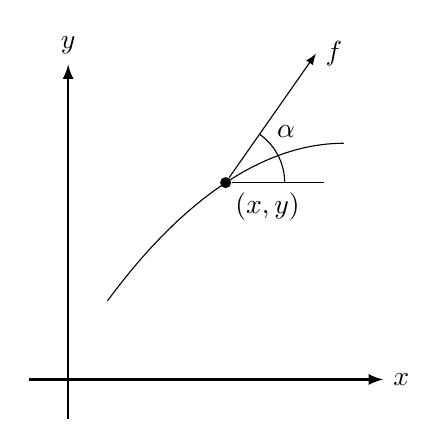
\begin{tikzpicture}
    \draw [thick,->] (-0.5,0) -- (4,0) node [anchor=west] {$x$};
    \draw [thick,->] (0,-0.5) -- (0,4) node [anchor=south] {$y$};
    \draw (0.5,1) parabola [bend at end] (3.5,3);
    \node [dot] (x) at (2,2.5) {};
    \node [anchor=north west] at (x) {$(x,y)$};
    \draw [->] (x) -- ++(55:2) node [anchor=west] {$f$};
    \draw ($(x)+(55:0.75)$) arc (55:0:0.75);
    \node at ($(x)+(40:1)$) {$\alpha$};
    \draw (x) -- ++(1.25,0);
  \end{tikzpicture}
\end{center}
\begin{align}
  \dot x &= v_x \\
  \dot y &= v_y \\
  \dot v_x &= |f|\cos\alpha \\
  \dot v_y &= |f|\sin\alpha \\
  \alpha &= \text{control variable}
\end{align}
Assume we only care about where the particle ends up (to be specified later), i.e.\ $L=0$.
\[
  H = \begin{bmatrix}
    \lambda_x & \lambda_y & \lambda_{v_x} & \lambda_{v_y}
  \end{bmatrix}
  \begin{bmatrix}
    v_x \\ v_y \\ |f|\cos\alpha \\ |f|\sin\alpha
  \end{bmatrix}
\]
\begin{alignat}{3}
  \dot\lambda_x &= -\pder{H}{x} = 0 && \Longrightarrow & \lambda_x(t) &= c_1 \\
  \dot\lambda_y &= -\pder{H}{y} = 0 && \Longrightarrow & \lambda_y(t) &= c_2 \\
  \dot\lambda_{v_x} &= -\pder{H}{v_x} = -\lambda_x && \Longrightarrow & \lambda_{v_x}(t) &= -c_1 t + c_3 \\
  \dot\lambda_{v_y} &= -\pder{H}{v_y} = -\lambda_y \quad && \Longrightarrow & \quad \lambda_{v_y}(t) &= -c_2 t + c_4
\end{alignat}
Moreover,
\begin{align}
  \pder{H}{\alpha} &= -\lambda_{v_x} |f| \sin\alpha + \lambda_{v_y} |f| \cos\alpha = 0 \\
  \tan\alpha &= \frac{\lambda_{v_y}}{\lambda_{v_x}} = \frac{-c_2t+c_4}{-c_1t+c_3}
\end{align}
We want to drive the particle from $[0,0,0,0]\trans$ to a path parallel to the x-axis with $y(T)=h$.

\begin{center}
  \begin{tikzpicture}
    \draw [thick,->] (-0.5,0) -- (5.5,0) node [anchor=west] {$x$};
    \draw [thick,->] (0,-0.5) -- (0,3) node [anchor=south] {$y$};
    \draw [thick] (0.2,2) -- (-0.2,2) node [anchor=east] {$h$};
    \draw (0,0) parabola [bend at end] (3.5,2) -- ++(0.5,0) coordinate (x);
    \node [dot] at (x) {};
    \node [anchor=south] at (x) {$t=T$};
  \end{tikzpicture}
\end{center}
Choose $\Psi=-v_x$,
\begin{alignat}{2}
  y(T) &= h & v_y(T) &= 0 \\
  x(T) & \text{ free} \quad & v_x(T) &\phantom{x} \text{free, but costs} \\
  \lambda_i(0) & \text{ free} \\
  \lambda_y(T) & \text{ free} & \lambda_{v_y}(T) & \text{ free} \\
  \lambda_x(T) &= 0 & \lambda_{v_x}(T) &= -1
\end{alignat}
\begin{align}
  c_1 &= \lambda_x(t) = 0 \\
  \Longrightarrow \lambda_{v_x} &= -c_1t + c_3 = c_3 = -1 \\
  \Longrightarrow \tan\alpha &= -\frac{-c_2t+c_4}{-1} = c_2t + c_4
\end{align}
How do we find $c_2$ and $c_4$? Plug into $\dot x$ and $\dot\lambda$ and try to satisfy the remaining boundary conditions. (This is hard=numerics.)

% 2017/02/14
\section{Splines}
\emph{From ship building.}
Splines are used a lot in path-planning, e.g. cubic splines.
\begin{center}
  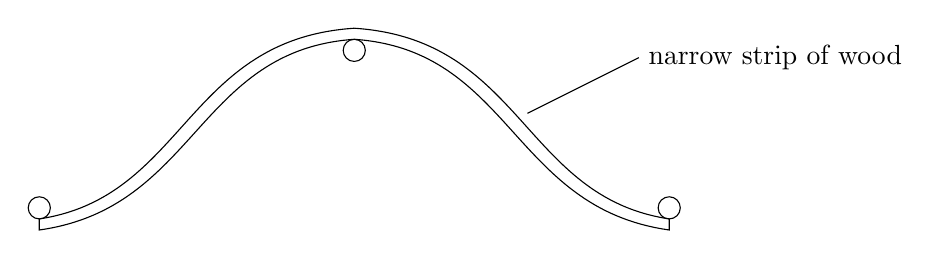
\begin{tikzpicture}[x=2cm,y=1cm]
    \draw (0,0) circle (4pt);
    \draw (2,2) circle (4pt);
    \draw (4,0) circle (4pt);
    \draw ([yshift=-4pt]0,0) .. controls ([xshift=-4pt,yshift=4pt]1,0) and ([xshift=-4pt,yshift=4pt]1,2) .. ([yshift=8pt]2,2);
    \draw ([yshift=-4pt]0,0) -- ([yshift=-8pt]0,0) .. controls (1,0) and (1,2) .. ([yshift=4pt]2,2);
    \draw ([yshift=-4pt]4,0) -- ([yshift=-8pt]4,0) .. controls (3,0) and (3,2) .. ([yshift=4pt]2,2);
    \draw ([yshift=-4pt]4,0) .. controls ([xshift=4pt,yshift=4pt]3,0) and ([xshift=4pt,yshift=4pt]3,2) .. ([yshift=8pt]2,2);
    \draw (3.1,1.2) -- ++(45:1) node [anchor=west] {narrow strip of wood};
  \end{tikzpicture}
\end{center}
But, they are solutions to optimal control problems.

Let $p(t)$ be a curve we'd like to shape.
\pgfmathsetseed{11}
\begin{center}
  \begin{tikzpicture}
    \def\x{0.4}
    \def\dy{0.3}
    \draw [->,thick] (-0.5,0) -- (5,0) node [anchor=west] {$t$};
    \draw [->,thick] (0,-0.5) -- (0,3);
    \draw (0,1) sin (\x,1+\dy) cos (2*\x,1) sin (3*\x,1-\dy) cos (4*\x,1)
    sin (5*\x,1+\dy) cos (6*\x,1) sin (7*\x,1-\dy*2/3) cos (9*\x,1+\dy*2)
    sin (10*\x,1+\dy*3) cos (10.5*\x,1+\dy*2.7) node [anchor=west] {$p(t)$};
  \end{tikzpicture}
\end{center}
We want to minimize the ``energy'' put into the curve, a.k.a\ acceleration.
Let $x_1=p$ and $x_2=\dot p$, so
\[ \begin{cases}
    \dot x_1 = x_2 \\
    \dot x_2 = u
  \end{cases} \]

\subsection{Minimum-Energy}

\begin{align}
  & \min_{u\in\mathcal U} \frac{1}{2} \int_0^T u^2(t)\dif t \quad \text{+ Boundary conditions on $x$} \\
  H &= L+\lambda\trans f = \frac12 u^2 + \lambda_1 x_2 + \lambda_2 u \\
  \pder{H}{u} &= u + \lambda_2 = 0 \Longrightarrow u = -\lambda_2 \\
  \dot\lambda_1 &= -\pder{H}{x_1} = 0 \Longrightarrow \lambda_1 = c_1 \\
  \dot\lambda_2 &= -\pder{H}{x_2} = -\lambda_1 \Longrightarrow \lambda_2 = -c_1t+c_2 \\
  u &= -\lambda_2 = c_1t-c_2 \\
  \dot x_2 &= u = c_1t-c_2 \Longrightarrow x_2 = c_1 \frac{t^2}{2} - c_2t + c_3 \\
  \dot x_1 &= x_2 = c_1\frac{t^2}{2} -c_2t + c_3 \\
  & \Longrightarrow x_1 = \frac{c_1}{6}t^3 - \frac{c_2}{2}t^2 + c_3 t + c_4
\end{align}
$p(t)$ is a cubic polynomial!

\medskip \noindent
What about boundary conditions?

Let $T=1$, $p(0)$ given, $p(1)$ given, $\dot p(0)=0$, $\dot p(1)=0$, e.g.\ $p(0)=0$, $p(1)=1$. Since the boundary conditions for $x$ are all specified, those for the costate are free.
\[
  \left.
    \begin{aligned}
      x_1(0) &= 0 \\
      x_2(0) &= 0 \\
      x_1(1) &= 1 \\
      x_2(1) &= 0
    \end{aligned} \right\}
  \Longrightarrow
  \left\{
    \begin{aligned}
      \lambda_1(0) \\
      \lambda_2(0) \\
      \lambda_1(1) \\
      \lambda_2(1)
    \end{aligned} \right.
  \quad \text{free/unspecified}
\]
\begin{alignat}{2}
  x_2(0) &= c_3 = 0 & x_1(1) &= \frac{2c_2}{6} - \frac{c_2}{2} = 1 \\
  x_1(0) &= c_4 = 0 & c_2 &= -6 \\
  x_2(1) &= \frac{c_1}{2} - c_2 + \smash{ \underbrace{c_3}_{0} } = 0 & c_1 &= -12 \\
  c_1 &= 2c_2
\end{alignat}
\begin{align}
  \Longrightarrow \; & p(t) = -2t^3 + 3t^2 \\
                     & u(t) = -12t + 6
\end{align}

Or, what if $\dot p(0)$, $\dot p(1)$ are not specified?
\[
  \left.
    \begin{aligned}
      x_1(0) &= 0 \\
      x_2(0) & \text{ unspec.} \\
      x_1(1) &= 1 \\
      x_2(1) & \text{ unspec.}
    \end{aligned} \right\}
  \Longrightarrow
  \left\{
    \begin{aligned}
      & \lambda_1(0) \text{ unspec.} \\
      & \lambda_2(0) = 0 \\
      & \lambda_1(1) \text{ unspec.} \\
      & \lambda_2(1) = 0
    \end{aligned} \right.
\]
\begin{align}
  \left.
  \begin{aligned}
    \lambda_2(0) &= c_2 = 0 \\
    \lambda_2(1) &= -c_1 + c_2 = 0
  \end{aligned}
                   \right\} & \Longrightarrow
                              u = c_1t- c_2 = 0 \\
  \left.
  \begin{aligned}
    x_1(0) = c_4 = 0 \\
    x_1(1) = c_3 = 1
  \end{aligned}
  \right\} & \Longrightarrow
             p(t) = t
\end{align}

\noindent
What did we do?
\begin{enumerate}[label=Case \arabic*:,itemindent=1cm]
\item \mbox{}
  \begin{gather}
    \begin{bmatrix}
      0 & 0 & 0 & 1 \\
      1/6 & -1/2 & 1 & 1 \\
      0 & 0 & 1 & 0 \\
      1/2 & -1 & 1 & 0
    \end{bmatrix}
    \begin{bmatrix}
      c_1 \\ c_2 \\ c_3 \\ c_4
    \end{bmatrix}
    =
    \begin{bmatrix}
      0 \\ 1 \\ 0 \\ 0
    \end{bmatrix}
    =
    \begin{bmatrix}
      x_1(0) \\ x_1(1) \\ x_2(0) \\ x_2(1)
    \end{bmatrix}
  \end{gather}
\item \mbox{}
  \begin{gather}
    \begin{bmatrix}
      0 & 0 & 0 & 1 \\
      1/6 & -1/2 & 1 & 1 \\
      0 & 1 & 0 & 0 \\
      -1 & 1 & 0 & 0
    \end{bmatrix}
    \begin{bmatrix}
      c_1 \\ c_2 \\ c_3 \\ c_4
    \end{bmatrix}
    =
    \begin{bmatrix}
      0 \\ 1 \\ 0 \\ 0
    \end{bmatrix}
    =
    \begin{bmatrix}
      x_1(0) \\ x_1(1) \\ \lambda_2(0) \\ \lambda_2(1)
    \end{bmatrix}
  \end{gather}
\end{enumerate}

\subsection{Generalized Splines}
We had $\dot x=Ax+Bu$ with
\[ A = \begin{bmatrix}
    0 & 1 \\ 0 & 0
  \end{bmatrix}. \]
This $A$ is nilpotent ($A^k=0$ for some $k\in\mathbb Z^+$). This means $e^{At}$ is a polynomial in $t$. (This $e^{At}$ is cubic.)

In general, $e^{At}$ is a mix of polynomials, exponentials, and trignometric terms. The eigenvalues of $A$ determine the form of $x(t)$.
\begin{alignat}{3}
  \dot x &= Ax && \Longrightarrow & \; x(t) &= e^{At} x(0) \\
  \dot x &= Ax + Bu && \Longrightarrow & x(t) &= e^{At} x(0) + \int_0^t e^{A(t-\tau)} Bu(\tau) \dif\tau
\end{alignat}
The general problem to solve is
\begin{align}
  & \min_{u\in\mathcal U} \int_0^T \frac{1}{2} \Vert u\Vert^2 \dif t \\
  & \text{s.t. } \dot x = Ax + Bu \\
  & \quad \text{+ Boundary conditions}
\end{align}
\begin{align}
  H &= \frac{1}{2} \Vert u\Vert^2 + \lambda\trans (Ax+Bu) \\
  \pder{H}{u} &= u\trans + \lambda\trans B = 0 \\
    & \Rightarrow u = -B\trans\lambda \\
  \dot\lambda &= -\pder{H\trans}{x} = -A\trans\lambda
\end{align}
We have the Hamiltonian Dynamics:
\begin{gather}
  \begin{bmatrix}
    \dot x \\ \dot\lambda
  \end{bmatrix} =
  \underbrace{
    \begin{bmatrix}
      A & -BB\trans \\
      0 & -A\trans
    \end{bmatrix}
  }_{M}
  \begin{bmatrix}
    x \\ \lambda
  \end{bmatrix}
\end{gather}
Where we used $\dot x=Ax+Bu=Ax-BB\trans\lambda$. Then,
\begin{gather}
  \begin{bmatrix}
    x(t) \\ \lambda(t)
  \end{bmatrix} =
  e^{Mt}
  \begin{bmatrix}
    x(0) \\ \lambda(0)
  \end{bmatrix}
\end{gather}
Suppose we want to drive from $x(0)=x_0$ to $x(T)=x_T$.
\begin{gather}
  \begin{bmatrix}
    x_T \\ \lambda(T)
  \end{bmatrix} =
  e^{MT}
  \begin{bmatrix}
    x_0 \\ \lambda(0)
  \end{bmatrix} =
  \begin{bmatrix}
    N_{xx} & N_{x\lambda} \\
    N_{\lambda x} & N_{\lambda\lambda}
  \end{bmatrix}
  \begin{bmatrix}
    x_0 \\ \lambda(0)
  \end{bmatrix} \\
  x_T = N_{xx} x_0 + N_{x\lambda} \lambda(0) \\
  \intertext{$N_{x\lambda}$ is invertible if $(A,B)$ is completely controllable. Assume it is.}
  \lambda(0) = N_{x\lambda}^{-1} (x_T - N_{xx} x_0) \\
  \Longrightarrow
  \begin{bmatrix}
    x(t) \\ \lambda(t)
  \end{bmatrix} =
  e^{Mt}
  \begin{bmatrix}
    x_0 \\
    N_{x\lambda}^{-1} (x_T - N_{xx} x_0)
  \end{bmatrix} \\
  \Longrightarrow u(t) = -B\trans \lambda(t)
\end{gather}
This is the optimal trajectory, but there is no feedback. We will consider closed-loop systems after the midterm.

As a preview, we need to find $\lambda$ as a function of $x$. For example, $u=-R^{-1} B\trans Px$ minimizes $u\trans Ru$, so $\lambda=Px$ where $P$ is the solution to the Riccati equation.

% 2017/02/16
\section{Numerical Methods}
Optimal control boils down to solving two sets of differential equations:
\begin{gather}
  \begin{aligned}
    \dot x &= f(x,u) & \quad & \pder{H}{u}(x,u,\lambda) = 0 \\
    \dot\lambda &= -\pder{H\trans}{x}(x,u,\lambda) && u = F(x,\lambda) \\
  \end{aligned} \\
  \Longrightarrow \begin{dcases}
    \dot x = f(x,F(x,\lambda)) \\
    \dot \lambda = -\pder{H\trans}{x}(x,F(x,\lambda),\lambda)
  \end{dcases}
\end{gather}
The equations are functions of $x$ and $\lambda$. They are completely determined by the boundary conditions on $x(0)$, $x(T)$, $\lambda(0)$, $\lambda(T)$. This is known as the \emph{Boundary Value Problem}. This is solved using \emph{test shooting}:
\begin{enumerate}
\item Guess initial conditions
\item Simulate forward in time
\item Update the guess (cleverly\dots)
\end{enumerate}

\paragraph{Exmaple:} Bolza problem
\begin{align}
  & \min_{u\in\mathcal U} \int_0^T L(x,u)\dif t + \Psi(x(T)) \\
  & \text{s.t. } \begin{cases}
    \dot x=f(x,u) \\
    x(0) = x_0
  \end{cases} \\
  & H(x,u,\lambda) = L(x,u) + \lambda\trans f(x,u) \\
  & u^* (x,\lambda) \text{ satisfies } \pder{H}{u} = 0
\end{align}
The optimal control satisfies
\begin{gather}
  \begin{dcases}
    x = f(x,u^*(x,\lambda)) \\
    x(0) = x_0 \\
    \lambda = -\pder{H\trans}{x} (x,u^*(x,\lambda),\lambda) \\
    \lambda(T) = \pder{\Psi}{x}(x(T))
  \end{dcases}
\end{gather}

\paragraph{Algorithm}
Guess $\lambda_0$ and solve for $x(t)$, $\lambda(t)$.
\begin{center}
  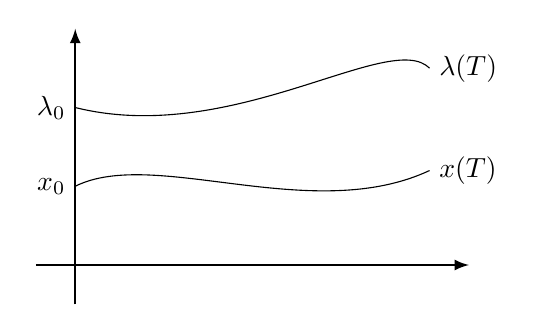
\begin{tikzpicture}
    \draw [thick,->] (-0.5,0) -- (5,0);
    \draw [thick,->] (0,-0.5) -- (0,3);
    \draw (0,1) node [anchor=east] {$x_0$} .. controls (1,1.5) and (3,0.5) .. (4.5,1.2) node [anchor=west] {$x(T)$};
    \draw (0,2) node [anchor=east] {$\lambda_0$} .. controls (2,1.5) and (4,3) .. (4.5,2.5) node [anchor=west] {$\lambda(T)$};
  \end{tikzpicture}
\end{center}
Let's define a cost:
\[ \left\Vert \lambda(T) - \pder{\Psi\trans}{x}(x(T)) \right\Vert^2 = g(\lambda_0) \]
Update $\lambda_0$ through
\[ \lambda_0 \coloneqq \lambda_0 - \underset{\mathclap{\substack{\big\uparrow\\ \text{\normalsize any choice of step size works}}}}{\gamma} \pder{g\trans}{\lambda_0}(\lambda_0) \]
Repeat

\medskip

\noindent
Problem: What is $\partial g/\partial\lambda_0$? We estimate $\partial g/\partial\lambda_0$ numerically. This is where ``test shooting'' comes into play.

Let $e_i$ be the $i$th unit vector, $i=1,\dots,n$:
\begin{gather}
  e_1 = \begin{bmatrix}
    1 \\ 0 \\ \vdots \\ 0
  \end{bmatrix}\!,\ 
  e_2 = \begin{bmatrix}
    0 \\ 1 \\ \vdots \\ 0
  \end{bmatrix}\!,\ 
  \dots,\ 
  e_n = \begin{bmatrix}
    0 \\ 0 \\ \vdots \\ 1
  \end{bmatrix} \\
  \pder{g}{\lambda_0} = \left( \pder{g}{\lambda_{0,1}},\pder{g}{\lambda_{0,2}},\dots,\pder{g}{\lambda_{o,n}} \right)
\end{gather}
The $i$th component of $\partial g/\partial\lambda_0$ is given by the directional derivative
\[
  \pder{g}{\lambda_{0,i}} = \pder{g}{\lambda_0} \cdot e_i = \delta g(\lambda_0;e_i) = \lim_{\varepsilon\to0} \frac{g(\lambda_0+\varepsilon e_i) - g(\lambda_0)}{\varepsilon}
\]
So, if $x\in\R^n$ (and thus so is $\lambda_0$), we have to do this $n$ times (with a small $\varepsilon$) and get the full derivative $\partial g/\partial\lambda_0$.

\paragraph{Algorithm} \mbox{}
\begin{algorithm}
  \begin{algorithmic}
    \State Given $\lambda_0$, $g(\lambda_0)$
    \For {$i=1$ to $n$}
    \State Compute $g(\lambda_0+\varepsilon e_i)$
    \State $dg_i = \dfrac{1}{\varepsilon} [g(\lambda_0+\varepsilon e_i) - g(\lambda_0)]$
    \EndFor
    \smallskip
    \State $\displaystyle\pder{g}{\lambda_0} = [dg_1,\dots,dg_n]$
  \end{algorithmic}
\end{algorithm}

\paragraph{Example} LQ
\begin{align}
  & \min_u \frac12 \int_0^1 (x\trans Qx + u\trans Ru) \dif t + \frac12 x\trans(1)Sx(1) \\
  & \text{s.t. } \begin{dcases}
    \dot x = Ax + Bu \\
    x(0) = x_0
  \end{dcases} \\
  & \phantom{\text{s.t. }} Q,R,S \succ 0
\end{align}
\begin{align}
  H &= \frac12 x\trans Qx + \frac12 u\trans Ru + \lambda\trans(Ax+Bu) \\
  \pder{H}{u} &= u\trans R + \lambda\trans B = 0 \\
  u^* &= -R^{-1}B\trans \lambda \\
  \dot\lambda &= -\pder{H\trans}{x} = -Qx - A\trans\lambda \\
  \lambda(1) &= \pder{\Psi\trans}{x}(x(1)) = Sx(1)
\end{align}
So putting it all together,
\begin{alignat}{2}
  \dot x &= Ax - BR^{-1}B\trans\lambda \qquad & x(0) &= x_0 \\
  \dot\lambda &= -Qx - A\trans\lambda & \lambda(1) &= Sx(1)
\end{alignat}

\paragraph{Example} Newton's nose shape problem (\hyperlink{newton_nose_shape}{revisited, see previous})

\begin{align}
  & \min_u \int_0^\ell \frac{ru^3}{1+u^2}\dif x + \frac12 r(\ell)^2 \\
  & \text{s.t. } \frac{\dif r}{\dif x} = -u \qquad r(0) = a
\end{align}
\begin{align}
  H &= \frac{ru^3}{1+u^2} + \lambda(-u) \\
  \pder{H}{u} &= \frac{ru^2(3+u^2)}{(1+u^2)^2} - \lambda = 0 \\
  \shortintertext{We solve the above numerically to get $u^*(r,\lambda)$.}
  \pder{\lambda}{x} &= -\pder{H}{r} = -\frac{u^3}{1+u^2} \\
  \lambda(\ell) &= r(\ell)
\end{align}
So, we have
\begin{alignat}{3}
  \frac{\dif r}{\dif x} &= -u & r(0) &= a & u &= F(x,\lambda) \\
  \frac{\dif\lambda}{\dif x} &= -\frac{u^3}{1+u^2} \qquad & \lambda(\ell) &= r(\ell) \qquad
\end{alignat}

\paragraph{Example} Fixed terminal constraints (\hyperlink{fixed_term_cons}{revisited, see previous})

\begin{align}
  & \min_\alpha -v_x(T) \qquad \alpha=\text{control} \\
  & \text{s.t. } \begin{aligned}[t]
    \dot x &= v_x & x(0) &= 0 \\
    \dot y &= v_y & y(0) &= 0 \\
    \dot v_x &= |f|\cos\alpha & v_x(0) &= 0 \\
    \dot v_y &= |f|\sin\alpha & v_y(0) &= 0 \\
    y(T) &= h \\
    v_y(T) &= 0
  \end{aligned}
\end{align}
\begin{align}
  H &= -v_x(T) + \begin{bmatrix}
    \lambda_x & \lambda_y & \lambda_{v_x} & \lambda_{v_y}
  \end{bmatrix}
                                            \begin{bmatrix}
                                              v_x \\ v_y \\ |f|\cos\alpha \\ |f|\sin\alpha
                                            \end{bmatrix} \\
  \frac{\dif H}{\dif\alpha} &= 0 \Rightarrow \tan\alpha = \frac{\lambda_{v_y}}{\lambda_{v_x}} \\
  \dot\lambda_x &= 0 \\
  \dot\lambda_y &= 0 \\
  \dot\lambda_{v_x} &= -\lambda_x \\
  \dot\lambda_{v_y} &= -\lambda_y \\
  \bm\lambda(0) & \text{ unspecified} \\
  \lambda_x(T) &= \pder{\Psi\trans}{x}(x(T)) = 0 \\
  \lambda_y(T) & \text{ unspecified} \\
  \lambda_{v_x}(T) &= \pder{\Psi\trans}{v_x}(v_x(T)) = -1 \\
  \lambda_{v_y}(T) & \text{ unspecified}
\end{align}
Again, we guess $\lambda_0$ and solve forward in time. But, we have terminal constraints on $y$ and $v_y$ as well.
\begin{gather}
  g(\lambda_0) = \frac12 \Big[ (y(T)-h)^2 + (v_y(T))^2 + (\lambda_x(T))^2 + (\lambda_{v_x}+1)^2 \Big]
\end{gather}

% 2017/02/28

\section{Terminal Manifolds}

We can solve
\begin{align}
  & \min_{u\in\mathcal U} \int_0^T L(x,u,t)\dif t + \Psi(x(T)) \\
  & \text{s.t. } \dot x = f(x,u,t)
\end{align}
with all sorts of boundary conditions on $x$:
\begin{itemize}
\item $x(0)=x_0$, $x(T)$ free (typical)
\item $x_i(0)=x_{i0}$, $i\in\mathcal I$ and $x_j(T)=x_{jT}$, $j\in\mathcal T$
\end{itemize}
But what if we want $x(T)$ to belong to a set?

\begin{center}
  \begin{tikzpicture}
    \draw (0,0) coordinate (a) .. controls (1.5,0.5) and (2,-0.5) .. (4,-1) coordinate (b);
    \node [dot] at (a) {};
    \node [dot] at (b) {};
    \node [below left] at (a) {$x_0$};
    \node [right] at (b) {$x(T)$};
    \draw (b) arc (-160:200:0.75cm and 1.25cm);
    \node [right] at ($(b)+(1.5,0.5)$) {$\phi=0$};
  \end{tikzpicture}
\end{center}

\paragraph{Problem}
\begin{align}
  & \min_{u\in\mathcal U} \int_0^T L(x,u,t)\dif t + \Psi(x(T)) \\
  & \text{s.t. } \begin{aligned}[t]
    & \dot x = f(x,u,t), && x\in\R^n \\
    & x(0) = x_0 \\
    & \phi(x(T)) = 0, && \phi:\R^n\to\R^q,\ q\le n
  \end{aligned}
\end{align}
The augmented cost is
\[
  \tilde J = \int_0^T [ H(x,u,t,\lambda) - \lambda\trans \dot x]\dif t + \Psi(x(T)) + \underset{\mathclap{\substack{\uparrow\\ \text{q-dimensional}\\ \text{Lagrange multiplier}}}}{\nu}\trans \phi(x(T))
\]
Let $\Phi(x(T),\nu)=\Psi(x(T)) + \nu\trans\phi(x(T))$. Then,
\[
  \tilde J = \int_0^T \left( \pder{H}{x} + \dot\lambda\trans \right) \eta \dif t + \Phi(x(T),\nu)
\]
We know how to solve this! With $u\mapsto u+\varepsilon v$, $x\mapsto x+\varepsilon\eta + o(\varepsilon)$,
\begin{align}
  \delta \tilde J &= \int_0^T \left(\pder{H}{x} + \dot\lambda\trans\right)\eta\dif t + \int_0^T \pder{H}{u}v \dif t + \pder{\Phi}{x}(x(T),\nu)\eta(T) \\
                  & \qquad - \lambda\trans(T)\eta(T) + \lambda\trans(0)\underbracket{\eta(0)}_{=0} \\
                  & \begin{dcases}
                    \pder{H}{u} = 0 \\
                    \dot\lambda = -\pder{H\trans}{x} \\
                    \lambda(T) = \pder{\Phi\trans}{x}( x(T), \overset{\mathclap{\substack{q \text{ new variables}\\ \downarrow}}}{\nu} ) \\
                    \phi(x(T)) = 0 \ \leftarrow q \text{ new equations}
                  \end{dcases} \\
                  & \Longrightarrow u^*
\end{align}

\paragraph{Spling to line}

\begin{align}
  & \min_u \frac12 \int_0^1 u^2(t) \dif t \\
  & \text{s.t. } \adjustbox{valign=t}{$\begin{dcases}
      \dot x_1 = x_2 \\
      \dot x_2 = u \\
      x_1(0) = 0,\ x_2(0) = 0 \\
      c_1 x_1(1) + c_2 x_2(1) = d
    \end{dcases}$}
\end{align}

\begin{center}
  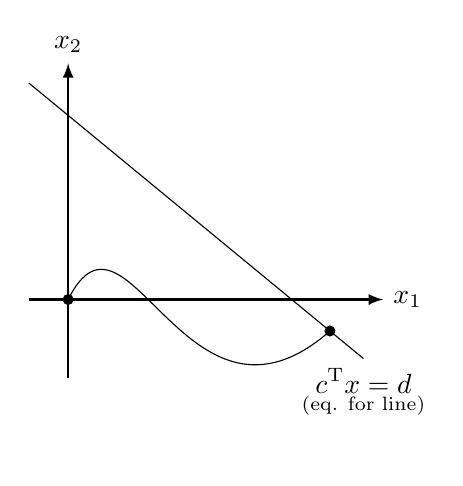
\begin{tikzpicture}
    \draw [thick,->] (-0.5,0) -- (4,0) node [right] {$x_1$};
    \draw [thick,->] (0,-1) -- (0,3) node [above] {$x_2$};
    \draw (-0.5,2.75) coordinate (a) -- (3.75,-0.75) coordinate (b) node [below] {$\substack{\displaystyle c\trans x=d\\ \text{(eq. for line)}}$};
    \draw (0,0) coordinate (o) .. controls (0.75,1.5) and (1.5,-2) .. ($(b)!0.1!(a)$) coordinate (c);
    \node [dot] at (o) {};
    \node [dot] at (c) {};
  \end{tikzpicture}
\end{center}

\begin{align}
  H &= \frac12 u^2 + \lambda_1 x_2 + \lambda_2 u \\
  \pder{H}{u} &= u + \lambda_2 \Longrightarrow u = -\lambda_2 \\
  \dot\lambda_1 &= -\pder{H}{x_1} = 0 \Longrightarrow \lambda_1 = k_1 \\
  \dot\lambda_2 &= -\pder{H}{x_2} = -\lambda_1 \Longrightarrow \lambda_2 = -k_1 t + k_2 \\
  \phi(x(1)) &= c_1 x_1(1) + c_2 x_2(1) - d \\
  \Psi &= 0 \Longrightarrow \Phi = \nu (c_1x_1(1) + c_2x_2(1) - d) \\
  \lambda_1(1) &= \pder{\Phi}{x_1} = \nu c_1 \\
  \lambda_2(1) &= \pder{\Phi}{x_2} = \nu c_2 \\
  \shortintertext{So,}
  \lambda_1(1) &= \nu c_1 = k_1 \\
  \lambda_2(1) &= \nu c_2 = -k_1 + k_2 \\
  k_2 &= \nu (c_1 + c_2) \\
  \dot x_2 &= u = -\lambda_2 = k_1 t - k_2 \\
  x_2 &= \frac{k_1}{2} t^2 - k_2 t + 0 \\
  \dot x_1 &= x_2 \\
  x_1 &= \frac{k_1}{6} t^3 - \frac{k_2}{2} t^2 + 0 \\
  \shortintertext{Substituting $k_1$ and $k_2$ into $c_1x_1(1)+c_2x_2(1)=d$,}
    & \nu \left( -\frac{c_1^2}{3} - c_1 c_2 - c_2^2 \right) = d \\
  \nu &= - \frac{d}{c_1^2/3 + c_1c_2 + c_2^2} \\
  \shortintertext{And finally}
  \Aboxed{u &= k_1 t - k_2 = \frac{d}{c_1^2/3 + c_1c_2 + c_2^2} (c_1 + c_2 - c_1 t)}
\end{align}
As a final observation if $\Psi=0$ then
\[
  \lambda(T) = \nu\trans \pder{\phi}{x}(x(T)),
\]
which means $\lambda(T)$ is orthogonal to the tangent plane to $\phi(x(T))$.

\begin{center}
  \begin{tikzpicture}
    \draw (0,0) parabola [bend at end] (1,0.5);
    \draw (1,0.5) parabola (3,-2);
    \draw (3,-2) parabola [bend at end] (3.5,-2.5);
    \draw (3.5,-2.5) -- ++(3,0) node [right] {$\phi=0$};
    \draw [->] (5,-2.5) coordinate (a) -- ++(0,-1.25) coordinate (b);
    \node [below] at (b) {$\lambda(T)$};
    \draw ($(a)!8pt!(b)$) coordinate (c) -- ($(c)!1!-90:(a)$) coordinate (d);
    \draw (d) -- ($(d)!1!-90:(c)$);
    \draw [->] (2.25,-0.48) coordinate (e) -- ++ (33:1.25) coordinate (f);
    \node [right] at (f) {$\lambda(T)$};
    \draw ($(e)!8pt!(f)$) coordinate (g) -- ($(g)!1!90:(e)$) coordinate (h);
    \draw (h) -- ($(h)!1!90:(g)$);
  \end{tikzpicture}
\end{center}

\paragraph{Example} Maximum orbit transform (e.g.\ Hidden Figures)

\bigskip

\begin{tabular}{cc}
  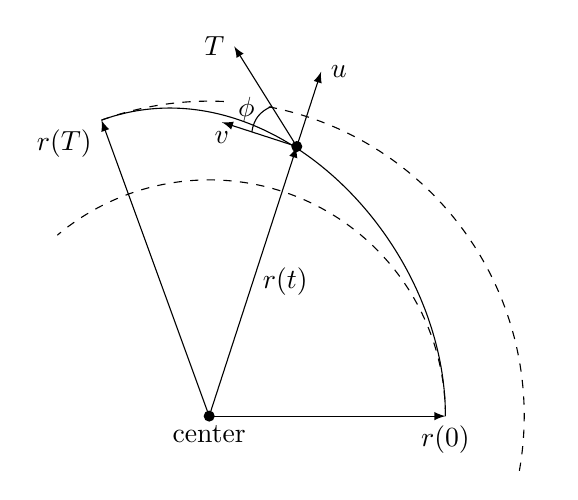
\begin{tikzpicture}[baseline=(c)]
    \node [dot] at (0,0) {};
    \node [below] at (0,0) {center};
    \draw [->] (0,0) -- ++(3,0) coordinate (a);
    \node [below] at (a) {$r(0)$};
    \draw [->] (0,0) -- ++(110:4) coordinate (b);
    \node [below left] at (b) {$r(T)$};
    \draw (a) to [out=90,in=20] (b);
    \draw [dashed] (a) arc (0:130:3);
    % \draw [dashed] (b) arc (110:-10:4);
    \path (b) arc (110:-10:4) coordinate (rT);
    \draw [dashed] (b) arc (110:86:4);
    \draw [dashed] (rT) arc (-10:80:4);

    \draw [->] (0,0) -- ++(72:3.6) coordinate (c) node [pos=0.5,right] {$r(t)$};
    \node [dot] at (c) {};
    \draw [->] (c) -- ($(c)!-1cm!(0,0)$) coordinate (u);
    \node [right] at (u) {$u$};
    \draw [->] (c) -- ($(c)!1!90:(u)$) coordinate (v) node [below] {$v$};
    \draw [->] (c) -- ($(c)!1.5!50:(u)$) coordinate (T) node [left] {$T$};
    \path ($(c)!0.6cm!(v)$) coordinate (vv) ($(c)!0.6cm!(T)$) coordinate (TT);
    \draw (vv) to [bend left] (TT);
    \node [above,xshift=-2pt] at (vv) {$\phi$};
  \end{tikzpicture}
  &
    \begin{tabular}[t]{>{$}r<{$} @{${}={}$} p{6cm}}
      r & radial distance from spacecraft to center \\
      u & radial velocity \\
      v & tangential velocity \\
      m & mass of spacecraft \\
      \dot m & $-$fuel consumption rate \\
      \phi & thrust angle (control input) \\
      T & thrust
    \end{tabular}
\end{tabular}

\begin{align}
  & \max_\phi r(T) \Longleftrightarrow \min_\phi -r(T) \\
  & \text{s.t. } \adjustbox{valign=t}{$\begin{dcases}
      \dot r = u \\
      \dot u = \frac{v^2}{r} - \frac{g}{r^2} + \frac{T\sin\phi}{m_0 - |\dot m|t} \\
      \dot v = -\frac{uv}{r} + \frac{T\cos\phi}{m_0 - |\dot m|t} \\
      r(0) = r_0 \\
      u(0) = 0 \\
      v(0) = \sqrt{\frac{g}{r_0}} \\
      u(T) = 0 = \phi_1 \\
      v(T) = \sqrt{\frac{g}{r(T)}} = \phi_2
    \end{dcases}$}
\end{align}

\begin{align}
  H &= \lambda_r u + \lambda_u \left( \frac{v^2}{r} - \frac{g}{r^2} + \frac{T\sin\phi}{m_0-|\dot m|t} \right) + \lambda_v \left(-\frac{uv}{r} + \frac{T\cos\phi}{m_0-|\dot m|t} \right) \\
  \Phi &= \underbrace{\nu_1 u(T) + \nu_2 \left(v(T) - \sqrt{\frac{g}{r(T)}}\right)}_{\nu\trans\phi} \underbrace{- r(T)}_{\Psi} \\
  \pder{H}{\phi} &= \frac{\lambda_u T\cos\phi - \lambda_v T\sin\phi}{m_0 - |\dot m|t} = 0 \\
    & \Rightarrow \tan\phi = \frac{\lambda_u}{\lambda_v} \\
  \dot\lambda_r &= -\pder{H}{r} = -\lambda_u \left(-\frac{v^2}{r^2} + \frac{2g}{r^3}\right) - \lambda_v\cdot\frac{uv}{r^2} \\
  \dot\lambda_u &= -\pder{H}{u} = -\lambda_r + \lambda_v\cdot \frac{v}{r} \\
  \dot\lambda_v &= -\pder{H}{v} = -\lambda_u\cdot \frac{2v}{r} + \lambda_v\cdot \frac{u}{r} \\
    & \begin{dcases}
      \lambda_r(T) = \pder{\Phi}{r} = -1 + \frac{\nu_2\sqrt{g}}{2(r(T))^{3/2}} \\
      \lambda_u(T) = \pder{\Phi}{u} = \nu_1 \\
      \lambda_v(T) = \pder{\Phi}{v} = \nu_2 \\
      u(T) = 0 \\
      v(T) = \sqrt{\frac{g}{r(T)}}
    \end{dcases}
\end{align}
This needs numerics to solve.

\subsection{Terminal manifold with inequality constraints}
\begin{align}
  & \min_u \int_0^T L\dif t + \Psi \\
  & \dot x = f(x,u) \\
  & \phi(x(T)) \le 0
\end{align}

\begin{center}
  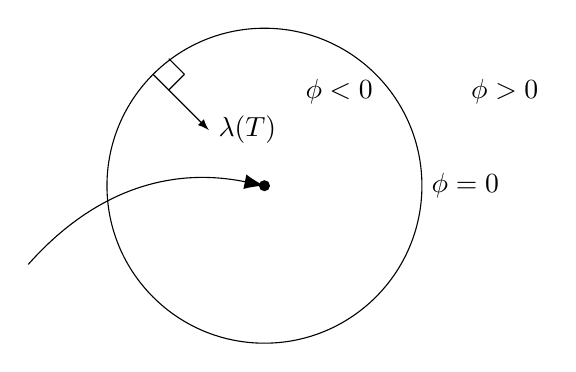
\begin{tikzpicture}
    \node [dot] at (0,0) {};
    \draw [-{Latex[scale=1.5]}] (-3,-1) to [bend left] (0,0);

    \draw (0,0) circle (2);
    \node [right] at (2,0) {$\phi=0$};
    \node [right] at (2.5,1.2) {$\phi>0$};
    \node [left] at (1.5,1.2) {$\phi<0$};

    \path (2,0) arc (0:135:2) coordinate (a);
    \draw [->] (a) -- ++(-45:1) coordinate (b);
    \node [right] at (b) {$\lambda(T)$};
    \draw ($(a)!8pt!(b)$) coordinate (c) -- ($(c)!1!-90:(a)$) coordinate (d);
    \draw (d) -- ($(d)!1!-90:(c)$);
  \end{tikzpicture}
\end{center}

Repeat process: $\tilde J = \int(H-\lambda\trans\dot x)\dif t + \Psi + \nu\trans\phi$. The optimality conditions are
\[
  \begin{dcases}
    \pder{H}{u} = 0 \\
    \dot\lambda = -\pder{H\trans}{x} \\
    \lambda(T) = \pder{\Psi\trans}{x}(x(T)) + \nu\trans\pder{\phi\trans}{x}(x(T)) \\
    \nu \ge 0 \\
    \phi(x(T)) \le 0 \\
    \nu\trans \phi(x(T)) = 0 \quad (\text{KKT})
  \end{dcases}
\]

\subsection{Initial manifold}
\begin{align}
  & \min_{x_0,u} \int L + \Psi(x(T)) + \Theta(x(0)) \\
  & \text{s.t. } \begin{aligned}[t]
    & \dot x = f(x,u) \\
    & \phi(x(T)) = 0 \\
    & \xi(x(0)) = 0
  \end{aligned}
\end{align}

\begin{align}
  \tilde J &= \int (H-\lambda\trans\dot x)\dif t + \Psi(x(T)) + \Theta(x(0)) + \nu\trans_\phi \phi(x(T)) + \nu\trans_\xi \xi(x(0)) \\
  \delta \tilde J &= \int \left[ \left( \pder{H}{x} + \dot\lambda\trans \right) \eta + \pder{H}{u}v\right] \dif t + \left[ \pder{\Psi}{x}(x(T)) + \nu\trans_\phi \pder{\phi}{x}(x(T)) - \lambda\trans(T) \right] \eta(T) \\
           & \qquad + \left[ \pder{\Theta}{x}(x(0)) + \nu\trans_\xi \pder{\xi}{x}(x(0)) + \lambda\trans(0) \right] \eta(0)
\end{align}
The optimality conditions are
\[
  \begin{dcases}
    \pder{H}{u} = 0 \\
    \dot\lambda = -\pder{H\trans}{x} \\
    \lambda(T) = -\pder{\Psi\trans}{x}(x(T)) - \nu\trans_\phi \pder{\phi\trans}{x}(x(T)) \\
    \lambda(0) = -\pder{\Theta\trans}{x}(x(0)) - \nu\trans_\xi \pder{\xi\trans}{x}(x(0))
  \end{dcases}
\]

% 2017/03/02

\subsection{Unspecified Terminal Times}

For example, instead of driving to the moon using minimum fuel, we want to get there as soon as possible:
\[
  \min_{u,T} \int_0^T L(x,u,t)\dif t + \Psi(x(T),T).
\]
The variations are $u\mapsto u+\varepsilon v$ and $T\mapsto T+\varepsilon\tau$

\begin{center}
  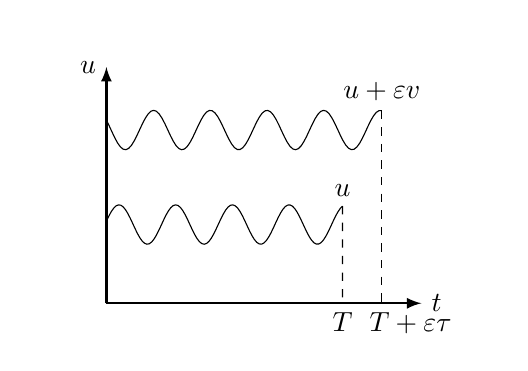
\begin{tikzpicture}
    \clip (-1,-0.5) rectangle (5,3.5);
    \draw [thick,->,name path=x-axis] (0,0) -- (4,0) node [right] {$t$};
    \draw [thick,->] (0,0) -- (0,3) node [left] {$u$};
    \draw [domain=0:3,samples=100] plot(\x,{sin(500*\x + 10)/4 + 1}) coordinate (a) node [above] {$u$};
    \draw [domain=0:3.5,samples=100] plot(\x,{sin(500*\x + 150)/4 + 2.2}) coordinate (b) node [above] {$u+\varepsilon v$};
    \path [name path=u] (a) -- ++(0,-2);
    \path [name path=u2] (b) -- ++(0,-3);
    \draw [dashed,name intersections={of=x-axis and u}] (a) -- (intersection-1) node [below] {$T$};
    \draw [dashed,name intersections={of=x-axis and u2}] (b) -- (intersection-1) node [below right,xshift=-8pt] {$T+\varepsilon\tau$};
  \end{tikzpicture}
  \hspace{1cm}
  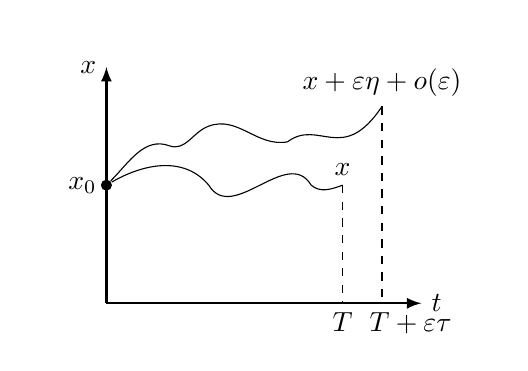
\begin{tikzpicture}
    \clip (-1,-0.5) rectangle (5,3.5);
    \draw [thick,->,name path=x-axis] (0,0) -- (4,0) node [right] {$t$};
    \draw [thick,->] (0,0) -- (0,3) node [left] {$x$};
    \node [dot] (x0) at (0,1.5) {};
    \node [left] at (x0) {$x_0$};
    \draw (x0) to [out=30,in=130] ++(1.3,0) .. controls ++(0.3,-0.5) and (2.3,2) .. (2.6,1.5) to [out=-40,in=200] (3,1.5) coordinate (a) node [above] {$x$};
    \draw (x0) to [out=45,in=160] ++(0.8,0.5) to [out=-20,in=200] ++(0.5,0.25) to [out=20,in=190] ++(1,-0.2) .. controls ++(0.4,0.3) and ++(-0.5,-0.75) .. (3.5,2.5) coordinate (b) node [above] {$x+\varepsilon\eta+o(\varepsilon)$};
    \path [name path=x] (a) -- ++(0,-2);
    \path [name path=x2] (b) -- ++(0,-3);
    \draw [dashed,name intersections={of=x-axis and x}] (a) -- (intersection-1) node [below] {$T$};
    \draw [dashed,name intersections={of=x-axis and x2}] (b) -- (intersection-1) node [below right,xshift=-8pt] {$T+\varepsilon\tau$};
  \end{tikzpicture}
\end{center}

\begin{align}
  \tilde J(u,T) &= \int_0^T [ L(x,u,t) + \lambda\trans(f(x)-\dot x)]\dif t + \Psi(x(T),T) \\
                &= \int_0^T [H - \lambda\trans\dot x]\dif t + \Psi \\
  \tilde J(u+\varepsilon v,T+\varepsilon\tau) &= \int_0^T [H(x+\varepsilon\eta,u+\varepsilon v,t,\lambda) - \lambda\trans(\dot x+\varepsilon\dot\eta)]\dif t \\
                & \qquad + \int_T^{T+\varepsilon\tau} [H(x+\varepsilon\eta,u+\varepsilon v,t,\lambda) - \lambda\trans(\dot x+\varepsilon\dot\eta)]\dif t \\
                & \qquad + \Psi(x(T+\varepsilon\tau)+\varepsilon\eta(T+\varepsilon\tau),T+\varepsilon\tau) \displaybreak \\
  \tilde J(u+\varepsilon v,T+\varepsilon\tau) - \tilde J(u,T) &= \varepsilon \int_0^T \left(\pder{H}{x} + \dot\lambda\trans\right)\eta\dif t + \varepsilon \int_0^T \pder{H}{u}v\dif t \label{eq:unspec_term_time} \\
                & \qquad - \varepsilon\lambda\trans(T)\eta(T) + \varepsilon\lambda\trans(0)\eta(0) + o(\varepsilon) \\
                & \qquad + \underbrace{\int_T^{T+\varepsilon\tau} [H(x+\varepsilon\eta,u+\varepsilon v,t,\lambda) - \lambda\trans(\dot x + \varepsilon\dot\eta)]\dif t}_{\displaystyle\text{(I)}} \\
                & \qquad + \underbrace{\Psi(x(T+\varepsilon\tau)+\varepsilon\eta(T+\varepsilon\tau),T+\varepsilon\tau) - \Psi(x(T),T)}_{\displaystyle\text{(II)}}
\end{align}
For term I, use the mean value theorem to get rid of terms inside the integral that have a $\varepsilon$ before them:
\begin{align}
  \MoveEqLeft \int_T^{T+\varepsilon\tau} [L + \lambda\trans(f-\dot x-\varepsilon\dot\eta)]\dif t \\
&= \int_T^{T+\varepsilon\tau} \left[ L(x,u,t) + \varepsilon\pder{L}{x}\eta + \varepsilon\pder{L}{u}v + \lambda\trans \left( f + \varepsilon\pder{f}{x}\eta + \varepsilon\pder{f}{u}v - \dot x - \varepsilon\dot\eta \right) \right]\dif t + o(\varepsilon) \\
&= \varepsilon\tau \big[ L + \lambda\trans(f-\dot x) \big] \big|_{t=\xi} + o(\varepsilon) = \varepsilon\tau L \big|_{t=\xi} + o(\varepsilon) \\
&= \varepsilon\tau L(x(\xi),u(\xi),\xi) + o(\varepsilon), \quad \xi\in[T,T+\varepsilon\xi] \label{eq:unspec_term_time_I}
\end{align}
Note that as $\varepsilon\to0$, $\xi\to T$.

For term II, we further split it into two parts:
\begin{gather}
  \Psi(x+\varepsilon\eta,T+\varepsilon\tau) - \Psi(x,T) = \underbrace{\Psi(x,T+\varepsilon\tau)}_{\displaystyle\text{(II.a)}} + \underbrace{\varepsilon\pder{\Psi}{x}(x,T+\varepsilon\tau)\eta(T+\varepsilon\tau)}_{\displaystyle\text{(II.b)}} - \Psi(x,T)
\end{gather}
\begin{align}
  \text{(II.a)}\Longrightarrow \Psi(x,T+\varepsilon\tau) &= \Psi(x(T),T+\varepsilon\tau) + \varepsilon\pder{\Psi}{x}(x(T),T+\varepsilon\tau)\dot x(T)\tau + o(\varepsilon) \\
                                                         &= \Psi(x(T),T) + \varepsilon\pder{\Psi}{x}(x(T),T)\dot x(T)\tau + \varepsilon\pder{\Psi}{T}(x(T),T)\tau + o(\varepsilon) \\
  \text{(II.b)}\Longrightarrow \varepsilon\pder{\Psi}{x}(x,T+\varepsilon\tau) & \eta(T+\varepsilon\tau) \\
                                                         & = \varepsilon \left[ \pder{\Psi}{x}(x(T),T) + \varepsilon\pder{^2\Psi}{x^2}\dot x\tau + \varepsilon\pder{^2\Psi}{T\partial x}\tau + o(\varepsilon) \right] \\
                                                         & \qquad \times \Big[\eta(T) + \varepsilon\dot\eta(T)\tau + o(\varepsilon)\Big] \\
                                                         &= \varepsilon\pder{\Psi}{x}(x(T),T)\eta(T) + o(\varepsilon) \\
  \text{(II)} \Longrightarrow  \Psi(x+\varepsilon\eta,T+\varepsilon\tau) & - \Psi(x,T) \\
                                                         &= \varepsilon\pder{\Psi}{x}(x(T),T)[\dot x(T)\tau + \eta(T)] + \varepsilon\pder{\Psi}{T}(x(T),T)\tau + o(\varepsilon) \label{eq:unspec_term_time_II}
\end{align}
Substituting \eqref{eq:unspec_term_time_I} and \eqref{eq:unspec_term_time_II} into \eqref{eq:unspec_term_time} and taking the directional derivative,
\begin{align}
  \delta\tilde J &= \int_0^T \left(\pder{H}{x}+\dot\lambda\trans\right)\eta\dif t + \int_0^T\pder{H}{u}v\dif t + \lambda\trans(0)\eta(0) \\
                 & \qquad + \left. \left[L + \pder{\Psi}{T} + \pder{\Psi}{x} f\right] \tau \right|_{t=T} + \left. \left(\pder{\Psi}{x} - \lambda\trans\right)\eta \right|_{t=T}
\end{align}
So we have a mix of old and new:
\begin{align}
  \text{old: } & \pder{H}{u} = 0 \\
               & \dot\lambda = -\pder{H\trans}{x} \\
               & \lambda(T) = \left. \pder{\Psi}{x} \right|_T \\
  \text{new: } & \left. L + \pder{\Psi}{T} + \lambda\trans f \right|_T = 0
\end{align}
This last condition is known as the \emph{Transversality condition}.

\paragraph{Example} Pure minimum time question
\begin{gather}
  \begin{aligned}
    \min_{u,T} {} & \int_0^T \dif t \\
    & \dot x = f(x,u) \\
    & x(0) = x_0 \\
    & x(T) = x_T
  \end{aligned} \\
  H = L + \lambda\trans f = 1 + \lambda\trans f \\
  \shortintertext{The transversality condition is}
  \left. L + \pder{\Psi}{T} + \lambda\trans f \right|_T = 0 \\
  \left. \lambda\trans f \right|_T = -1 \\
  H(T) = \left. 1 + \lambda\trans f \right|_T = 1 - 1 = 0 \\
  \shortintertext{But this is a conservative system, so $H$ is a constant. Therefore,}
  H(t) = 0 \quad \forall t\in[0,T]
\end{gather}

\clearpage
\paragraph{Example} Zermelo's problem: sail from A to B as quickly as possible in the presence of known winds and currents.

\begin{center}
  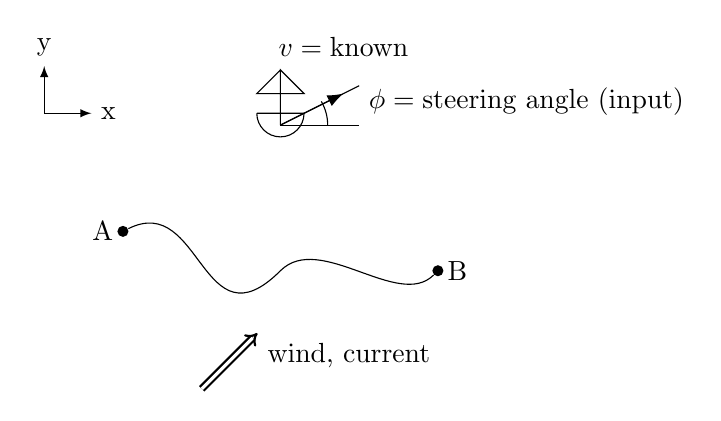
\begin{tikzpicture}
    \draw [->] (-3,0) -- ++(0.6,0) node [right] {x};
    \draw [->] (-3,0) -- ++(0,0.6) node [above] {y};

    \draw (-0.3,0) -- ++(0.6,0) arc (0:-180:0.3);
    \draw (0,-0.15) coordinate (a) -- ++(0,0.7) -- ++(0.3,-0.3) -- ++(-0.6,0) -- ++(0.3,0.3);
    \draw (a) -- ++(1,0) coordinate(b);
    \draw (a) -- ++(1,0.5) coordinate (c);
    \draw [-{Latex[scale=1.2]}] (a) -- ($(a)!0.8!(c)$) node [above,yshift=10pt] {$v={}$known};
    \coordinate (d) at ($(a)!0.6!(b)$);
    \draw let \p1 = ($(d)-(a)$) in (d) arc (0:30:\x1);
    \node [above right] at (b) {$\phi={}$steering angle (input)};

    \node [dot] (A) at (-2,-1.5) {};
    \node [left] at (A) {A};
    \node [dot] (B) at (2,-2) {};
    \node [right] at (B) {B};
    \draw (A) .. controls ++(1,0.5) and ++(-1,-1) .. ++(2,-0.5) .. controls ++(0.5,0.5) and ++(-0.5,-0.5) .. (B);
    \draw [double equal sign distance,-Implies,thick] (-1,-3.5) -- ++(45:1) node [below right] {wind, current};
  \end{tikzpicture}
\end{center}
The dynamics are
\begin{gather}
  \begin{aligned}
    \dot x &= v\cos\phi + c_1(x,y) \\
    \dot y &= v\sin\phi + c_2(x,y)
  \end{aligned}
  \qquad
  \lambda = \begin{bmatrix}
    \lambda_x \\ \lambda_y
  \end{bmatrix} 
\end{gather}
For minimum time, $L=1$.
\begin{align}
  H &= 1 + \lambda_x(v\cos\phi + c_1) + \lambda_y(v\sin\phi + c_2) \\
  0 &= \pder{H}{\phi} = -v \lambda_x \sin\phi + v \lambda_y \cos\phi \\
  \phi &= \tan^{-1} \left(\frac{\lambda_y}{\lambda_x}\right)
\end{align}
Since this is a conservative system and $\partial\Psi/\partial T=0$, then $H(t)=H(T)=0$.
\begin{align}
  -1 &= \lambda_x(v\cos\phi + c_1) + \lambda_y(v\sin\phi + c_2) \\
  \lambda_x &= - \frac{\cos\phi}{v + c_1\cos\phi + c_2\sin\phi} \\
  \lambda_y &= - \frac{\sin\phi}{v + c_1\cos\phi + c_2\sin\phi} \\
  \dot\lambda &= -\pder{H\trans}{x} \\
  \dot\lambda_x &= -\lambda_x\pder{c_1}{x} - \lambda_y\pder{c_2}{x} \\
  \dot\lambda_y &= -\lambda_x\pder{c_1}{y} - \lambda_y\pder{c_2}{y} \\
  \dot\phi &= \sin^2\phi \pder{c_2}{x} + \sin\phi \cos\phi \left(\pder{c_1}{x} - \pder{c_2}{y}\right) - \cos^2\phi \pder{c_1}{y}
\end{align}
This is an ODE that completely determines $\phi$ if we just had $\phi_0$.

% 2017/03/07
\paragraph{Example} We want to drive a car and stop at a stop sign as quickly as possible. Assume that the stop sign is at the origin, and our control is the acceleration ($\ddot x=u$).
\begin{align}
  & \min_{u,T} \int_0^T \!\dif t \\
  & \text{s.t. } \begin{dcases}
    \dot x_1 = x_2, & x(0) = x_0 \\
    \dot x_2 = u, & x(T) = 0
  \end{dcases}
\end{align}
Recall the transversality condition:
\begin{gather}
  \left. H + \pder{\Psi}{T} \right|_{t=T} = 0.
\end{gather}
For minimum-time problems, $L=1$ and $\Psi=0$, so $\lambda\trans f|_{t=T} = -1$.
\begin{gather}
  H = 1 + \lambda_1 x_2 + \lambda_2 u \\
  \lambda_1(T) \underbrace{x_2(T)}_{\mathclap{=0 \text{ (rest)}}} + \lambda_2(T) u(T) = -1 \\
  \boxed{\lambda_2(T) u(T) = -1} \\
  \pder{H}{u} = \boxed{ \lambda_2 = 0 },
\end{gather}
i.e.\ $0\cdot u(T) = -1$!? This problem is ill-posed; we need to go infinitely fast\dots

\begin{description}
\item[Idea 1:] Constrain $u$. We don't know how to do this.
\item[Idea 2:] Pay for gas. This is a design choice.
\end{description}

For the second idea,
\begin{align}
  & \min_{u,T} \int_0^T \! \frac{1}{2} u^2(t) \dif t \\
  & \text{s.t. } \begin{dcases}
    \dot x_1 = x_2, & x(0) = x_0 \\
    \dot x_2 = u, & x(T) = 0
  \end{dcases}
\end{align}
\begin{gather}
  H = \frac{1}{2} u^2 + \lambda_1 x_2 + \lambda_2 u \\
  \frac{1}{2} u^2(T) + \lambda_1(T) x_2(T) + \lambda_2(T) u(T) = 0 \\
  \boxed{ \frac{1}{2} u^2(T) + \lambda_2(T) u(T) = 0 } \\
  \pder{H}{u} = u + \lambda_2 = 0 \Longrightarrow u = -\lambda_2 \\
  \frac{1}{2} \lambda_2^2(T) - \lambda_2^2(T) = 0 \\
  \boxed{\lambda_2(T) = 0} \displaybreak \\
  \dot\lambda_1 = -\pder{H}{x_1} = 0 \Longrightarrow \lambda_1 = c \\
  \dot\lambda_2 = -\pder{H}{x_2} = -\lambda_1 \Longrightarrow \lambda_2 = -ct + d \\
  \lambda_2(T) = -cT + d = 0 \Longrightarrow T = \frac{d}{c} \\
  \dot x_2 = u = -\lambda_2 = ct - d \\
  x_2 = c \frac{t^2}{2} - dt + x_{2,0} \\
  \dot x_1 = x_2 \Longrightarrow x_1 = c \frac{t^3}{6} - d \frac{t^2}{2} + x_{2,0} t + x_{1,0} \\
  \begin{dcases}
    x_1(T) = c\frac{T^3}{6} - d \frac{T^2}{2} + x_{2,0} T + x_{1,0} = 0 \\
    x_2(T) = c\frac{T^2}{2} - dT + x_{2,0} = 0 \\
    T = \frac{d}{c}
  \end{dcases} \\
  \Longrightarrow \begin{dcases}
    c = -\frac{2}{3} \frac{x_{2,0}^2}{x_{1,0}} \\
    d = \sqrt{-\frac{4}{3} \frac{x_{2,0}^3}{x_{1,0}}} \\
    T = \frac{d}{c} \\
    u = ct - d
  \end{dcases}
\end{gather}

Fine, but we really want to get there as quickly as possible! We have to constrain $u$, e.g.\ $u(t)\in[-1,1]$, $\forall t\in[0,T]$. How do we deal with the constraints on $u$?

\section{Hamilton's Minor ``Mistake''}

\begin{align}
  \min_{u\in\mathcal{U}_{\text{constr.}}} {} & \int_0^T L(x,u,t)\dif t + \Psi(x(T)) \\
  \text{s.t. } & \dot x = f(x,u,t) \\
            & x(0) = x_0 \\
            & ( u(t) \in U )
\end{align}
Augment the cost:
\begin{gather}
  \tilde J(u) = \int_0^T \Big( H(x,u,t,\lambda) - \lambda\trans \dot x \Big) \dif t + \Psi(x(T))
\end{gather}
Vary $u\mapsto u+\varepsilon v$ s.t.\ $u+\varepsilon v\in\mathcal U_{\text{constr.}} \Rightarrow x\mapsto x +\varepsilon\eta+o(\varepsilon)$:
\begin{gather}
\begin{align}
  \tilde J(u+\varepsilon v) &= \int_0^T \Big( H(x+\varepsilon\eta,u+\varepsilon v,t,\lambda) - \lambda\trans\dot x - \lambda\trans\varepsilon\dot\eta \Big) \dif t + \Psi(x(T) + \varepsilon\eta(T)) + o(\varepsilon) \\
  \shortintertext{Instead of computing $\delta\tilde J(u;v)$, let's check $\Delta\tilde J=\tilde J(u+\varepsilon v)-\tilde J(u)$. If $\Delta\tilde J\ge 0$ $\forall v$ s.t.\ $u+\varepsilon v\in\mathcal U_{\text{constr.}}$ for $\varepsilon$ small enough, then $u$ is a local minimum!}
  \Delta\tilde J &= \int_0^T \Big[ H(x+\varepsilon\eta,u+\varepsilon v,t,\lambda) - H(x,u,t,\lambda) - \lambda\trans(\dot x + \varepsilon\dot\eta - \dot x) \Big] \dif t \\
                            & \qquad + \Psi(x(T)+\varepsilon\eta(T)) - \Psi(x(T)) + o(\varepsilon) \\
  \shortintertext{Only Taylor expanding w.r.t.\ $x$:}
  \Delta\tilde J &= \int_0^T \left[\varepsilon\pder{H}{x}(x,u,t,\lambda)\eta - \varepsilon\lambda\trans\dot\eta \right] \dif t + \int_0^T \big[ H(x,u+\varepsilon v,t,\lambda) - H(x,u,t,\lambda) \big] \dif t \\
                            & \qquad + \varepsilon\pder{\Psi}{x}(x(T))\eta(T) + o(\varepsilon) \\
                            &= \varepsilon \int_0^T \left( \pder{H}{x} + \dot\lambda\trans \right) \eta\dif t + \varepsilon\lambda\trans(0)\eta(0) - \varepsilon\lambda\trans(T)\eta(T) + \varepsilon\pder{\Psi}{x}(x(T))\eta(T) \\
                            & \qquad + \int_0^T \big[ H(x,u+\varepsilon v,t,\lambda) - H(x,u,t,\lambda) \big]\dif t + o(\varepsilon) \\
  \shortintertext{With $\dot\lambda=-\partial H\trans/\partial x$ and $\lambda(T)=\partial\Psi(x(T))/\partial x$,}
  \Delta\tilde J &= \int_0^T \big[ H(x,u+\varepsilon v,t,\lambda) - H(x,u,t,\lambda) \big]\dif t + o(\varepsilon)
\end{align} \\
  \shortintertext{Here, Hamilton did Taylor's expansion and set $\partial H/\partial u=0$. Instead, Pontryagin desired $\Delta\tilde J\ge 0$ $\forall v|u+\varepsilon v\in\mathcal U_{\text{constr.}}$, $\varepsilon$ small enough, i.e.\ we need}
                            H(x,u^*+\varepsilon v,t,\lambda) \ge H(x,u^*,t,\lambda) \\
  \shortintertext{$\forall t\in[0,t]$, $\forall v|u+\varepsilon v\in\mathcal U_{\text{constr.}}$, $\varepsilon$ small enough. That is, we need}
  u^* = \arg\min_u H(x,u,t,\lambda)
\end{gather}
In summary,
\begin{align}
  &\text{Hamilton: } \pder{H}{u} = 0 \\
  &\text{Pontryagin: } \min_u H
\end{align}

\begin{oframed}
\begin{thm}[Pontryagin's Maximum Principle (PMP)]
  Consider the problem:
  \begin{align}
    \min_{u,T} {} & \int_0^T\! L(x,u,t)\dif t + \Psi(x(T),T) \\
    \text{s.t. } & \begin{aligned}[t]
      & \dot x = f(x,u,t) \\
      & u(t)\in U(x,t), && \forall t\in[0,T] \\
      & x_i(0) = x_{i0}, && i\in\mathcal I \\
      & x_j(T) = x_{jT}, && j\in\mathcal T
    \end{aligned} 
  \end{align}
  The necessary condition for optimality is
  \begin{align}
    & H = L + \lambda\trans f \\
    & \dot\lambda = -\pder{H\trans}{x} \\
    & \lambda_j(0) = 0, \quad j\not\in\mathcal I \\
    & \lambda_i(T) = \pder{\Psi}{x_i}(x(T)), \quad i\not\in\mathcal T \\
    & \left. H + \pder{\Psi}{T} \right|_{t=T} = 0 \\
    & u^*(x,t,\lambda) = \arg\min_{\mathclap{u\in U(x,t)}} \; H(x,u,t,\lambda)
  \end{align}
\end{thm}
\end{oframed}

% 2017/03/09
We have two paths to solve optimality problems: we always start with the Hamiltonian, find the costate dynamics and boundary conditions, and apply the transversality condition; then, we can either apply calculus of variations (COV) or Pontryagin's Maximum Principle (PMP). COV only works for unconstrained problems, while with PMP we can deal with constraints.

\section{Bang-Bang Control}
Return to the car problem:
\begin{align}
  & \min_{u,T} \int_0^T \!\dif t \\
  & \text{s.t. } \adjustbox{valign=t}{$
    \begin{dcases}
      \begin{aligned}
        \dot x_1 &= x_2, & x_1(0) &= x_{1,0}, & x_1(T) &= 0 \\
        \dot x_2 &= u, & x_2(0) &= x_{2,0}, & x_2(T) &= 0 \\
      \end{aligned} \\
      u(t)\in[-1,1] \quad \forall t\in[0,T]
    \end{dcases}
  $}
\end{align}
How do we minimize $H$ w.r.t.\ $u$?
\begin{align}
  H &= 1 + \lambda_1 x_2 + \lambda_2 u
\end{align}
Clearly, we minimize $H$ by letting
\begin{gather}
  u = \begin{dcases}
    -1, & \lambda_2 > 0 \\
    +1, & \lambda_2 < 0 \\
    \text{??}, & \lambda_2 = 0
  \end{dcases}
  = -\sign(\lambda_2)
\end{gather}
Therefore, the optimal $u$ switches between $-1$ and $+1$ (bang-bang control).
\begin{gather}
  \dot \lambda_1 = -\pder{H}{x_1} = 0 \Longrightarrow \lambda_1 = c \\
  \dot \lambda_2 = -\pder{H}{x_2} = -\lambda_1 \Longrightarrow \lambda_2 = -ct + d
\end{gather}
Notice that $\lambda_2(t)$ is a line, so it has at most one sign change. Thus, $u$ also changes sign (from $\pm1$ to $\mp1$) at most one time.

\begin{center}
  \begin{tikzpicture}
    \def\T{4.25}
    
    \draw [thick,->] (-1,0) -- (5,0) node [right] {$t$};
    \draw [thick,->] (0,-2.5) -- (0,2.5) node [above] {$\lambda_2$};
    \draw [thick] (\T,0.2) -- (\T,-0.2) node [below] {$T$};

    \draw (0,1) -- (\T,2.25) node [right] {0 sign changes};
    \draw (0,-1) -- (\T,1) node [right] {1 sign change};
    \draw (0,2) -- (\T,-2) node [right] {1 sign change};
    \draw (0,-2.25) -- (\T,-1) node [right] {0 sign changes};
    \draw [line width=2.5pt] (0,0) node [pin=above left:{$\lambda_2=0$}] {} -- (\T,0);
  \end{tikzpicture}
\end{center}

Let's solve this for all $x_0$!
\begin{enumerate}[label=\roman*)]
\item Assume $\lambda_2>0$ $\forall t\in[0,T]$, $\therefore u = -1 \quad \forall t\in[0,T]$
  \begin{align}
    \dot x_2 &= -1 \Longrightarrow x_2 = -t + k_1 \\
    x_2(T) &= 0 = -T + k_1 \Longrightarrow k_1 = T \\
    x_2(t) &= T - t \Longrightarrow x_2 > 0,\ t\in[0,T) \\
    \dot x_1 &= x_2 = T - t \Longrightarrow x_1 = -\frac{t^2}{2} + Tt + k_2 \\
    x_1(T) &= 0 = -\frac{T^2}{2} + T^2 + k_2 \Longrightarrow k_2 = -\frac{T^2}{2} \\
    x_1(t) &= -\frac{t^2}{2} + Tt - \frac{T^2}{2} = -\frac{(T-t)^2}{2} \quad (<0,\ t\in[0,T)) \\
           &= -\frac{x_2^2(t)}{2}
  \end{align}
  Let's consider the curve
  \begin{gather}
    \begin{bmatrix}
      -x_2^2/2 \\ x_2
    \end{bmatrix}
  \end{gather}
  for $x_2\ge 0$. If $x_0$ lies on this curve, use $u=-1$ and drive to the origin.

\item Assume $u=+1 \quad \forall t\in[0,T]$
  \begin{align}
    x_2 &= t - T \quad (\le 0 \text{ on } [0,T]) \\
    x_1 &= \frac{x_2^2}{2} \quad (\ge 0)
  \end{align}
  For this curve, use $u=+1$.
\end{enumerate}

\begin{center}
  \begin{tikzpicture}
    \draw [thick,->] (-3,0) -- (3,0) node [right] {$x_1$};
    \draw [thick,->] (0,-3) -- (0,3) node [above] {$x_2$};
    \node [dot] at (0,0) {};

    \draw [rotate=90] (0,0) parabola (3,3) node [above] {$[-x_2^2/2,\ x_2]\trans,\ x_2\ge 0$};
    \draw [very thin,-<,>={Straight Barb[scale=3,line width=1pt]},rotate=90] (0,0) parabola (2.12,1.5);
    \node [pin={[pin distance=1cm]30:{curve if $u=-1$ $\forall t$}}] at (-0.8,1.5) {};

    \draw [rotate=-90] (0,0) parabola (3,3) node [below] {$[x_2^2/2,\ x_2]\trans,\ x_2\le 0$};
    \draw [very thin,-<,>={Straight Barb[scale=3,line width=1pt]},rotate=-90] (0,0) parabola (2.12,1.5);
    \node [pin={[pin distance=1cm]30:{curve if $u=+1$ $\forall t$}}] at (0.8,-1.5) {};
  \end{tikzpicture}
\end{center}

What happens when we do not start on the curves? We start with a certain $u$ depending on $x_0$ and perform a single switch of $u$ when we encounter one of the initial curves that travel to the origin. Note that for the case $\lambda_2=0 \forall t$, we start at the stop sign at rest, so the control does not matter.

\begin{center}
  \begin{tikzpicture}
    \draw [thick,->] (-3,0) -- (3,0) node [right] {$x_1$};
    \draw [thick,->] (0,-3) -- (0,3) node [above] {$x_2$};
    \node [dot] at (0,0) {};
    \draw [rotate=90,ultra thick] (0,0) parabola (3,3) node [above] {$u=-1$};
    \draw [very thin,-<,>={Straight Barb[scale=3,line width=1pt]},rotate=90] (0,0) parabola (2.12,1.5);
    \draw [rotate=-90,ultra thick] (0,0) parabola (3,3) node [below] {$u=+1$};
    \draw [very thin,-<,>={Straight Barb[scale=3,line width=1pt]},rotate=-90] (0,0) parabola (2.12,1.5);

    \draw [rotate=90,xshift=-1cm,yshift=1cm] (-3,3) node [below] {off to $\infty$} parabola bend (0,0) (3,3) node [above left] {$u=-1$};
    \draw [very thin,-<,>={Straight Barb[scale=3,line width=1pt]},rotate=90,xshift=-1cm,yshift=1cm] (0,0) parabola (2.12,1.5);
    \draw [very thin,->,>={Straight Barb[scale=3,line width=1pt]},rotate=90,xshift=-1cm,yshift=1cm] (0,0) parabola (-2.12,1.5);

    \draw [rotate=90,xshift=-0.5cm,yshift=0.5cm] (0,0) parabola (3,3);
    \draw [very thin,-<,>={Straight Barb[scale=3,line width=1pt]},rotate=90,xshift=-0.5cm,yshift=0.5cm] (0,0) parabola (2.12,1.5);
    \draw [rotate=90,xshift=-1.5cm,yshift=1.5cm] (0,0) parabola (3,3);
    \draw [very thin,-<,>={Straight Barb[scale=3,line width=1pt]},rotate=90,xshift=-1.5cm,yshift=1.5cm] (0,0) parabola (2.12,1.5);

    \draw [rotate=90,xshift=0.5cm,yshift=-0.75cm] (0,0) parabola (3,3);
    \draw [very thin,-<,>={Straight Barb[scale=3,line width=1pt]},rotate=90,xshift=0.5cm,yshift=-0.75cm] (0,0) parabola (2.12,1.5);
    \draw [rotate=90,xshift=0.5cm,yshift=-3cm] (0,0) parabola (3,3) node [right,xshift=1cm] {$u=-1$};
    \draw [very thin,-<,>={Straight Barb[scale=3,line width=1pt]},rotate=90,xshift=0.5cm,yshift=-3cm] (0,0) parabola (2.12,1.5);

    \node [dot] at (0.72,-1.46) {};
    \clip (-3,3.5) rectangle (3,-1.46);
    \draw [rotate=90,xshift=0.5cm,yshift=-2cm] (-3,3) parabola bend (0,0) (3,3);
    \draw [very thin,-<,>={Straight Barb[scale=3,line width=1pt]},rotate=90,xshift=0.5cm,yshift=-2cm] (0,0) parabola (2.12,1.5);
  \end{tikzpicture}
\end{center}

\clearpage
The optimal solution is given by the following \emph{switching curve}.
\begin{center}
  \begin{tikzpicture}
    \draw [thick,->] (-3,0) -- (3,0) node [right] {$x_1$};
    \draw [thick,->] (0,-3) -- (0,3) node [above] {$x_2$};
    \node [dot] at (0,0) {};

    \draw [rotate=90] (0,0) parabola (3,3) node [above] {$[-x_2^2/2,\ x_2]\trans,\ x_2\ge 0$};
    \draw [very thin,-<,>={Straight Barb[scale=3,line width=1pt]},rotate=90] (0,0) parabola (2.12,1.5) node [above right] {$u=-1$};

    \draw [rotate=-90] (0,0) parabola (3,3) node [below] {$[x_2^2/2,\ x_2]\trans,\ x_2\le 0$};
    \draw [very thin,-<,>={Straight Barb[scale=3,line width=1pt]},rotate=-90] (0,0) parabola (2.12,1.5) node [below left] {$u=+1$};

    \node [right] at (1,1) {$\boxed{u=-1}$};
    \node [left] at (-1,-1) {$\boxed{u=+1}$};
  \end{tikzpicture}
\end{center}

\begin{description}
\item[Note 1:] Bang-bang control typically involves
  \begin{enumerate}[label=\alph*),nolistsep]
  \item finding the number of switches
  \item find the switching surfaces
  \end{enumerate}
\item[Note 2:] This is a feedback law! ($u$ depends on $x$!!)
\end{description}

\subsection{Linear Systems (scalar input)}
\begin{align}
  \min_{u,T} {} & \int_0^T \!\dif t \\
  \text{s.t. } & \dot x = Ax + Bu \\
                & x(0) = x_0, \quad x(T) = 0 \\
                & u\in[-1,1] \\
  H &= 1 + \lambda\trans (Ax + Bu) \\
  u &= -\sign (\lambda\trans B) \quad \text{(bang-bang)}
\end{align}
Aside\dots
\begin{align}
  \dot x &= f(x) + g(x) u \quad \text{(control affine)} \\
  H &= 1 + \lambda\trans f + \lambda\trans g u \\
  u &= -\sign (\lambda\trans g(x)) \quad \text{(bang-bang)}
\end{align}
Back to linear\dots
\begin{align}
  \dot\lambda &= -\pder{H\trans}{x} = -A\trans\lambda \\
  \lambda(t) &= e^{-A\trans t} \lambda_0 \\
  u(t) &= -\sign\left( \lambda_0\trans e^{-At} B \right)
\end{align}
How do we find $\lambda_0$?
\begin{align}
  \dot x &= Ax + Bu, \quad x(0) = x_0 \\
  x(T) &= e^{AT} x_0 + \int_0^T e^{A(T-\tau)} Bu(\tau) \dif\tau \\
  x(T) &= 0 = e^{AT}x_0 - \int_0^T e^{A(T-t)} B \sign \left( \lambda_0\trans e^{-At} B \right) \dif t \label{eq:linsys_xT}
\end{align}
\emph{Problem 1:} Given $x_0$, figure out $\lambda_0$ from \eqref{eq:linsys_xT}. Then, $u=-\sign\left( \lambda_0\trans e^{-At} B \right)$. This has to be done numerically in general (not super simple\dots).

\bigskip
\noindent
\emph{Problem 2:} Find all $x_0$s from which it takes the same amount of time to get to $x(T)=0$.
\begin{align}
  e^{At}x_0 &= \int_0^T e^{A(T-t)} B \sign \left( \lambda_0\trans e^{-At} B \right) \dif t \\
  x_0 &= \int_0^T e^{-At} B \sign \left( \lambda_0\trans e^{-At} B \right) \dif t \label{eq:linsys_x0}
\end{align}
Fix $T$. By varying $\lambda_0$, we will get the $x_0$s that take time $T$ to go to $x(T)=0$ optimally.
\begin{center}
  \begin{tikzpicture}
    \node [dot] at (0,0) {};
    \node [below,yshift=-1pt] at (0,0) {$O$};
    \draw [decorate,decoration={snake,segment length=1cm}] (0,0) circle (2);
    \path (0,0) -- ++(40:2.2) coordinate (a);
    \draw [{Straight Barb[scale=2]}-,thick] (a) to[out=40,in=180] ++(20:1.5) node [right,align=left] {contours of \\ constant \\ time-to-go};

    \path (0,0) -- ++(-20:2.2) coordinate (b);
    \draw [{Straight Barb[scale=2]}-,thick] (b) to[out=-30,in=180] ++(-20:1.5) node [right] {$(T,\lambda_0)\Rightarrow u$};
  \end{tikzpicture}
\end{center}
So by solving problem 2, we find $\lambda_0$ associated with all $x_0$, i.e.\ we have ``solved'' problem 1 as well.

% 2017/03/14
\section{Integral Constraints (Isoperimetric)}
Recall PMP is
\begin{gather}
  \min_{u\in U(x,t)} H(x,u,\lambda,t)
\end{gather}
We have see $U=[-1,1]$ in the context of bang-bang control. Now, we consider integral constraints of the form
\begin{gather}
  C = \int_0^T \! N(x,u,t)\dif t \quad (\in \R^p)
\end{gather}
Let $x=[x_1,\dots,x_n]\trans \in\R^n$. Introduce $p$ new states $\hat x=[x_{n+1},\dots,x_{n+p}]\trans$, where
\begin{gather}
  \hat x(t) = \int_0^t\! N(x(\tau),u(\tau),\tau)\dif\tau
\end{gather}
and $\dot{\hat x}(t)=N(x,u,t)$. Its boundary conditions are $\hat x(0)=0$ and $\hat x(T)=C$. The Hamiltonian is
\begin{gather}
  H(x,\hat{x},u,t,\lambda) = L(x,u,t) + \lambda\trans f(x,u,t) + \widehat{\lambda}\trans N(x,u,t) \\
  \begin{aligned}
    \dot\lambda &= -\pder{H\trans}{x} = -\pder{L\trans}{x} - \pder{f\trans}{x}\lambda - \pder{N\trans}{x}\widehat\lambda \\
    \dot{\widehat\lambda} &= -\pder{H\trans}{\hat x} = 0 \Longrightarrow \widehat\lambda \text{ is constant}
  \end{aligned}
\end{gather}
Moreover, this is now an unconstrained problem, i.e.
\begin{gather}
  \pder{H}{u} = \pder{L}{u} + \lambda\trans\pder{f}{u} + \widehat{\lambda}\trans \pder{N}{u} = 0
\end{gather}

Going back to the car problem of stopping at the origin, suppose we want to use up exactly the ``energy''
\begin{gather}
  E = \int_0^T\! u^2(t)\dif t.
\end{gather}
\emph{If possible, it is better to transform an inequality constraint to an equality constraint.}
\begin{align}
  \min_{u,T} {} & \int_0^T \dif t \\
  \text{s.t. } & \adjustbox{valign=t}{$
                 \begin{dcases}
                   \begin{aligned}
                     \dot x_1 &= x_2, & x_1(0) &= x_{10}, & x_1(T) &= 0 \\
                     \dot x_2 &= u, & x_2(0) &= x_{20}, & x_2(T) &= 0 \\
                     \dot x_3 &= u^2, & x_3(0) &= 0, & x_3(T) &= E
                   \end{aligned}
                 \end{dcases}$}
\end{align}
As we have seen, without the energy constraint this is an ill-posed problem.
\allowdisplaybreaks
\begin{align}
  H &= 1 + \lambda_1 x_2 + \lambda_2 u + \lambda_3 u^2 \\
  \lambda_3 &= \text{constant} \\
  \dot\lambda_1 &= -\pder{H}{x_1} = 0 \Longrightarrow \lambda_1 = c \\
  \dot\lambda_2 &= -\pder{H}{x_2} = -\lambda_1 \Longrightarrow \lambda_2 = -ct + d \\
  \pder{H}{u} &= \lambda_2 + 2\lambda_3 u = 0 \\
  \Rightarrow u &= -\frac{\lambda_2}{2\lambda_3} = \frac{c}{2\lambda_3} t - \frac{d}{2\lambda_3} \quad \text{(linear in time)} \\
  \dot x_2 &= u \Longrightarrow x_2 = \frac{c}{4\lambda_3} t^2 - \frac{d}{2\lambda_3} t + x_{20} \\
  \dot x_1 &= x_2 \Longrightarrow x_1 = \frac{c}{12\lambda_3} t^3 - \frac{d}{4\lambda_3} t^2 + x_{20} t + x_{10} \\
  \dot x_3 &= u^2 \Longrightarrow x_3 = \frac{c^2}{12\lambda_3^2} t^3 + \frac{d^2}{4\lambda_3^2} t - \frac{cd}{4\lambda_3^2} t^2 \\
    & \left. H + \pder{\Psi}{T} \right|_T = 0 \\
    & 1 + \lambda_1 x_2 + \lambda_2 u + \lambda_3 u^2 + 0 \Big|_T = 0 \\
    & 1 + (d-cT) \left(\frac{c}{2\lambda_3} T - \frac{d}{2\lambda_3}\right) + \lambda_3 \left(\frac{c}{2\lambda_3} T - \frac{d}{2\lambda_3}\right) = 0 \\
  \shortintertext{The boundary conditions ($x_1(T)=0$, $x_2(T)=0$, $x_3(T)=E$) and the transversality condition give four equations for four unknowns.}
  & \begin{dcases}
    T = \left(\frac{3}{E}\right)^{1/3} \\
    c = -\frac{2}{3} T \\
    d = -\frac{T^2}{3} \\
    \lambda_3 = \frac{T^4}{18}
  \end{dcases} \quad \Longrightarrow u = \dots
\end{align}
\allowdisplaybreaks[0]

\paragraph{Dido's Problem}
Given a strip of oxhide, enclose the most area along the Mediterranean Sea. This region has a fixed width and is bounded to the south by the $\ell$ axis (the sea). Historically, this became the city Carthage.

\begin{center}
  \begin{tikzpicture}
    \draw [->,thick] (-3,0) -- (3,0) node [right] {$\ell$};
    \draw [->,thick] (0,-0.5) -- (0,3) node [above] {$y$};
    \foreach \x/\a in {-2.5/-a,2.5/a}
    \draw [thick] (\x,0.2) -- (\x,-0.2) node [below] {$\a$};

    \draw (-2.5,0) .. controls (-2,1.5) and (-1.5,0) .. (-0.5,1.5);
    \draw (2.5,0) .. controls (2,1.5) and (1.5,0) .. (1,1.5);
    \draw (1,1.5) parabola [bend pos=0.3] bend +(0,0.75) (-0.5,1.5);

    \node [pin=above right:{rope of length $P$}] at (1,1.5) {};
    \draw [-{Straight Barb[scale=2]},thick] (-2.2,0.6) -- ++(50:2);
    \draw [thick] (-2.2,0.6) -- ++(1.5,0);
    \draw (-1.2,0.6) arc (0:50:1);
    \node [pin=above left:{control variable}] at (-1.1,1.3) {$\theta$};
  \end{tikzpicture}
\end{center}
The area of this region is
\begin{gather}
  \int_{-a}^a \! y \dif\ell.
\end{gather}
The dynamics are
\begin{gather}
  \frac{\dif y}{\dif\ell} = \tan\theta.
\end{gather}
The constraint is
\begin{gather}
  P = \int_{-a}^a \! \frac{1}{\cos\theta} \dif\ell.
\end{gather}
The problem becomes
\begin{align}
  \min_\theta {} & -\int_{-a}^a \! y(\ell) \dif\ell \\
  \text{s.t. } & \frac{\dif y}{\dif\ell} = \tan\theta, \quad y(-a)=0,\quad y(a)=0 \\
                 & \frac{\dif\hat y}{\dif\ell} = \frac{1}{\cos\theta}, \quad \hat y(-a)=0,\quad \hat y(a)=P
\end{align}
\begin{align}
  H &= -y + \lambda\tan\theta + \widehat\theta \frac{1}{\cos\theta} \\
  \widehat\lambda &= \text{constant} \\
  \frac{\dif\lambda}{\dif\ell} &= -\pder{H}{y} = 1 \Longrightarrow \lambda(\ell) = \ell + c \\
  \pder{H}{\theta} &= 0 = \lambda (1 + \tan^2\theta) + \widehat\lambda\, \frac{\tan\theta}{\cos\theta} \\
  \sin\theta(\ell) &= -\frac{\ell + c}{\widehat\lambda}
\end{align}
Let $\sin\alpha/\alpha = 2a/P$. The optimal shape is a circular arc centered at $\ell=0$ and
\begin{gather}
  y = - \frac{P\cos\alpha}{2\alpha},
\end{gather}
with radius $P/2\alpha$. (This produces the semi-circular city of Carthage!)
\begin{center}
  \begin{tikzpicture}
    \draw [->,thick] (-3,0) -- (3,0) node [right] {$\ell$};
    \draw [->,thick] (0,-4) -- (0,2) node [above] {$y$};
    \foreach \x/\a in {-2/-a,2/a}
    \draw [thick] (\x,-0.2) -- (\x,0.2) node [above,xshift=-2pt] {$\a$};

    \node [dot] at (0,-1) {};
    \draw [dashed] (0,-1) circle (veclen(2,1));
    \draw (2,0) arc (atan(1/2):180-atan(1/2):veclen(2,1));
  \end{tikzpicture}
\end{center}
\emph{Note that this formulation cannot handle $P>\pi a$. In reality, $a$ is also undefined and chosen so that the solution is exacty a semicircle with $P=\pi a$.}

The punchline is integral constraints are no big deal. What about other constraints?

\section{Control Constraints}
Suppose the control constraint is $u(t)\in U(t)$, e.g. $h(u,t)=0$ or $h(u,t)\le 0$.
\begin{align}
  \min_u {} & H(x,u,\lambda,t) \\
  \text{s.t. } & h(u,t) = 0
\end{align}
Introduce a Lagrange multiplier:
\begin{align}
  & \tilde H = H + \mu\trans h \\
  & \left. \begin{aligned}
    & \pder{\tilde H}{u} = 0 \\
    & h = 0
  \end{aligned} \right\} \Longrightarrow u^*(x,t,\lambda)
\end{align}
We still have
\begin{align}
  \dot\lambda &= -\pder{H\trans}{x} (x,t,\lambda,u^*(x,t,\lambda)) \\
  \dot x &= f(x,u,t) = f(x,u^*(x,t,\lambda),t) \\
              & \quad + \text{Boundary cond.\ on $x$ and $\lambda$}
\end{align}
The only change from the unconstrained control version is the method by which $u^*(x,t,\lambda)$ is found.

% 2017/03/16
\paragraph{Example} \mbox{}
\begin{align}
  \min_u {} & \frac12 \int_0^T u^2(t)\dif t + \frac12 \Vert x(T)\Vert^2 \\
  \text{s.t. } & \dot x=g(t) u, \quad g(t)\in\R^n \\
            & |u(t)| \le 1 \ \forall t \\
            & \Rightarrow \begin{dcases}
              u(t) - 1 \le 0 \\
              -u(t) - 1 \le 0
            \end{dcases}
\end{align}
\begin{align}
  H &= \frac12 u^2 + \lambda\trans gu \\
  \widetilde H &= \frac12 u^2 + \lambda\trans gu + \mu_1(u-1) + \mu_2(-u-1) \\
  \dot\lambda &= -\pder{\widetilde H\trans}{x} = 0 \Longrightarrow \lambda=\text{const} \\
  \lambda(T) &= \pder{\Psi\trans}{x} = x(T) \Longrightarrow \lambda(t) = x(T) \ \forall t \\
               \shortintertext{Now, let's find $u$ by minimizing $H$. Assume $|u|<1$ (no constraints active), so $\mu_1=\mu_2=0$. Then,}
  \pder{\widetilde H}{u} &= u + \lambda\trans g = 0 \Longrightarrow u(t) = -x\trans(T) g(t), \\
  \shortintertext{as long as $|x\trans(T)g(t)|<1$. Assume $u=-1$, so $\mu_1=0$ and $\mu_2\ge0$. Then,}
  \pder{\widetilde H}{u} &= u + \lambda\trans g - \mu_2 = 0 \\
    & x\trans(T) g(t) = \mu_2 + 1 \ge 1 \\
  \shortintertext{We get a similar results assuming $u=1$. The optimal control law is}
  u(t) &= \begin{dcases}
    -x\trans(T)g(t), & |x\trans(T)g(t)| < 1 \\
    -1, & x\trans(T)g(t) \ge 1 \\
    +1, & x\trans(T)g(t) \le -1
  \end{dcases} \\
  u(t) &= -\mathop\text{Sat}(x\trans(T)g(t)) \\
  \shortintertext{where}
  \mathop\text{Sat}(\xi) &= \begin{dcases}
    \xi, & |\xi| \le 1 \\
    \sign(\xi), & \text{otherwise}
  \end{dcases}
\end{align}
Problem: we don't know $x(T)$! We have to solve this numerically through
\begin{gather}
  x(t) = x(0) + \int_0^t \dot x(\tau)\dif\tau \\
  x(T) = x_0 - \int_0^T g(t) \mathop\text{Sat}\big(x\trans(T)g(t)\big) \dif t
\end{gather}

\paragraph{Example} \mbox{}
\begin{align}
  \min_u {} & \int_0^T L(x,u,t)\dif t + \Psi(x(T)) \\
  \text{s.t. } & \dot x = f(x,u,t), \quad x(0)=x_0 \\
            & h(x,u,t) = 0\ \forall t
\end{align}
\begin{align}
  \widetilde H &= L + \lambda\trans f + \mu\trans h \\
  \dot\lambda &= -\pder{\widetilde H\trans}{x} = -\pder{L\trans}{x} - \pder{f\trans}{x}\lambda - \pder{h\trans}{x}\mu \\
  \lambda(T) &= \pder{\Psi\trans}{x}(x(T)) \\
  \pder{\widetilde H}{u} &= 0 \\
  h &= 0
\end{align}

\paragraph{Example} \mbox{}
\begin{align}
  \min_u {} & \int_0^T L(x,u,t)\dif t + \Psi(x(T)) \\
  \text{s.t. } & \dot x = f(x,u), \quad x(0)=x_0 \\
            & h(x) = 0
\end{align}
Problem: We need a constraint involving $u$. First, we need $h(x_0)=0$; otherwise we have no chance. Then, if
\begin{gather}
  \frac{\dif}{\dif t} h(x(t)) = \pder{h}{x} \dot x = \pder{h}{x} f(x,u) = 0,
\end{gather}
we have $h(x(t))=0$ $\forall t$. This derivative is the Lie derivative of $h$ along $f$ ($L_f h=(\partial h/\partial x)f$).
\begin{gather}
  \widetilde H = L + \lambda\trans f + \mu\trans \pder{h}{x} f
\end{gather}
Problem: $(\partial h/\partial x)f$ is not guaranteed to have $u$ in it, e.g.
\begin{gather}
  h = x_1, \quad f=\begin{bmatrix}
    17 x_2 \\ \sin(x_1) u
  \end{bmatrix} \\
  \pder{h}{x} f = \begin{bmatrix}
    1 & 0
  \end{bmatrix}
  \begin{bmatrix}
    17 x_2 \\ \sin(x_1) u
  \end{bmatrix}
  = 17 x_2
\end{gather}
So, we keep taking derivatives until $u$ shows up. (If $u$ never shows up, then the control has no effect on the state.)

\section{A Look Forward}
So far, we found $u(t)$ over the horizon $[0,T]$. This is, in general, not robust. We need to know $f$ exactly. We also need to know $x(0)$. What to do?

There are three paths forward:
\begin{enumerate}
\item If we're super lucky, we get $u(x,t)$ directly from PMP, like in the bang-bang example with switching surfaces.
\item Go from PMP to LQ (linear system, quadratic cost). This is used a lot.
\item Use Model-Predictive Control (MPC). In this, at time $t_c$ (current time), we are at state $x_c$. We solve an optimal control problem:
  \begin{align}
    \min_u {} & \int_{t_c}^{\mathrlap{t_c+\Delta T}} L(x,u,t)\dif t + \Psi(x(t_c+\Delta T)) \\
    \text{s.t. } & \dot x = f(x,u,t) \\
              & x(t_c) = x_c
  \end{align}
  where $\Delta T$ is the prediction horizon. This problem can be solved using PMP, producing $u(t)$, $t\in[t_c,t_c+\Delta T]$. Instead of using $u(t)$, only use $u(t_c)$ at time $t_c$. This control solution depends on $x_c$, so we really have a feedback law $u(x_c,t_c)$. (In practice, we use $u(x_c,t_c)$ over a small interval of length $\delta$.) Then, we resolve the optimal control problem.

  The features of MPC are
  \begin{enumerate}[nosep]
  \item Turns open-loop into closed-loop
  \item Used a lot
  \item Requires computation, but once a solution is found, it can be reused as initial conditions\dots
  \item Use with caution! A solution may be optimal over $[t_c,t_c+\Delta T]$ but it may still be bad (unstable) over $[t_c,\infty)$.
  \end{enumerate}
\end{enumerate}

%%% Local Variables:
%%% mode: latex
%%% TeX-master: "../notes"
%%% End:
\chapter{Linear-Quadratic Control}

% 2017/03/28
\section{Towards Global Optimal Control}
Consider a discrete-time system
\begin{gather}
  x_{k+1} = F(x_k,u_k),
\end{gather}
where $x_k$ is the state at time $k$ and $u_k$ is the input at time $k$.

Let $c(x_k,u_k)\in\R$ be the cost associated with doing $u_k$ at $x_k$.

Let $u=u_0,u_1,\dots,u_{N-1}$ and assume $x_0$ is given. The total cost over $N$ steps using $u$ is
\begin{gather}
  V_N^u(x_0) = \sum_{k=0}^{N-1} c(x_k,u_k) + \Theta(x_N),
\end{gather}
where $\Theta(x_N)$ is the terminal cost.

Assume we've found the \emph{globally} minimizing $u^*$. The best path over $N$ steps is represented by the figure below.
\begin{center}
  \begin{tikzpicture}
    \node [dot] (x0) at (0,0) {};
    \node [dot] (x1) at (1,0.2) {};
    \node [dot] (x2) at (2,0.3) {};
    \node [dot] (x3) at (3,1) {};
    \node [dot] (x4) at (4,-0.5) {};
    \node [dot] (x5) at (5,0.6) {};
    \node [dot] (xN) at (6,0.4) {};

    \node [below] at (x0) {$x_0$};
    \node [below] at (x1) {$x_1$};
    \node [below] at (x2) {$x_2$};
    \node [below] at (xN) {$x_N$};

    \draw [->] (x0) to[bend left] (x1);
    \draw [->] (x1) to[bend right] (x2);
    \draw [->] (x2) to[bend left] (x3);
    \draw [->] (x3) .. controls (3.8,1) and (3.2,-0.5) .. (x4);
    \draw [->] (x4) .. controls (4.5,-0.5) and (4.2,0.5) .. (x5);
    \draw [->] (x5) to[bend left] (xN);

    \draw [->,dashed] (x1) to[out=55,in=125] ($(xN)+(0,0.1)$);
  \end{tikzpicture}
\end{center}
Consider the dashed path. There is no way this path is better from $x_1$ to $x_N$ using $N-1$ steps. Therefore, the solid path from $x_1$ to $x_N$ is the best path over $N-1$ steps.

\clearpage
\begin{framed}
  \begin{defi}[Bellman's Principle of Optimality]
    Let $u^*$ be optimal, with corresponding state sequence $x^*$.
    \begin{align}
      V^*_N(x_0) &= \sum_{k=0}^{N-1} c(x_k^*,u_k^*) + \Theta(x_N^*) \\
      &= c(x_0,u^*_0) + \sum_{k=1}^{N-1} c(x_k^*,u_k^*) + \Theta(x_N^*) \\
      &= c(x_0,u^*_0) + V^*_{N-1}(x_1^*) \\
      V^*_N(x) &= c(x,u^*_0) + V^*_{N-1}\big(F(x,u_0^*)\big)
    \end{align}
    Equivalently,
    \begin{gather}
      V^*_N(x) = \min_u \Big\{ c(x,u) + V^*_{N-1}\big(F(x,u)\big) \Big\}
    \end{gather}
  \end{defi}
\end{framed}

\begin{thm}[Bellman's Equation]
  The optimal cost-to-go satisfies
  \begin{gather}
    \begin{dcases}
      V^*_k(x) = \min_u \Big\{ c(x,u) + V^*_{k-1}\big(F(x,u)\big) \Big\}, & k=1,\dots,N \\
      V^*_0(x) = \Theta(x)
    \end{dcases}
  \end{gather}
\end{thm}

What does this have to do with optimal control? We need to reformulate the cost function $J$ in an analogous manner. Let
\begin{gather}
  J^*(x_t,t) = \int_t^T L(x^*(s),u^*(s))\dif s + \Psi(x^*(T)),
\end{gather}
where $x^*(t)=x_t$, $u^*$ is \emph{globally} optimal, and $\dot x^*=f(x^*,u^*)$. $J^*(x_t,t)$ is the optimal cost-to-go over $[t,T]$ starting at $x_t$. Let's discretize time with sample time $\Delta t$.
\begin{align}
  J^*(x_t,t) &= \int_t^{t+\Delta t} L(x^*(s),u^*(s))\dif s + \int_{t+\Delta t}^T L(x^*(s),u^*(s))\dif s + \Psi(x^*(T)) \\
  &= \int_t^{t+\Delta t} L(x^*(s),u^*(s))\dif s + J^*(x^*_{t+\Delta t},t+\Delta t)
\end{align}
Note $x^*_{t+\Delta t}=x_t + f(x_t,u^*(t))\Delta t + o(\Delta t)$. Also, assume $u^*$ is constant over $[t,t+\Delta t]$.
\begin{gather}
  \int_t^{t+\Delta t} L(x^*(s),u^*_t)\dif s = \Delta t L(x_t,u^*_t) + o(\Delta t) \\
  \begin{aligned}
    \because J^*(x_t,t) &= \Delta t L(x_t,u^*_t) + J^*\big(x_t+\Delta t f(x_t,u^*_t),t+\Delta t\big) + o(\Delta t) \\
    J^*(x,t) &= \min_u \Big\{ \Delta t L(x,u) + J^*\big(x+\Delta t f(x,u),t+\Delta t\big) \Big\} + o(\Delta t)
  \end{aligned}
\end{gather}
Hence $J^*(x,t)\sim V_k^*(x)$ and $\Delta tL(x,u)\sim c(x,u)$. Also, $J^*(x,T)=\Psi(x)$, so $\Psi\sim\Theta$.

Bellman's equation produces
\begin{align}
  J^*(x,t) &= \min_u \Big\{ \Delta t L(x,u) + J^*\big(x+\Delta t f(x,u),t+\Delta t\big) \Big\} + o(\Delta t), \\
           & \hspace{6cm} t=0,\Delta t,2\Delta t,\dots,T-\Delta t \\
  J^*(x,T) &= \Psi(x)
\end{align}
But we need this in continuous time. Taylor expansion produces
\begin{gather}
  J^*\big(x+\Delta t f(x,u),t+\Delta t\big) = J^*(x,t) + \pder{J^*(x,t)}{x}\Delta tf(x,u) + \pder{J^*(x,t)}{t}\Delta t + o(\Delta t) \\
  J^*(x,t) = \min_u \left\{ \Delta t L(x,u) + J^*(x,t) + \pder{J^*(x,t)}{x}\Delta tf(x,u) + \pder{J^*(x,t)}{t}\Delta t \right\} + o(\Delta t) \\
  J^*(x,t) - J^*(x,t) - \pder{J^*(x,t)}{t}\Delta t = \min_u \left\{ \Delta t L(x,u) + \pder{J^*(x,t)}{x}\Delta tf(x,u) \right\} + o(\Delta t) \\
  \intertext{Dividing both sides by $\Delta t$ and taking the limit as $\Delta t\to0$,}
  -\pder{J^*(x,t)}{t} = \min_u \left\{ L(x,u) + \pder{J^*(x,t)}{x} f(x,u) \right\}
\end{gather}
This is known as the Hamilton-Jacobi-Bellman (HJB) equation.

\begin{thm}
  $u^*$ is a global minimizer to
  \begin{align}
    & \min_u \int_0^T L(x,u,t)\dif t + \Psi(x(T)) \\
    & \text{s.t. } \dot x=f(x,u)
  \end{align}
  if and only if $u^*$ solves the HJB equation
  \begin{gather}
    -\pder{J^*(x,t)}{t} = \min_u \left\{ L(x,u) + \pder{J^*(x,t)}{x} f(x,u) \right\}, \quad t\in[0,T),
  \end{gather}
  where $J^*(x,T)=\Psi(T)$,
  \begin{gather}
    J^*(x_t,t) = \int_t^T L(x^*(s),u^*(s),s)\dif s + \Psi(x^*(T)),
  \end{gather}
  $x^*(t)=x_t$, and $\dot x^*=f(x^*,u^*,t)$.
\end{thm}

Note:
\begin{enumerate}[nosep]
\item The HJB equation is a partial differential equation (PDE) rather than an ODE (hard to solve in general).
\item It is solvable when we have linear dynamics and quadratic costs (LQ).
\end{enumerate}

% 2017/03/30
\section{Linear-Quadratic Problems}
\begin{align}
  \min_u {} & \frac12 \int_0^T \Big[ x\trans(t)Q(t)x(t) + u\trans(t)R(t)u(t) \Big] \dif t + \frac12 x\trans(T)Sx(T), \\
            & \hspace{2cm} Q(t)=Q\trans(t) \succeq 0,\ S=S\trans \succeq 0,\ R(t)=R\trans(t)\succ 0 \\
  \text{s.t. } & \dot x(t) = A(t)x(t) + B(t)u(t) \\
            & x(0) = x_0
\end{align}
HJB states
\begin{align}
  -\pder{J^*}{t} &= \min_u \left\{ \frac12 x\trans Qx + \frac12 u\trans Ru + \pder{J^*}{x}(Ax+Bu) \right\} \\
  J^*(x,T) &= \frac12 x\trans Sx
\end{align}
Minimizing the first equation with respect to $u$ produces
\begin{align}
  \pder{\{\cdot\}}{u} ={} & u\trans R + \pder{J^*}{x} B = 0 \\
                          & Ru + B\trans \pder{J^*{}\trans}{x} = 0 \\
                          & u = -R^{-1} B\trans \pder{J^*{}\trans}{x} \\
  \pder{^2 \{\cdot\}}{u^2} ={} & R \succ 0 \Rightarrow \text{$u^*$ is the global minimizer}
\end{align}
Going back to HJB,
\begin{align}
  -\pder{J^*}{t} &= \frac12 x\trans Qx + \frac12 \pder{J^*}{x}BR^{-1} R R^{-1}B\trans\pder{J^*{}\trans}{x} + \pder{J^*}{x}Ax - \pder{J^*}{x}BR^{-1}B\trans\pder{J^*{}\trans}{x} \\
                 &= \frac12 x\trans Qx + \pder{J^*}{x}Ax - \frac12 \pder{J^*}{x}BR^{-1}B\trans\pder{J^*{}\trans}{x}
\end{align}
We still have a PDE to solve. Note $J^*(x,T)=\frac12 x\trans Sx$. Maybe $J^*(x,t)=\frac12 x\trans P(t) x$ for some $P(t)=P\trans(t)\succeq 0$. Let's try:
\begin{gather}
  \begin{aligned}
    \pder{J^*}{t} &= \frac12 x\trans \dot P x \\
    \pder{J^*}{x} &= x\trans P
  \end{aligned} \\
  \begin{aligned}
    -\frac12 x\trans \dot P x &= \frac12 x\trans Q x + x\trans PAx - \frac12 x\trans PBR^{-1}B\trans Px \\
    &= \frac12 x\trans \Big( Q + 2PA - PBR^{-1}B\trans P \Big) x
  \end{aligned}
\end{gather}
Note $x\trans PAx\in\R$ so $x\trans PAx = x\trans A\trans Px = \frac12 x\trans A\trans Px + \frac12 x\trans PAx = \frac12 x\trans (A\trans P + PA)x$.
\begin{gather}
  \Longrightarrow -\frac12 x\trans \dot P x = \frac12 x\trans \Big( Q + PA + A\trans P - PBR^{-1}B\trans P \Big) x
\end{gather}
This has to hold for all $x$, i.e. $P$ satisfies
\begin{gather}
  \begin{dcases}
    \dot P = - Q - PA - A\trans P + PBR^{-1}B\trans P \\
    P(T) = S
  \end{dcases}
\end{gather}
This is known as the differential Riccati equation (RE/DRE). Luckily for us, we can actually solve RE ``analytically'' (almost if $A,B,R,Q$ depend on $t$, and completely if they do not).

\begin{thm}
  The optimal control is $u^* = -R^{-1}B\trans P(t) x$, where $P(t)=P\trans(t)\succeq 0$ solves the RE.
\end{thm}

\paragraph{Example} Scalar example posted on T-square:
\begin{align}
  \min {} & \int_0^1 (qx^2 + ru^2)\dif t + sx^2(1), \quad q,s\ge 0,\ r>0 \\
  \text{s.t. } & \dot x = ax + bu, \quad x,u\in\R
\end{align}
\begin{align}
  u &= -R^{-1}B\trans Px = -\frac{bp}{r} x \\
  \dot p &= -q - 2ap + \frac{b^2}{r}p^2 \\
  p(1) &= s
\end{align}

How do we solve the RE?
\begin{align}
  \dot x &= Ax + Bu = \underbrace{(A-BR^{-1}B\trans P)}_{N(t)} x \\
  x(t) &= \Phi(t,0) x(0) = \Phi(t,T) x(T),
\end{align}
where $\Phi$ is the state transition matrix. Note this is also the zero-input response.

Let $X(t)=\Phi(t,T)\in\R^{n\times n}$. We know from ECE 6550 that
\begin{align}
  \dot X &= (A-BR^{-1}B\trans P) X \\
  X(T) &= \mathrm{I}
\end{align}
Let $Y=PX$. Then,
\begin{align}
  \dot Y &= \dot P X + P \dot X \\
         &= \Big( -Q - A\trans P - PA + PBR^{-1}B\trans P \Big) X + P \Big( A - BR^{-1}B\trans P \Big) X \\
         &= -Q X - A\trans Y \\
  Y(T) &= S \\
  \Longrightarrow &
  \begin{dcases}
    \dot X = AX - BR^{-1}B\trans Y \\
    \dot Y = -QX - A\trans Y \\
    X(T) = \mathrm{I} \\
    Y(T) = S
  \end{dcases}
\end{align}
Note that $P=YX^{-1}$, where $X$ is always invertible since it is a state transition matrix.

Assume that $A,B,Q,R$ do not depend on time. Then,
\begin{align}
  \begin{bmatrix}
    \dot X \\ \dot Y
  \end{bmatrix} &= \underbrace{ \begin{bmatrix}
    A & -BR^{-1}B\trans \\ -Q & -A\trans
  \end{bmatrix} }_{M\in\R^{2n\times 2n}} \begin{bmatrix}
    X \\ Y
  \end{bmatrix} \\
  \begin{bmatrix}
    X(t) \\ Y(t)
  \end{bmatrix} &= e^{M(t-T)} \begin{bmatrix}
    \mathrm{I} \\ S
  \end{bmatrix}
\end{align}
We've traded a quadratic $n\times n$ ODE for a linear $2n\times 2n$ ODE!

%%% Local Variables:
%%% mode: latex
%%% TeX-master: "../notes"
%%% End:
\chapter{Global Methods}

% 2017/04/18

% 2017/04/20

%%% Local Variables:
%%% mode: latex
%%% TeX-master: "../notes"
%%% End:

\end{document}
